\documentclass[twoside]{book}

% Packages required by doxygen
\usepackage{calc}
\usepackage{doxygen}
\usepackage{graphicx}
\usepackage[utf8]{inputenc}
\usepackage{makeidx}
\usepackage{multicol}
\usepackage{multirow}
\usepackage{textcomp}
\usepackage[table]{xcolor}

% Font selection
\usepackage[T1]{fontenc}
\usepackage{mathptmx}
\usepackage[scaled=.90]{helvet}
\usepackage{courier}
\usepackage{amssymb}
\usepackage{sectsty}
\renewcommand{\familydefault}{\sfdefault}
\allsectionsfont{%
  \fontseries{bc}\selectfont%
  \color{darkgray}%
}
\renewcommand{\DoxyLabelFont}{%
  \fontseries{bc}\selectfont%
  \color{darkgray}%
}

% Page & text layout
\usepackage{geometry}
\geometry{%
  a4paper,%
  top=2.5cm,%
  bottom=2.5cm,%
  left=2.5cm,%
  right=2.5cm%
}
\tolerance=750
\hfuzz=15pt
\hbadness=750
\setlength{\emergencystretch}{15pt}
\setlength{\parindent}{0cm}
\setlength{\parskip}{0.2cm}
\makeatletter
\renewcommand{\paragraph}{%
  \@startsection{paragraph}{4}{0ex}{-1.0ex}{1.0ex}{%
    \normalfont\normalsize\bfseries\SS@parafont%
  }%
}
\renewcommand{\subparagraph}{%
  \@startsection{subparagraph}{5}{0ex}{-1.0ex}{1.0ex}{%
    \normalfont\normalsize\bfseries\SS@subparafont%
  }%
}
\makeatother

% Headers & footers
\usepackage{fancyhdr}
\pagestyle{fancyplain}
\fancyhead[LE]{\fancyplain{}{\bfseries\thepage}}
\fancyhead[CE]{\fancyplain{}{}}
\fancyhead[RE]{\fancyplain{}{\bfseries\leftmark}}
\fancyhead[LO]{\fancyplain{}{\bfseries\rightmark}}
\fancyhead[CO]{\fancyplain{}{}}
\fancyhead[RO]{\fancyplain{}{\bfseries\thepage}}
\fancyfoot[LE]{\fancyplain{}{}}
\fancyfoot[CE]{\fancyplain{}{}}
\fancyfoot[RE]{\fancyplain{}{\bfseries\scriptsize Generated on Tue Nov 10 2020 17\-:13\-:28 for Tool\-D\-A\-Q\-Framework by Doxygen }}
\fancyfoot[LO]{\fancyplain{}{\bfseries\scriptsize Generated on Tue Nov 10 2020 17\-:13\-:28 for Tool\-D\-A\-Q\-Framework by Doxygen }}
\fancyfoot[CO]{\fancyplain{}{}}
\fancyfoot[RO]{\fancyplain{}{}}
\renewcommand{\footrulewidth}{0.4pt}
\renewcommand{\chaptermark}[1]{%
  \markboth{#1}{}%
}
\renewcommand{\sectionmark}[1]{%
  \markright{\thesection\ #1}%
}

% Indices & bibliography
\usepackage{natbib}
\usepackage[titles]{tocloft}
\setcounter{tocdepth}{3}
\setcounter{secnumdepth}{5}
\makeindex

% Hyperlinks (required, but should be loaded last)
\usepackage{ifpdf}
\ifpdf
  \usepackage[pdftex,pagebackref=true]{hyperref}
\else
  \usepackage[ps2pdf,pagebackref=true]{hyperref}
\fi
\hypersetup{%
  colorlinks=true,%
  linkcolor=blue,%
  citecolor=blue,%
  unicode%
}

% Custom commands
\newcommand{\clearemptydoublepage}{%
  \newpage{\pagestyle{empty}\cleardoublepage}%
}


%===== C O N T E N T S =====

\begin{document}

% Titlepage & ToC
\hypersetup{pageanchor=false}
\pagenumbering{roman}
\begin{titlepage}
\vspace*{7cm}
\begin{center}%
{\Large Tool\-D\-A\-Q\-Framework }\\
\vspace*{1cm}
{\large Generated by Doxygen 1.8.5}\\
\vspace*{0.5cm}
{\small Tue Nov 10 2020 17:13:28}\\
\end{center}
\end{titlepage}
\clearemptydoublepage
\tableofcontents
\clearemptydoublepage
\pagenumbering{arabic}
\hypersetup{pageanchor=true}

%--- Begin generated contents ---
\chapter{B\-O\-N\-S\-A\-I}
\label{md_UserTools_BONSAI_README}
\hypertarget{md_UserTools_BONSAI_README}{}
Call hk-\/\-B\-O\-N\-S\-A\-I for every trigger, to reconstruct the event vertex position and direction. hk-\/\-B\-O\-N\-S\-A\-I is a low-\/energy reconstruction algorithm/software, therefore should only be run on low-\/energy events.

\subsection*{Data}


\begin{DoxyItemize}
\item For every trigger, gets the digit information from the data member {\ttfamily I\-D\-W\-C\-Sim\-Event\-\_\-\-Triggered} (filled by the \hyperlink{classDataOut}{Data\-Out} tool)
\begin{DoxyItemize}
\item If the number of digits is in range \mbox{[}{\ttfamily nhitmin}, {\ttfamily nhitmax}\mbox{]} (inclusive), calls \hyperlink{classBONSAI}{B\-O\-N\-S\-A\-I} with the digit information
\item Fills the {\ttfamily Reco\-Info} in the data model with the \hyperlink{classBONSAI}{B\-O\-N\-S\-A\-I} result
\end{DoxyItemize}
\end{DoxyItemize}

\subsection*{Configuration}

``` verbose L\-E\-V\-E\-L nhitsmin U\-I\-N\-T nhitsmax U\-I\-N\-T ``{\ttfamily  $\ast$}verbose{\ttfamily Verbosity level. Runs from 0 (low verbosity) to 9 (high verbosity) $\ast$}nhitsmin{\ttfamily If the number of digits in a trigger is less than this, don't run \hyperlink{classBONSAI}{B\-O\-N\-S\-A\-I} $\ast$}nhitsmax` If the number of digits in a trigger is more than this, don't run \hyperlink{classBONSAI}{B\-O\-N\-S\-A\-I} 
\chapter{Data\-Out}
\label{md_UserTools_DataOut_README}
\hypertarget{md_UserTools_DataOut_README}{}
\hyperlink{classDataOut}{Data\-Out} takes W\-C\-Sim pass through information and trigger results, writing out a new T\-File with only the triggered digits, and some extra variables so that triggered events can be linked with W\-C\-Sim events

\subsection*{Data}

\hyperlink{classDataOut}{Data\-Out}
\begin{DoxyItemize}
\item Creates an output {\ttfamily T\-File}
\item Sets up 3 T\-Trees
\begin{DoxyEnumerate}
\item {\ttfamily wcsim\-Geo\-T} has 1 entry and is a direct clone of the input tree

{\ttfamily wcsimrootgeom} of type {\ttfamily W\-C\-Sim\-Root\-Geom} is the only branch
\item {\ttfamily wcsim\-Root\-Options\-T} has N input file entries

{\ttfamily wcsimrootoptions} of type {\ttfamily W\-C\-Sim\-Root\-Options} is a direct clone of the input tree

{\ttfamily wcsimfilename} of type {\ttfamily T\-Obj\-String} is the W\-C\-Sim file this options class came from
\item {\ttfamily wcsim\-T} has N events entries
\begin{DoxyItemize}
\item {\ttfamily wcsimrootevent} of type {\ttfamily W\-C\-Sim\-Root\-Event} stores the I\-D events. This is identical to the W\-C\-Sim event tree, with digits outside the trigger window removed$\ast$
\begin{DoxyItemize}
\item This {\ttfamily W\-C\-Sim\-Root\-Event} with removed digits can be accessed by other tools using {\ttfamily I\-D\-W\-C\-Sim\-Event\-\_\-\-Triggered} in the data model
\end{DoxyItemize}
\item {\ttfamily wcsimrootevent\-\_\-\-O\-D} of type {\ttfamily W\-C\-Sim\-Root\-Event} stores the O\-D events. This is identical to the W\-C\-Sim event tree, with digits outside the trigger window removed$\ast$
\begin{DoxyItemize}
\item This {\ttfamily W\-C\-Sim\-Root\-Event} with removed digits can be accessed by other tools using {\ttfamily O\-D\-W\-C\-Sim\-Event\-\_\-\-Triggered} in the data model
\end{DoxyItemize}
\item {\ttfamily wcsimfilename} of type {\ttfamily T\-Obj\-Array} of {\ttfamily T\-Obj\-String} stores the W\-C\-Sim filename(s) of the current event
\item {\ttfamily wcsimeventnums} of type {\ttfamily vector$<$int$>$} stors the W\-C\-Sim event number(s) of the current event
\end{DoxyItemize}
\end{DoxyEnumerate}
\item $\ast$\-Any digit that is not in a trigger window is removed from the output {\ttfamily T\-Clones\-Array}
\begin{DoxyItemize}
\item This is done using a combination of {\ttfamily I\-D\-Triggers} and {\ttfamily O\-D\-Triggers} that triggers have filled
\begin{DoxyItemize}
\item e.\-g. if an O\-D digit is doesn't have any O\-D triggers, but is within an I\-D trigger window, the O\-D digit will be saved
\item This is different to W\-C\-Sim which handles I\-D/\-O\-D triggers separately
\end{DoxyItemize}
\item The logic of which trigger to add a digit too is\-:
\begin{DoxyItemize}
\item Time order the triggers
\item It is then the first trigger the digit is in
\end{DoxyItemize}
\item If there are no trigger windows, every digit will be removed
\item Digits that are triggered, but not in the 0th trigger window, are added to the relevant window before removal from the 0th trigger
\item Caveat\-: turning {\ttfamily save\-\_\-only\-\_\-failed\-\_\-hits} on will save only digits that don't pass a trigger
\end{DoxyItemize}
\item Truth tracks are also moved into their corresponding trigger window
\begin{DoxyItemize}
\item However the logic is slightly different (since they are never dropped)
\begin{DoxyItemize}
\item If they are in the 0th trigger readout window, store in 0th trigger
\item If they are after the 0th readout window and before the end of the 1st trigger window, store in the 1st trigger
\item etc
\item But note that W\-C\-Sim\-Root\-Trigger object aren't created just for tracks, therefore if the track time is beyond the last trigger window, it is stored in the last trigger
\end{DoxyItemize}
\item Note that this is not exactly equivalent to W\-C\-Sim. W\-C\-Sim uses a fixed \char`\"{}`trigger\-\_\-time` + 950 ns\char`\"{} for this check, rather than \char`\"{}`trigger\-\_\-time` + `postrigger\-\_\-save\-\_\-window`\char`\"{}
\end{DoxyItemize}
\end{DoxyItemize}

\subsection*{Configuration}

``` outfilename /path/to/file verbose L\-E\-V\-E\-L save\-\_\-multiple\-\_\-hits\-\_\-per\-\_\-trigger \mbox{[}0,1\mbox{]} trigger\-\_\-offset O\-F\-F\-S\-E\-T save\-\_\-only\-\_\-failed\-\_\-hits \mbox{[}0,1\mbox{]} ```


\begin{DoxyItemize}
\item {\ttfamily outfilename} File path to output file
\item {\ttfamily verbose} Verbosity level. Runs from 0 (low verbosity) to 9 (high verbosity)
\item {\ttfamily save\-\_\-multiple\-\_\-hits\-\_\-per\-\_\-trigger} is a boolean flag. If false, will only allow one digit per P\-M\-T per trigger window to be written. If true, writes out as many as exist
\item {\ttfamily trigger\-\_\-offset} Offset applied to trigger time to account for {\ttfamily W\-C\-Sim\-W\-C\-Trigger\-Base\-::offset} constant (set to 950 ns by default). This is related to S\-K\-I delay in the electronics/\-D\-A\-Q
\item {\ttfamily save\-\_\-only\-\_\-failed\-\_\-hits} is a boolean flag. If false, will do the normal triggering behaviour -\/ save only digits that pass a trigger. If true, will do the opposite -\/ save only digits that don't pass a trigger 
\end{DoxyItemize}
\chapter{dimfit}
\label{md_UserTools_dimfit_README}
\hypertarget{md_UserTools_dimfit_README}{}
dimfit analyses the distribution of reconstructed vertices and determines whether the dimensonality corresponds to\-: \begin{TabularC}{2}
\hline
\rowcolor{lightgray}{\bf D }&{\bf Explanation  }\\\cline{1-2}
0 &Point-\/like \\\cline{1-2}
1 &Line-\/like \\\cline{1-2}
2 &Plane-\/like \\\cline{1-2}
3 &Volume-\/like \\\cline{1-2}
\end{TabularC}
Supernovae should appear volume-\/like

Backgrounds should appear non-\/volume-\/like. e.\-g.
\begin{DoxyItemize}
\item Radioactive sources should appear point-\/like
\item Muon-\/induced backgrounds should appear line-\/like
\end{DoxyItemize}

\subsection*{Data}


\begin{DoxyItemize}
\item Over a sliding time window
\begin{DoxyItemize}
\item Reads reconstructed event information from {\ttfamily Reco\-Info} in data model
\item For reconstructed events that pass a filter (see {\ttfamily \hyperlink{classReconFilter}{Recon\-Filter}}), or all events, fill a vector of positions
\item If there are enough events that pass the criteria, run dimfit
\item Printout the result of dimfit
\item Compare the number of reconstructed vertices to the thresholds for golden, normal and silent warnings
\item Pass dimensionality, nclusters and highest nclusters\-\_\-warning passed to data model
\end{DoxyItemize}
\end{DoxyItemize}

\subsection*{Configuration}

\subsubsection*{Parameters that specify which reconstructed events to use}

``` input\-\_\-filter\-\_\-name N\-A\-M\-E min\-\_\-events N\-U\-M time\-\_\-window D\-U\-R\-A\-T\-I\-O\-N time\-\_\-window\-\_\-step S\-I\-Z\-E ```


\begin{DoxyItemize}
\item {\ttfamily input\-\_\-filter\-\_\-name} Name of the {\ttfamily \hyperlink{classReconInfo}{Recon\-Info}} object to take from the map {\ttfamily Reco\-Info\-Map}
\begin{DoxyItemize}
\item If A\-L\-L takes the all reconstructed events from the global object {\ttfamily Reco\-Info}
\end{DoxyItemize}
\item {\ttfamily min\-\_\-events} When the number of events in the sliding time window is below this number, dimfit will not be called
\item {\ttfamily time\-\_\-window} Duration of the sliding time window, in seconds
\item {\ttfamily time\-\_\-window\-\_\-step} Step size for the sliding time window, in seconds
\end{DoxyItemize}

\subsubsection*{dimfit running parameters}

``` R2\-M\-I\-N N\-U\-M L\-O\-W\-D\-B\-I\-A\-S N\-U\-M G\-O\-O\-D\-P\-O\-I\-N\-T N\-U\-M M\-A\-X\-M\-E\-A\-N\-P\-O\-S N\-U\-M ```


\begin{DoxyItemize}
\item {\ttfamily R2\-M\-I\-N} The chisq must be above this value to reconstruct as volume-\/like
\item {\ttfamily L\-O\-W\-D\-B\-I\-A\-S} Bias chisq towards/away from(???) volume-\/like
\item {\ttfamily G\-O\-O\-D\-P\-O\-I\-N\-T} If the chisq is less than this, always return point-\/like
\item {\ttfamily M\-A\-X\-M\-E\-A\-N\-P\-O\-S} If the average vertex position is outside a sphere of radius {\ttfamily M\-A\-X\-M\-E\-A\-N\-P\-O\-S}, don't return volume-\/like
\end{DoxyItemize}

\subsubsection*{nclusters running parameters}

``` nclusters\-\_\-silent\-\_\-warning N\-U\-M nclusters\-\_\-normal\-\_\-warning N\-U\-M nclusters\-\_\-golden\-\_\-warning N\-U\-M ```


\begin{DoxyItemize}
\item {\ttfamily nclusters\-\_\-silent\-\_\-warning} The number of vertices needed to trigger a silent warning
\item {\ttfamily nclusters\-\_\-normal\-\_\-warning} The number of vertices needed to trigger a normal warning
\item {\ttfamily nclusters\-\_\-golden\-\_\-warning} The number of vertices needed to trigger a golden warning
\end{DoxyItemize}

\subsubsection*{Misc}

``` verbose L\-E\-V\-E\-L ```


\begin{DoxyItemize}
\item {\ttfamily verbose} Verbosity level. Runs from 0 (low verbosity) to 9 (high verbosity) 
\end{DoxyItemize}
\chapter{Dummy Tool R\-E\-A\-D\-M\-E}
\label{md_UserTools_DummyTool_README}
\hypertarget{md_UserTools_DummyTool_README}{}
\subsection*{Data}

This Tool Is just a dummy that prints out differnt messges to the consol depending on the debug level.

\subsection*{Configuration}

Describe any configuration variables for \hyperlink{classMyTool}{My\-Tool}.

verbose value \# any int for the value 
\chapter{F\-L\-O\-W\-E\-R\-Recon}
\label{md_UserTools_FLOWERRecon_README}
\hypertarget{md_UserTools_FLOWERRecon_README}{}
\hyperlink{classFLOWERRecon}{F\-L\-O\-W\-E\-R\-Recon} will take a reconstructed vertex (and hits from the associated trigger) from the \hyperlink{classDataModel}{Data\-Model} and run the F\-L\-O\-W\-E\-R low-\/energy reconstruction algorithm

\subsection*{Data}


\begin{DoxyItemize}
\item Performs setup of F\-L\-O\-W\-E\-R reading in from the \hyperlink{classDataModel}{Data\-Model}
\begin{DoxyItemize}
\item Geometry from {\ttfamily W\-C\-Sim\-Geom\-Tree}
\item P\-M\-T dark rate from {\ttfamily I\-D\-P\-M\-T\-Dark\-Rate}
\item Number of P\-M\-Ts from {\ttfamily I\-D\-N\-P\-M\-Ts}
\end{DoxyItemize}
\item For each reconstructed vertex that pass a filter (see {\ttfamily \hyperlink{classReconFilter}{Recon\-Filter}})
\begin{DoxyItemize}
\item Read in the vertex from the {\ttfamily \hyperlink{classReconInfo}{Recon\-Info}}
\item Get the hits in the trigger from {\ttfamily I\-D\-W\-C\-Sim\-Event\-\_\-\-Triggered}
\item Run the F\-L\-O\-W\-E\-R external program to get the reconstructed energy
\end{DoxyItemize}
\end{DoxyItemize}

\subsection*{Configuration}

\subsubsection*{Parameters that specify which reconstructed events to use}

``` input\-\_\-filter\-\_\-name N\-A\-M\-E nhitsmin N\-U\-M nhitsmax N\-U\-M ```


\begin{DoxyItemize}
\item {\ttfamily input\-\_\-filter\-\_\-name} Name of the {\ttfamily \hyperlink{classReconInfo}{Recon\-Info}} object to take from the map {\ttfamily Reco\-Info\-Map}
\begin{DoxyItemize}
\item If A\-L\-L takes the all reconstructed events from the global object {\ttfamily Reco\-Info}
\end{DoxyItemize}
\item {\ttfamily nhitsmin} When the number of hits in the trigger is below this number, F\-L\-O\-W\-E\-R will not be called
\item {\ttfamily nhitsmax} When the number of hits in the trigger is above this number, F\-L\-O\-W\-E\-R will not be called
\end{DoxyItemize}

\subsubsection*{F\-L\-O\-W\-E\-R running parameters}

``` n\-\_\-working\-\_\-pmts N\-U\-M detector\-\_\-name N\-A\-M\-E overwrite\-\_\-nearest\-\_\-neighbours B\-O\-O\-L flower\-\_\-verbose N\-U\-M ``{\ttfamily  $\ast$}n\-\_\-working\-\_\-pmts{\ttfamily Use this to mask P\-M\-Ts. If}n\-\_\-working\-\_\-pmts{\ttfamily more than}number of P\-M\-Ts in simulated geometry{\ttfamily , this is set to}number of P\-M\-Ts in simulated geometry{\ttfamily . Default is}number of P\-M\-Ts in simulated geometry{\ttfamily  $\ast$}detector\-\_\-name{\ttfamily Used by F\-L\-O\-W\-E\-R to set default values of e.\-g. nearest neighbour distance $\ast$}overwrite\-\_\-nearest\-\_\-neighboursfalse{\ttfamily \-: read in the nearest neighbour file from}\$\-F\-L\-O\-W\-E\-R\-D\-I\-R/data/{\ttfamily .}true{\ttfamily \-: overwrite this file with a recalculation. Takes $\sim$5 minutes to calculate for $\sim$40k P\-M\-Ts $\ast$}flower\-\_\-verbose` Verbosity level for F\-L\-O\-W\-E\-R internally. Runs from 0 (low verbosity) to 9 (high verbosity)

\subsubsection*{Misc}

``` verbose L\-E\-V\-E\-L ``{\ttfamily  $\ast$}verbose` Verbosity level. Runs from 0 (low verbosity) to 9 (high verbosity) 
\chapter{nhits}
\label{md_UserTools_nhits_README}
\hypertarget{md_UserTools_nhits_README}{}
Trigger on more than x-\/digits in a y ns sliding-\/window

C\-P\-U and C\-U\-D\-A-\/\-G\-P\-U versions are available

\subsection*{Data}


\begin{DoxyItemize}
\item Adjusts threshold for noise (if set)
\item Picks the relevant digits information from the data model (I\-D\-Sample or O\-D\-Samples)
\item Calls the G\-P\-U or C\-P\-U algorithm
\begin{DoxyItemize}
\item C\-P\-U version
\begin{DoxyItemize}
\item Sort digits by time
\item Loop over all digits
\item Find digit with more than threshold digits in window preceding digit time
\begin{DoxyItemize}
\item If found, issue trigger with pre and post trigger window around that hit
\item Continue with first hit outside the post-\/trigger window
\end{DoxyItemize}
\end{DoxyItemize}
\item G\-P\-U version
\begin{DoxyItemize}
\item T\-O\-D\-O add explanation here
\item T\-O\-D\-O ensure the algorithm is similar (may not be identical due to G\-P\-U-\/related optimisations that can be made), the definitions of trigger time etc are identical, and the results are identical
\item T\-O\-D\-O make the G\-P\-U version of the code work with the \hyperlink{classWCSimReader}{W\-C\-Sim\-Reader} tool
\end{DoxyItemize}
\end{DoxyItemize}
\item T\-O\-D\-O make both versions work with the \hyperlink{classWCSimASCIReader}{W\-C\-Sim\-A\-S\-C\-I\-Reader} tool
\end{DoxyItemize}

\subsection*{Configuration}

``` trigger\-\_\-search\-\_\-window W\-I\-N\-D\-O\-W trigger\-\_\-threshold T\-H\-R\-E\-S\-H\-O\-L\-D trigger\-\_\-threshold\-\_\-adjust\-\_\-for\-\_\-noise B\-O\-O\-L pretrigger\-\_\-save\-\_\-window P\-R\-E\-T\-R\-I\-G\-G\-E\-R posttrigger\-\_\-save\-\_\-window P\-O\-S\-T\-T\-R\-I\-G\-G\-E\-R trigger\-\_\-od B\-O\-O\-L use\-\_\-stopwatch B\-O\-O\-L stopwatch\-\_\-file F\-I\-L\-E\-N\-A\-M\-E verbose L\-E\-V\-E\-L ``{\ttfamily  $\ast$}trigger\-\_\-search\-\_\-window{\ttfamily Width of the sliding window, in ns $\ast$}trigger\-\_\-threshold{\ttfamily Trigger threshold -\/ number of triggers must be above this value (equal to does not fire the trigger) $\ast$}trigger\-\_\-threshold\-\_\-adjust\-\_\-for\-\_\-noise{\ttfamily Add the average dark noise rate to the threshold? $\ast$}pretrigger\-\_\-save\-\_\-window{\ttfamily After a trigger is found, save digits from}trigger\-\_\-time -\/ pretrigger\-\_\-save\-\_\-window{\ttfamily to}trigger\-\_\-time + posttrigger\-\_\-save\-\_\-window{\ttfamily  $\ast$}posttrigger\-\_\-save\-\_\-window{\ttfamily After a trigger is found, save digits from}trigger\-\_\-time -\/ pretrigger\-\_\-save\-\_\-window{\ttfamily to}trigger\-\_\-time + posttrigger\-\_\-save\-\_\-window{\ttfamily  $\ast$}trigger\-\_\-od{\ttfamily Trigger on O\-D digits, rather than I\-D digits? $\ast$}use\-\_\-stopwatch{\ttfamily Use the Stopwatch functionality implemented for this tool? $\ast$}stopwatch\-\_\-file{\ttfamily Save the time it takes for each run of}Execute(){\ttfamily to a histogram. Should end in .pdf, .eps, etc. $\ast$}verbose` Verbosity level. Runs from 0 (low verbosity) to 9 (high verbosity)

There are also parameters used by the G\-P\-U version of the code ``` std\-::string P\-M\-T\-File; std\-::string Detector\-File; std\-::string Parameter\-File; ``` T\-O\-D\-O these G\-P\-U parameters should be removed (use \hyperlink{classWCSimReader}{W\-C\-Sim\-Reader} / \hyperlink{classWCSimASCIReader}{W\-C\-Sim\-A\-S\-C\-I\-Reader} instead) 
\chapter{pass\-\_\-all}
\label{md_UserTools_pass_all_README}
\hypertarget{md_UserTools_pass_all_README}{}
\hyperlink{classpass__all}{pass\-\_\-all} is a dummy trigger that creates a single very long readout trigger window that (should) pass everything

\subsection*{Data}

Adds a trigger to {\ttfamily I\-D\-Triggers} that has the properties
\begin{DoxyItemize}
\item Type {\ttfamily k\-Trigger\-No\-Trig}
\item Trigger readout window \mbox{[}-\/10,+10\mbox{]} ms
\item Trigger time 0
\item Info\-: one entry with number of I\-D digits
\end{DoxyItemize}

\subsection*{Configuration}

No configuration options exist 
\chapter{Prepare\-Sub\-Samples}
\label{md_UserTools_PrepareSubSamples_README}
\hypertarget{md_UserTools_PrepareSubSamples_README}{}
\hyperlink{classPrepareSubSamples}{Prepare\-Sub\-Samples} will take the provided Sub\-Samples in the \hyperlink{classDataModel}{Data\-Model} and make them correspond to the expected format from real data. Specifically it will\-:


\begin{DoxyEnumerate}
\item Sort all digits in the Sub\-Samples by their time.
\item Split Sub\-Samples that are too long into multiple (slightly overlapping) ones.
\item Ensure positive, small digit times by adjusting the timestamp of each \hyperlink{classSubSample}{Sub\-Sample}.
\end{DoxyEnumerate}

\subsection*{Data}

\hyperlink{classPrepareSubSamples}{Prepare\-Sub\-Samples} will change/replace the I\-D and O\-D Sub\-Samples in the \hyperlink{classDataModel}{Data\-Model} if necessary.

\subsection*{Configuration}

``` sample\-\_\-width W\-I\-D\-T\-H sample\-\_\-overlap O\-V\-E\-R\-L\-A\-P verbose L\-E\-V\-E\-L ```


\begin{DoxyItemize}
\item {\ttfamily sample\-\_\-width} The (maximum) width of each \hyperlink{classSubSample}{Sub\-Sample} in ns
\item {\ttfamily sample\-\_\-overlap} The overlap of consecutive samples in ns
\item {\ttfamily verbose} Verbosity level. Runs from 0 (low verbosity) to 9 (high verbosity) 
\end{DoxyItemize}
\chapter{Trigger\-Application tools}
\label{md_UserTools_README}
\hypertarget{md_UserTools_README}{}
This is a list of tools with a brief description

For more, see the R\-E\-A\-D\-M\-E of each tool

\section*{Table of Contents }


\begin{DoxyItemize}
\item \href{#triggerapplication-tools}{\tt Trigger\-Application tools}
\begin{DoxyItemize}
\item \href{#data-input}{\tt Data input}
\begin{DoxyItemize}
\item \href{#simulationdigit-input}{\tt Simulation/digit input}
\item \href{#reconstruction-input}{\tt Reconstruction input}
\end{DoxyItemize}
\item \href{#data-output}{\tt Data output}
\begin{DoxyItemize}
\item \href{#trigger-output}{\tt Trigger output}
\item \href{#reconstruction-output}{\tt Reconstruction output}
\end{DoxyItemize}
\item \href{#data-resets}{\tt Data resets}
\begin{DoxyItemize}
\item \href{#reconstruction-reset}{\tt Reconstruction reset}
\end{DoxyItemize}
\item \href{#triggers}{\tt Triggers}
\item \href{#reconstruction}{\tt Reconstruction}
\item \href{#supernova-filters}{\tt Super\-Nova Filters}
\item \href{#supernova-triggers}{\tt Super\-Nova Triggers}
\item \href{#miscellaneous}{\tt Miscellaneous}
\end{DoxyItemize}
\end{DoxyItemize}

\subsection*{Data input}

\subsubsection*{Simulation/digit input}


\begin{DoxyItemize}
\item \hyperlink{classWCSimReader}{W\-C\-Sim\-Reader}
\begin{DoxyItemize}
\item Read in simulation data from W\-C\-Sim files
\end{DoxyItemize}
\item \hyperlink{classWCSimASCIReader}{W\-C\-Sim\-A\-S\-C\-I\-Reader}
\begin{DoxyItemize}
\item Read in simulation data from A\-S\-C\-I\-I files
\end{DoxyItemize}
\end{DoxyItemize}

\subsubsection*{Reconstruction input}


\begin{DoxyItemize}
\item \hyperlink{classReconRandomiser}{Recon\-Randomiser}
\begin{DoxyItemize}
\item Produce randomised reconstruction distributions
\end{DoxyItemize}
\item \hyperlink{classReconDataIn}{Recon\-Data\-In}
\begin{DoxyItemize}
\item Read in reconstruction data from a {\ttfamily T\-Tree}
\end{DoxyItemize}
\end{DoxyItemize}

\subsection*{Data output}

\subsubsection*{Trigger output}


\begin{DoxyItemize}
\item \hyperlink{classDataOut}{Data\-Out}
\begin{DoxyItemize}
\item Write out trigger (+ full simulation) data in W\-C\-Sim file format
\end{DoxyItemize}
\item \hyperlink{classTriggerOutput}{Trigger\-Output}
\begin{DoxyItemize}
\item Write out trigger data in text format
\end{DoxyItemize}
\end{DoxyItemize}

\subsubsection*{Reconstruction output}


\begin{DoxyItemize}
\item \hyperlink{classReconDataOut}{Recon\-Data\-Out}
\begin{DoxyItemize}
\item Write out reconstructed event data in a {\ttfamily T\-Tree}
\end{DoxyItemize}
\end{DoxyItemize}

\subsection*{Data resets}

\subsubsection*{Reconstruction reset}


\begin{DoxyItemize}
\item \hyperlink{classReconReset}{Recon\-Reset}
\begin{DoxyItemize}
\item {\ttfamily Reset()} all instances of {\ttfamily \hyperlink{classReconInfo}{Recon\-Info}} in the data model
\end{DoxyItemize}
\end{DoxyItemize}

\subsection*{Triggers}


\begin{DoxyItemize}
\item nhits
\begin{DoxyItemize}
\item Trigger on more than x-\/digits in a y ns sliding-\/window
\end{DoxyItemize}
\item \hyperlink{classtest__vertices}{test\-\_\-vertices}
\begin{DoxyItemize}
\item Trigger on more than x-\/digits in a y ns sliding-\/window, using time-\/of-\/flight subtracted times, on a fixed grid of vertices
\end{DoxyItemize}
\end{DoxyItemize}

\subsection*{Reconstruction}


\begin{DoxyItemize}
\item \hyperlink{classBONSAI}{B\-O\-N\-S\-A\-I}
\begin{DoxyItemize}
\item Reconstruct low-\/energy events with hk-\/\-B\-O\-N\-S\-A\-I
\item Requires a trigger
\item Returns reconstructed vertex position and direction
\end{DoxyItemize}
\item \hyperlink{classFLOWERRecon}{F\-L\-O\-W\-E\-R\-Recon}
\begin{DoxyItemize}
\item Reconstruct energy of low-\/energy events with F\-L\-O\-W\-E\-R
\item Requires a reconstructed vertex
\item Returns reconstructed energy
\end{DoxyItemize}
\item (\hyperlink{classtest__vertices}{test\-\_\-vertices})
\begin{DoxyItemize}
\item T\-O\-D\-O\-: add option (or similar tool) to \hyperlink{classtest__vertices}{test\-\_\-vertices}
\end{DoxyItemize}
\end{DoxyItemize}

\subsection*{Super\-Nova Filters}


\begin{DoxyItemize}
\item \hyperlink{classReconFilter}{Recon\-Filter}
\begin{DoxyItemize}
\item Filter out reconstructed events that don't pass cuts
\end{DoxyItemize}
\end{DoxyItemize}

\subsection*{Super\-Nova Triggers}


\begin{DoxyItemize}
\item dimfit
\begin{DoxyItemize}
\item Find the number of dimensions that a positional vertex distribution corresponds to
\item Algorithm inherited from S\-K
\item Compare nclusters to thresholds for golden, normal and silent warnings
\item Passes dimensionality, nclusters, and highest nclusters\-\_\-warning level passed to data model
\end{DoxyItemize}
\end{DoxyItemize}

\subsection*{Miscellaneous}


\begin{DoxyItemize}
\item C\-U\-D\-A
\begin{DoxyItemize}
\item Some C\-U\-D\-A-\/\-G\-P\-U related code for on-\/\-G\-P\-U triggers
\end{DoxyItemize}
\item template
\begin{DoxyItemize}
\item Skeleton used by {\ttfamily new\-Tool.\-sh}
\end{DoxyItemize}
\item \hyperlink{classDummyTool}{Dummy\-Tool}
\begin{DoxyItemize}
\item Dummy that prints out differnt messages to the console depending on the debug level 
\end{DoxyItemize}
\end{DoxyItemize}
\chapter{Recon\-Data\-In}
\label{md_UserTools_ReconDataIn_README}
\hypertarget{md_UserTools_ReconDataIn_README}{}
Read a {\ttfamily recon\-Tree} {\ttfamily T\-Tree} into the {\ttfamily \hyperlink{classReconInfo}{Recon\-Info}} of {\ttfamily \hyperlink{classDataModel}{Data\-Model}}

\subsection*{Data}


\begin{DoxyItemize}
\item Sets up a {\ttfamily T\-Chain} for {\ttfamily recon\-Tree} using {\ttfamily infilenames} as the filename(s)
\item For every entry in the tree
\begin{DoxyItemize}
\item Add an entry to {\ttfamily \hyperlink{classReconInfo}{Recon\-Info}} in the {\ttfamily \hyperlink{classDataModel}{Data\-Model}}
\end{DoxyItemize}
\item W\-A\-R\-N\-I\-N\-G\-: {\ttfamily Execute()} sets {\ttfamily Stop\-Loop} to {\ttfamily true}, therefore any toolchains using this tool in \char`\"{}infinite-\/loop mode\char`\"{} is limited to only run {\ttfamily Execute()} once
\item W\-A\-R\-N\-I\-N\-G\-: if you use this tool in a toolchain with a fixed number of {\ttfamily $>$1} events, the same data will be added to {\ttfamily \hyperlink{classReconInfo}{Recon\-Info}} every time (i.\-e. the entire {\ttfamily T\-Chain} is added to {\ttfamily \hyperlink{classReconInfo}{Recon\-Info}} every event)
\end{DoxyItemize}

\subsection*{Configuration}

``` infilenames /path/to/files verbose L\-E\-V\-E\-L ``{\ttfamily  $\ast$}infilenames{\ttfamily Path to the input file(s). Accepts wildcards (results are read into a}T\-Chain{\ttfamily ) $\ast$}verbose` Verbosity level. Runs from 0 (low verbosity) to 9 (high verbosity) 
\chapter{Recon\-Data\-Out}
\label{md_UserTools_ReconDataOut_README}
\hypertarget{md_UserTools_ReconDataOut_README}{}
Write out a new file with a {\ttfamily T\-Tree} storing reconstruction information

\subsection*{Data}


\begin{DoxyItemize}
\item Sets up a {\ttfamily T\-Tree} called {\ttfamily recon\-Tree} which is filled with the result of every reconstruction taken from the data member {\ttfamily Reco\-Info} (or {\ttfamily Reco\-Info\-Map})
\begin{DoxyItemize}
\item {\ttfamily Event\-Num}
\item {\ttfamily Trigger\-Num}
\end{DoxyItemize}
\end{DoxyItemize}

{\ttfamily N\-Digits}
\begin{DoxyItemize}
\item {\ttfamily Reconstructer} an enumeration of the tool that reconstructed (e.\-g. k\-Recon\-B\-O\-N\-S\-A\-I)
\begin{DoxyItemize}
\item T\-O\-D\-O it is currently cast to an int. Need to setup a root linkdef to allow the enum to be used directly in the tree
\end{DoxyItemize}
\item {\ttfamily Time}
\item {\ttfamily Vertex\mbox{[}3\mbox{]}} x,y,z
\item {\ttfamily Goodness\-Of\-Fit}
\item {\ttfamily Goodness\-Of\-Time\-Fit}
\item {\ttfamily Has\-Direction} boolean saying whether the reconstruction tool provides direction
\item {\ttfamily \hyperlink{structDirectionEuler}{Direction\-Euler}\mbox{[}3\mbox{]}} theta (zenith), phi (azimuth), alpha
\item {\ttfamily \hyperlink{structCherenkovCone}{Cherenkov\-Cone}\mbox{[}2\mbox{]}} cos(\-Cherenkov angle), ellipticity
\item {\ttfamily Direction\-Likelihood}
\end{DoxyItemize}

For more information on the meaning of the output, see for example the \href{https://github.com/hyperk/hk-BONSAI}{\tt hk-\/\-B\-O\-N\-S\-A\-I documentation}

\subsection*{Configuration}

``` input\-\_\-filter\-\_\-name N\-A\-M\-E outfilename /path/to/file verbose L\-E\-V\-E\-L ```


\begin{DoxyItemize}
\item {\ttfamily input\-\_\-filter\-\_\-name} Name of the {\ttfamily \hyperlink{classReconInfo}{Recon\-Info}} object to take from the map {\ttfamily Reco\-Info\-Map}
\begin{DoxyItemize}
\item If A\-L\-L takes the all reconstructed events from the global object {\ttfamily Reco\-Info}
\end{DoxyItemize}
\item {\ttfamily outfilename} File path to output file
\item {\ttfamily verbose} Verbosity level. Runs from 0 (low verbosity) to 9 (high verbosity) 
\end{DoxyItemize}
\chapter{Recon\-Filter}
\label{md_UserTools_ReconFilter_README}
\hypertarget{md_UserTools_ReconFilter_README}{}
Filter out reconstructed events that don't pass cuts

\subsection*{Data}


\begin{DoxyItemize}
\item Read in a collection of reconstruction results from a {\ttfamily \hyperlink{classReconInfo}{Recon\-Info}} object
\begin{DoxyItemize}
\item From {\ttfamily Reco\-Info}, or from a map
\end{DoxyItemize}
\item For every event that passes criteria (fiducial volume, reconstruction tool, etc.)
\begin{DoxyItemize}
\item Write out into new {\ttfamily Reco\-Info} object
\end{DoxyItemize}
\end{DoxyItemize}

\subsection*{Configuration}

\subsubsection*{The parameters saying what to filter}

``` reconstruction\-\_\-algorithm A\-L\-G\-S\-T\-R\-I\-N\-G min\-\_\-recon\-\_\-likelihood L\-I\-K\-E\-L\-I\-H\-O\-O\-D min\-\_\-recon\-\_\-time\-\_\-likelihood L\-I\-K\-E\-L\-I\-H\-O\-O\-D max\-\_\-r\-\_\-pos D\-I\-S\-T\-A\-N\-C\-E max\-\_\-z\-\_\-pos D\-I\-S\-T\-A\-N\-C\-E ```


\begin{DoxyItemize}
\item {\ttfamily reconstruction\-\_\-algorithm} Use the results of which reconstruction algorithm?
\item {\ttfamily min\-\_\-recon\-\_\-likelihood} Events with a likelihood smaller than this will not be included in dimfit calculations
\item {\ttfamily min\-\_\-recon\-\_\-time\-\_\-likelihood} Events with a time-\/fit likelihood smaller than this will not be included in dimfit calculations
\item {\ttfamily max\-\_\-r\-\_\-pos} Events with larger reconstructed {\ttfamily r} (in cm) than this will not be included in dimfit calculations
\item {\ttfamily max\-\_\-z\-\_\-pos} Events with larger reconstructed {\ttfamily z} (in cm) than this will not be included in dimfit calculations
\begin{DoxyItemize}
\item Note that this is a detector half-\/height because the co-\/ordinate origin is at the detector centre
\end{DoxyItemize}
\end{DoxyItemize}

\subsubsection*{Input/output}

``` input\-\_\-filter\-\_\-name N\-A\-M\-E output\-\_\-filter\-\_\-name N\-A\-M\-E ```


\begin{DoxyItemize}
\item {\ttfamily input\-\_\-filter\-\_\-name} Name of the {\ttfamily \hyperlink{classReconInfo}{Recon\-Info}} object to take from the map {\ttfamily Reco\-Info\-Map}
\begin{DoxyItemize}
\item If A\-L\-L takes the all reconstructed events from the global object {\ttfamily Reco\-Info}
\end{DoxyItemize}
\item {\ttfamily output\-\_\-filter\-\_\-name} Name of the {\ttfamily \hyperlink{classReconInfo}{Recon\-Info}} object to save in the map {\ttfamily Reco\-Info\-Map}
\begin{DoxyItemize}
\item Cannot be A\-L\-L
\item Cannot be the same as {\ttfamily input\-\_\-filter\-\_\-name}
\end{DoxyItemize}
\item {\ttfamily outfilename} File path to output file
\end{DoxyItemize}

\subsubsection*{Misc}

``` verbose L\-E\-V\-E\-L ```


\begin{DoxyItemize}
\item {\ttfamily verbose} Verbosity level. Runs from 0 (low verbosity) to 9 (high verbosity) 
\end{DoxyItemize}
\chapter{Recon\-Randomiser}
\label{md_UserTools_ReconRandomiser_README}
\hypertarget{md_UserTools_ReconRandomiser_README}{}
Produce randomised vertex distributions

Multiple versions of the tools can be run in a tool\-Chain to create complicated event distributions
\begin{DoxyItemize}
\item e.\-g. to add a volume-\/like distribution on top of a point-\/like distribution
\end{DoxyItemize}

Optionally
\begin{DoxyItemize}
\item Apply smearing (emulating reconstruction, to 0th order) (T\-O\-D\-O)
\item Apply fixing points on a grid (emulating fixed grid-\/based reconstruction, to 0th order)
\item Also produce directions (T\-O\-D\-O)
\end{DoxyItemize}

\subsection*{Data}


\begin{DoxyItemize}
\item Writes output to {\ttfamily Reco\-Info}
\begin{DoxyItemize}
\item Likelihoods and \hyperlink{classNHits}{N\-Hits} are set to a large number, so they are always accepted by future tools
\item The Reconstructer type is set to {\ttfamily k\-Recon\-Random\-No\-Direction} or {\ttfamily k\-Recon\-Random}
\end{DoxyItemize}
\end{DoxyItemize}

\subsection*{Configuration}

\subsubsection*{Vertex distribution}

``` n\-\_\-vertices\-\_\-mean N

x\-\_\-mean\-\_\-pos P\-O\-S x\-\_\-width W\-I\-D\-T\-H y\-\_\-mean\-\_\-pos P\-O\-S y\-\_\-width W\-I\-D\-T\-H z\-\_\-mean\-\_\-pos P\-O\-S z\-\_\-width W\-I\-D\-T\-H

max\-\_\-z\-\_\-pos F\-L\-O\-A\-T max\-\_\-r\-\_\-pos F\-L\-O\-A\-T

flat\-\_\-r B\-O\-O\-L ```

Specify the simulated vertex distribution to generate.

In order to create a uniform distribution, set {\ttfamily max\-\_\-z\-\_\-pos} and {\ttfamily max\-\_\-r\-\_\-pos} to the size of your detector, and {\ttfamily x\-\_\-width}, {\ttfamily y\-\_\-width}, {\ttfamily z\-\_\-width} all to negative values
\begin{DoxyItemize}
\item {\ttfamily n\-\_\-vertices\-\_\-mean} Poisson mean of the number of vertices to generate
\item {\ttfamily x\-\_\-mean\-\_\-pos} The mean {\ttfamily x} position (cm)
\item {\ttfamily x\-\_\-width} The width of the Gaussian in {\ttfamily x (cm)}
\begin{DoxyItemize}
\item If 0, no throws
\item If $<$0, throw uniformly between {\ttfamily ±max\-\_\-r\-\_\-pos}. In this case, {\ttfamily x\-\_\-mean\-\_\-pos} is ignored
\end{DoxyItemize}
\item {\ttfamily y\-\_\-mean\-\_\-pos} The mean {\ttfamily y} position (cm)
\item {\ttfamily y\-\_\-width} The width of the Gaussian in {\ttfamily y} (cm)
\begin{DoxyItemize}
\item If {\ttfamily 0}, no throws
\item If {\ttfamily $<$1\-E-\/6}, throw uniformly between {\ttfamily ±max\-\_\-r\-\_\-pos}. In this case, {\ttfamily y\-\_\-mean\-\_\-pos} is ignored
\end{DoxyItemize}
\item {\ttfamily z\-\_\-mean\-\_\-pos} The mean {\ttfamily z} position (cm)
\item {\ttfamily z\-\_\-width} The width of the Gaussian in {\ttfamily z} (cm)
\begin{DoxyItemize}
\item If 0, no throws
\item If $<$0, throw uniformly between {\ttfamily ±max\-\_\-z\-\_\-pos}. In this case, {\ttfamily z\-\_\-mean\-\_\-pos} is ignored
\end{DoxyItemize}
\item {\ttfamily max\-\_\-r\-\_\-pos} Events with larger {\ttfamily r} (in cm) than this will be rethrown
\item {\ttfamily max\-\_\-z\-\_\-pos} Events with larger {\ttfamily $|$z$|$} (in cm) than this will be rethrown
\begin{DoxyItemize}
\item Note that this is a detector half-\/height because the co-\/ordinate origin is at the detector centre
\end{DoxyItemize}
\item {\ttfamily flat\-\_\-r} If this is true, and both {\ttfamily x\-\_\-width} and {\ttfamily y\-\_\-width} are negative (i.\-e. generating a random distribution in the circularly plane), use this to generate a flat distribution in {\ttfamily r} (rather than flat in {\ttfamily x} and {\ttfamily y})
\end{DoxyItemize}

\subsubsection*{Time distribution}

``` t\-\_\-min T\-I\-M\-E t\-\_\-max T\-I\-M\-E ```


\begin{DoxyItemize}
\item {\ttfamily t\-\_\-min} Times are generated uniformly in the range {\ttfamily t\-\_\-min} to {\ttfamily t\-\_\-max} (ns)
\item {\ttfamily t\-\_\-max} Times are generated uniformly in the range {\ttfamily t\-\_\-min} to {\ttfamily t\-\_\-max} (ns)
\end{DoxyItemize}

\subsubsection*{Misc}

``` nevents N seed S\-E\-E\-D verbose L\-E\-V\-E\-L ```


\begin{DoxyItemize}
\item {\ttfamily nevents} Run Execute() this number of times. If not given or negative, will revert to 1
\item {\ttfamily seed} The random seed to use. Default 0 (always different, but not reproducable!)
\item {\ttfamily verbose} Verbosity level. Runs from 0 (low verbosity) to 9 (high verbosity) 
\end{DoxyItemize}
\chapter{Recon\-Reset}
\label{md_UserTools_ReconReset_README}
\hypertarget{md_UserTools_ReconReset_README}{}
Reset {\ttfamily Reco\-Info} objects held in the data model


\begin{DoxyItemize}
\item W\-A\-R\-N\-I\-N\-G {\ttfamily Reco\-Info}, and every {\ttfamily \hyperlink{classReconInfo}{Recon\-Info}} object within {\ttfamily Reco\-Info\-Map}, are cleared by this tool. All tools that use a {\ttfamily \hyperlink{classReconInfo}{Recon\-Info}} object in the data model (e.\-g. {\ttfamily dimfit}) should be run {\itshape B\-E\-F\-O\-R\-E} this tool
\item W\-A\-R\-N\-I\-N\-G If you don't use {\ttfamily \hyperlink{classReconReset}{Recon\-Reset}}, then your {\ttfamily Reco\-Info} objects won't reset between {\ttfamily Execute()} calls
\end{DoxyItemize}

\subsection*{Data}


\begin{DoxyItemize}
\item Calls {\ttfamily Reset()} on
\begin{DoxyItemize}
\item {\ttfamily Reco\-Info}
\item Every entry in {\ttfamily Reco\-Info\-Map}
\end{DoxyItemize}
\end{DoxyItemize}

\subsection*{Configuration}

``` verbose L\-E\-V\-E\-L ``{\ttfamily  $\ast$}verbose` Verbosity level. Runs from 0 (low verbosity) to 9 (high verbosity) 
\chapter{Supernova\-Direction\-Calculator}
\label{md_UserTools_SupernovaDirectionCalculator_README}
\hypertarget{md_UserTools_SupernovaDirectionCalculator_README}{}
\hyperlink{classSupernovaDirectionCalculator}{Supernova\-Direction\-Calculator}

\subsection*{Data}

The \hyperlink{classSupernovaDirectionCalculator}{Supernova\-Direction\-Calculator} iterates over all reconstructed vertices provided by an input filter and calculates the average event direction. This is should correspond to the supernova neutrino direction.

\subsection*{Configuration}

Describe any configuration variables for \hyperlink{classSupernovaDirectionCalculator}{Supernova\-Direction\-Calculator}.

``` input\-\_\-filter\-\_\-name filter1 weight\-\_\-events 1 weights\-\_\-file configfiles/\-S\-N\-Triggering/\-S\-N\-\_\-dir\-\_\-weights.\-txt use\-\_\-stopwatch 1 \#stopwatch\-\_\-file dimfit\-\_\-stopwatch.\-pdf verbose 3 ```


\begin{DoxyItemize}
\item {\ttfamily input\-\_\-filter\-\_\-name} Which filter to use as input.
\item {\ttfamily weight\-\_\-events} Whether to weight events by their reconstructed energy.
\item {\ttfamily weights\-\_\-file} Path to the C\-S\-V file containing the events
\item {\ttfamily verbose} Verbosity level. Runs from 0 (low verbosity) to 9 (high verbosity)
\item {\ttfamily use\-\_\-stopwatch} Use the Stopwatch functionality implemented for this tool?
\item {\ttfamily stopwatch\-\_\-file} Save the time it takes for each run of {\ttfamily Execute()} to a histogram. Should end in .pdf, .eps, etc.
\end{DoxyItemize}

\subsection*{The weights file}

The file containing the weights needs to look like this\-:

``` log10\-\_\-\-Energy,weight 0.\-22297752156211326,0.\-0 0.\-29327299363978826,0.\-0016633804259996556 0.\-3635684657174633,0.\-006585896779828453 0.\-4338639377951383,0.\-010466441505762652 0.\-5041594098728133,0.\-02799834738253676 ... ```

The first line describes the columns. It will be ignored by the tool. The first column contains the {\ttfamily log10(\-E\-\_\-reco)} values, the second column the weights to be applited.

The actual weights will be calculated by interpolating the given values. Events with energies out of range will be given the weight corresponding to the first/last entry in the file. 
\chapter{My\-Tool}
\label{md_UserTools_template_README}
\hypertarget{md_UserTools_template_README}{}
\hyperlink{classMyTool}{My\-Tool}

\subsection*{Data}

Describe any data formats \hyperlink{classMyTool}{My\-Tool} creates, destroys, changes, analyzes, or its usage.

\subsection*{Configuration}

Describe any configuration variables for \hyperlink{classMyTool}{My\-Tool}.

``` param1 value1 param2 value2 use\-\_\-stopwatch B\-O\-O\-L stopwatch\-\_\-file F\-I\-L\-E\-N\-A\-M\-E verbose L\-E\-V\-E\-L ``{\ttfamily  $\ast$}verbose{\ttfamily Verbosity level. Runs from 0 (low verbosity) to 9 (high verbosity) $\ast$}use\-\_\-stopwatch{\ttfamily Use the Stopwatch functionality implemented for this tool? $\ast$}stopwatch\-\_\-file{\ttfamily Save the time it takes for each run of}Execute()` to a histogram. Should end in .pdf, .eps, etc. 
\chapter{test\-\_\-vertices}
\label{md_UserTools_test_vertices_README}
\hypertarget{md_UserTools_test_vertices_README}{}
\hyperlink{classtest__vertices}{test\-\_\-vertices}

\subsection*{Data}

Describe any data formats \hyperlink{classtest__vertices}{test\-\_\-vertices} creates, destroys, changes, analyzes, or its usage.

\subsection*{Configuration}

Describe any configuration variables for \hyperlink{classtest__vertices}{test\-\_\-vertices}.

``` param1 value1 param2 value2 ``` 
\chapter{Trigger\-Output}
\label{md_UserTools_TriggerOutput_README}
\hypertarget{md_UserTools_TriggerOutput_README}{}
\hyperlink{classTriggerOutput}{Trigger\-Output}

\subsection*{Data}

Describe any data formats \hyperlink{classTriggerOutput}{Trigger\-Output} creates, destroys, changes, analyzes, or its usage.

\subsection*{Configuration}

Describe any configuration variables for \hyperlink{classTriggerOutput}{Trigger\-Output}.

``` param1 value1 param2 value2 ``` 
\chapter{W\-C\-Sim\-A\-S\-C\-I\-Reader}
\label{md_UserTools_WCSimASCIReader_README}
\hypertarget{md_UserTools_WCSimASCIReader_README}{}
\hyperlink{classWCSimASCIReader}{W\-C\-Sim\-A\-S\-C\-I\-Reader}

\subsection*{Data}

Describe any data formats \hyperlink{classWCSimASCIReader}{W\-C\-Sim\-A\-S\-C\-I\-Reader} creates, destroys, changes, analyzes, or its usage.

\subsection*{Configuration}

Describe any configuration variables for \hyperlink{classWCSimASCIReader}{W\-C\-Sim\-A\-S\-C\-I\-Reader}.

``` param1 value1 param2 value2 ``` 
\chapter{W\-C\-Sim\-Reader}
\label{md_UserTools_WCSimReader_README}
\hypertarget{md_UserTools_WCSimReader_README}{}
\hyperlink{classWCSimReader}{W\-C\-Sim\-Reader} reads in W\-C\-Sim root files

\subsection*{Data}

\hyperlink{classWCSimReader}{W\-C\-Sim\-Reader}
\begin{DoxyItemize}
\item reads in W\-C\-Sim root files
\item adds to the transient data model
\begin{DoxyItemize}
\item P\-M\-T geometry (I\-D, position, angle) Stored in a {\ttfamily vector} of {\ttfamily \hyperlink{classPMTInfo}{P\-M\-T\-Info}}
\begin{DoxyItemize}
\item {\ttfamily I\-D\-Geom} I\-D P\-M\-Ts
\item {\ttfamily O\-D\-Geom} O\-D P\-M\-Ts
\end{DoxyItemize}
\item Digitised hit information (charge, time, I\-D) Stored in a {\ttfamily vector} of {\ttfamily \hyperlink{classSubSample}{Sub\-Sample}}
\begin{DoxyItemize}
\item {\ttfamily I\-D\-Samples} for I\-D digits
\item {\ttfamily O\-D\-Samples} for O\-D digits
\end{DoxyItemize}
\item Number of P\-M\-Ts Stored as an {\ttfamily int}
\begin{DoxyItemize}
\item {\ttfamily I\-D\-N\-P\-M\-Ts} for I\-D number of P\-M\-Ts
\item {\ttfamily O\-D\-N\-P\-M\-Ts} for O\-D number of P\-M\-Ts
\end{DoxyItemize}
\item P\-M\-T dark rate Stored as {\ttfamily double}
\begin{DoxyItemize}
\item {\ttfamily I\-D\-P\-M\-T\-Dark\-Rate} for I\-D P\-M\-T dark rate
\item {\ttfamily O\-D\-P\-M\-T\-Dark\-Rate} for O\-D P\-M\-T dark rate
\end{DoxyItemize}
\item Flag to state whether the O\-D exists. Stored as a {\ttfamily bool}
\begin{DoxyItemize}
\item {\ttfamily Has\-O\-D}
\end{DoxyItemize}
\item Flag to state whether the \char`\"{}data\char`\"{} is from Monte Carlo Stored as {\ttfamily bool}
\begin{DoxyItemize}
\item {\ttfamily Is\-M\-C}
\end{DoxyItemize}
\item Linking of new events to original W\-C\-Sim files/event numbers.
\begin{DoxyItemize}
\item {\ttfamily Current\-W\-C\-Sim\-Files} is a {\ttfamily T\-Obj\-Array} of {\ttfamily T\-Obj\-String}. Note that these are the files after the wildcard expansion.
\item {\ttfamily Current\-W\-C\-Sim\-Event\-Nums} us a {\ttfamily vector$<$int$>$}
\end{DoxyItemize}
\item W\-C\-Sim pass through information
\begin{DoxyItemize}
\item {\ttfamily T\-Chain $\ast$} are stored for each of the W\-C\-Sim trees
\begin{DoxyItemize}
\item {\ttfamily W\-C\-Sim\-Geom\-Tree} for the geometry
\item {\ttfamily W\-C\-Sim\-Options\-Tree} for the options
\item {\ttfamily W\-C\-Sim\-Event\-Tree} for the events
\end{DoxyItemize}
\item Additionally, the current {\ttfamily W\-C\-Sim\-Root\-Event $\ast$} are stored
\begin{DoxyItemize}
\item {\ttfamily I\-D\-W\-C\-Sim\-Event\-\_\-\-Raw} for the I\-D events
\item {\ttfamily O\-D\-W\-C\-Sim\-Event\-\_\-\-Raw} for the O\-D events
\end{DoxyItemize}
\end{DoxyItemize}
\end{DoxyItemize}
\end{DoxyItemize}

\subsection*{Configuration}

``` infile /path/to/file(s) filelist /path/to/txt/file/list nevents N first\-\_\-event N verbose L\-E\-V\-E\-L ```


\begin{DoxyItemize}
\item {\ttfamily infile} File path to W\-C\-Sim root file. Can use wildcards to pickup multiple files
\item {\ttfamily filelist} File path to a text file with a filepath to a W\-C\-Sim root file on each line. Can also contain wildcards
\item {\ttfamily nevents} will read only this number of events. If {\ttfamily N $<$= 0}, read all. If {\ttfamily N $>$ number of available events}, read all.
\item {\ttfamily first\-\_\-event} will skip to this event number. If {\ttfamily N $>$ number of available events}, will read the final event only. If {\ttfamily N $<$ 0}, will set it to 0. Default is 0
\item {\ttfamily verbose} Verbosity level. Runs from 0 (low verbosity) to 9 (high verbosity) 
\end{DoxyItemize}
\chapter{Data\-Model}
\label{md_DataModel_README}
\hypertarget{md_DataModel_README}{}
The \hyperlink{classDataModel}{Data\-Model} class can be defined how ever the user requires. A Store is provided which ineficently maps variables to string lkeys via conversion to stringstream and can be used for debuging or other useful vairables.

\subsection*{T\-O\-D\-O}

Set up to allow multiple types of P\-M\-T in the I\-D (e.\-g. 20" + m\-P\-M\-T hybrid geometry). For this, a proposal (Tom) is to
\begin{DoxyItemize}
\item replace all I\-D/\-O\-D variables in the data model by {\ttfamily std\-::vector$<$\hyperlink{classSubSample}{Sub\-Sample}$>$ I\-D\-Triggers, O\-D\-Triggers} with a {\ttfamily std\-::map$<$Photo\-Detector\-Type\-\_\-t, std\-::vector$<$\hyperlink{classSubSample}{Sub\-Sample}$>$ $\ast$ $>$}
\item add entries to the map (i.\-e. create std\-::vector$<$\-Sub\-Sample$>$ $\ast$) in tools that read the geometry (e.\-g. {\ttfamily \hyperlink{classWCSimReader}{W\-C\-Sim\-Reader}})
\item remove {\ttfamily Has\-O\-D}
\item Photo\-Detector\-Type\-\_\-t will be e.\-g. k\-O\-D3\-Inch, k\-I\-D20\-Inch, k\-I\-Dm\-P\-M\-T for now, but can be given more representative names in the future (e.\-g. add model numbers)
\end{DoxyItemize}

\subsection*{Related classes}

\subsubsection*{\hyperlink{classSubSample}{Sub\-Sample}}

Stores (in vectors) relative digit time, digit charge, and P\-M\-T I\-D.

Vectors of hit information are added using the {\ttfamily Append} method.

All digit times are relative to the {\ttfamily m\-\_\-timestamp}. When comparing times between different Sub\-Samples, this needs to be taken into account.

Which trigger readout window(s) a digit is associated with, and whether a digit should be masked from future triggers are held in additional vectors, and are set with {\ttfamily Tell\-Me\-About\-The\-Triggers()}

\subsubsection*{\hyperlink{classTimeDelta}{Time\-Delta}}

Universal class to store bothe long and short time information. These are used for trigger times that are aware of the timestamp realtive to which they were created.

\subsubsection*{\hyperlink{classTriggerInfo}{Trigger\-Info}}

Stores {\ttfamily m\-\_\-\-N} triggers, with information including {\ttfamily Trigger\-Type\-\_\-t}, readout window start/end times, the trigger time, and additional trigger information {\ttfamily std\-::vector$<$float$>$}

Triggers can be added one at a time, or by copying them all from another {\ttfamily \hyperlink{classTriggerInfo}{Trigger\-Info}} instance

Triggers can be sorted into time order using {\ttfamily Sort\-By\-Start\-Time()}

\subsubsection*{\hyperlink{classPMTInfo}{P\-M\-T\-Info}}

Stores the P\-M\-T I\-D, and the x, y, z position of each tube

\paragraph*{Important data members}

``` int m\-\_\-tubeno; float m\-\_\-x, m\-\_\-y, m\-\_\-z; ```

\paragraph*{Important methods}

{\ttfamily  }

\subsubsection*{\hyperlink{classReconInfo}{Recon\-Info}}

Stores {\ttfamily f\-N\-Recons} results of reconstruction algorithms
\begin{DoxyItemize}
\item Vertex position / time (required)
\item Directionality (optional)
\item Energy (optional) T\-O\-D\-O
\item Likelihoods associated with each fit
\end{DoxyItemize}

Reconstruction results can be added one at a time, or by copying them all from another {\ttfamily \hyperlink{classTriggerInfo}{Trigger\-Info}} instance

Keeps track of the earliest/latest reconstructed event time (useful for looping by future tools)

\paragraph*{Important data members}

``` int f\-N\-Recons; double f\-First\-Time; double f\-Last\-Time; //event info std\-::vector$<$\-Reconstructer\-\_\-t$>$ f\-Reconstructer; std\-::vector$<$int$>$ f\-Trigger\-Num; std\-::vector$<$int$>$ f\-N\-Hits; //vertex info std\-::vector$<$double$>$ f\-Time; std\-::vector$<$\-Pos3\-D$>$ f\-Vertex; std\-::vector$<$double$>$ f\-Goodness\-Of\-Fit; std\-::vector$<$double$>$ f\-Goodness\-Of\-Time\-Fit; //direction info std\-::vector$<$bool$>$ f\-Has\-Direction; std\-::vector$<$\-Direction\-Euler$>$ f\-Direction\-Euler; std\-::vector$<$\-Cherenkov\-Cone$>$ f\-Cherenkov\-Cone; std\-::vector$<$double$>$ f\-Direction\-Likelihood; ```

\paragraph*{Important methods}

``` // Add vertex result void Add\-Recon(Reconstructer\-\_\-t reconstructer, int trigger\-\_\-num, int nhits, double time, double $\ast$ vertex, double goodness\-\_\-of\-\_\-fit, double goodness\-\_\-of\-\_\-time\-\_\-fit, bool fill\-\_\-has\textbackslash{} \-\_\-direction = true)

// Add vertex + direction result void Add\-Recon(Reconstructer\-\_\-t reconstructer, int trigger\-\_\-num, int nhits, double time, double $\ast$ vertex, double goodness\-\_\-of\-\_\-fit, double goodness\-\_\-of\-\_\-time\-\_\-fit, double $\ast$ direction\-\_\-euler, double $\ast$ cherenkov\-\_\-cone, double direction\-\_\-likelihood)

// Add vertex(+ direction) result from reconstruction irecon within in void Add\-Recon\-From(\-Recon\-Info $\ast$ in, const int irecon)

void Reset() ```

\paragraph*{Related things}


\begin{DoxyItemize}
\item {\ttfamily enum Reconstructer\-\_\-t} -\/ an enumeration of reconstruction tools. E.\-g. {\ttfamily k\-Recon\-B\-O\-N\-S\-A\-I}
\item {\ttfamily enum N\-Clusters\-Warning\-\_\-t} -\/ an enumeration of the nclusters warning thresholds used in the supernova trigger
\item {\ttfamily enum S\-N\-Warning\-\_\-t} -\/ an enumeration of supernova warning levels that are assigned based on the values of nclusters and dimensionality
\item {\ttfamily struct \hyperlink{structSNWarningParams}{S\-N\-Warning\-Params}} holds nclusters, dim and highest nclusters threshold passed
\item {\ttfamily struct \hyperlink{structPos3D}{Pos3\-D}} holds x, y, z positions
\item {\ttfamily struct \hyperlink{structDirectionEuler}{Direction\-Euler}} holds theta, phi, alpha directions
\item {\ttfamily struct \hyperlink{structCherenkovCone}{Cherenkov\-Cone}} holds cos\-\_\-angle, ellipticity of the Chrenkov cone
\end{DoxyItemize}

Note\-: this is the format that \hyperlink{classBONSAI}{B\-O\-N\-S\-A\-I} returns directions. Other conventions might be more useful for S\-N trigger purposes 
\chapter{Hierarchical Index}
\section{Class Hierarchy}
This inheritance list is sorted roughly, but not completely, alphabetically\-:\begin{DoxyCompactList}
\item \contentsline{section}{Cherenkov\-Cone}{\pageref{structCherenkovCone}}{}
\item \contentsline{section}{Data\-Model}{\pageref{classDataModel}}{}
\item \contentsline{section}{Data\-Model\-Thread\-\_\-args}{\pageref{structDataModelThread__args}}{}
\item \contentsline{section}{Direction\-Euler}{\pageref{structDirectionEuler}}{}
\item \contentsline{section}{My\-Tool\-Thread\-\_\-args\-\_\-args}{\pageref{structMyToolThread__args__args}}{}
\item \contentsline{section}{P\-M\-T\-Info}{\pageref{classPMTInfo}}{}
\item \contentsline{section}{Pos3\-D}{\pageref{structPos3D}}{}
\item \contentsline{section}{Recon\-Info}{\pageref{classReconInfo}}{}
\item \contentsline{section}{Sample\-Chunk}{\pageref{classSampleChunk}}{}
\item \contentsline{section}{S\-N\-Warning\-Params}{\pageref{structSNWarningParams}}{}
\item \contentsline{section}{util\-:\-:Stopwatch}{\pageref{classutil_1_1Stopwatch}}{}
\item \contentsline{section}{util\-:\-:Stopwatch\-Times}{\pageref{structutil_1_1StopwatchTimes}}{}
\item \contentsline{section}{Sub\-Sample}{\pageref{classSubSample}}{}
\item \contentsline{section}{Thread\-\_\-args}{\pageref{structThread__args}}{}
\begin{DoxyCompactList}
\item \contentsline{section}{My\-Tool\-Dynamic\-Multi\-Thread\-\_\-args}{\pageref{structMyToolDynamicMultiThread__args}}{}
\item \contentsline{section}{My\-Tool\-Multi\-Thread\-\_\-args}{\pageref{structMyToolMultiThread__args}}{}
\item \contentsline{section}{My\-Tool\-Thread\-\_\-args}{\pageref{structMyToolThread__args}}{}
\item \contentsline{section}{My\-Tool\-Z\-M\-Q\-Multi\-Thread\-\_\-args}{\pageref{structMyToolZMQMultiThread__args}}{}
\end{DoxyCompactList}
\item \contentsline{section}{Time\-Delta}{\pageref{classTimeDelta}}{}
\item \contentsline{section}{Time\-Slice}{\pageref{classTimeSlice}}{}
\item Tool\begin{DoxyCompactList}
\item \contentsline{section}{B\-O\-N\-S\-A\-I}{\pageref{classBONSAI}}{}
\item \contentsline{section}{Data\-Out}{\pageref{classDataOut}}{}
\item \contentsline{section}{dimfit}{\pageref{classdimfit}}{}
\item \contentsline{section}{Dummy\-Tool}{\pageref{classDummyTool}}{}
\item \contentsline{section}{F\-L\-O\-W\-E\-R\-Recon}{\pageref{classFLOWERRecon}}{}
\item \contentsline{section}{My\-Tool}{\pageref{classMyTool}}{}
\item \contentsline{section}{My\-Tool\-Dynamic\-Multi\-Thread}{\pageref{classMyToolDynamicMultiThread}}{}
\item \contentsline{section}{My\-Tool\-Multi\-Thread}{\pageref{classMyToolMultiThread}}{}
\item \contentsline{section}{My\-Tool\-Service\-Add}{\pageref{classMyToolServiceAdd}}{}
\item \contentsline{section}{My\-Tool\-Thread}{\pageref{classMyToolThread}}{}
\item \contentsline{section}{My\-Tool\-Z\-M\-Q\-Multi\-Thread}{\pageref{classMyToolZMQMultiThread}}{}
\item \contentsline{section}{N\-Hits}{\pageref{classNHits}}{}
\item \contentsline{section}{pass\-\_\-all}{\pageref{classpass__all}}{}
\item \contentsline{section}{Prepare\-Sub\-Samples}{\pageref{classPrepareSubSamples}}{}
\item \contentsline{section}{Recon\-Data\-In}{\pageref{classReconDataIn}}{}
\item \contentsline{section}{Recon\-Data\-Out}{\pageref{classReconDataOut}}{}
\item \contentsline{section}{Recon\-Filter}{\pageref{classReconFilter}}{}
\item \contentsline{section}{Recon\-Randomiser}{\pageref{classReconRandomiser}}{}
\item \contentsline{section}{Recon\-Reset}{\pageref{classReconReset}}{}
\item \contentsline{section}{Supernova\-Direction\-Calculator}{\pageref{classSupernovaDirectionCalculator}}{}
\item \contentsline{section}{test\-\_\-vertices}{\pageref{classtest__vertices}}{}
\item \contentsline{section}{Trigger\-Output}{\pageref{classTriggerOutput}}{}
\item \contentsline{section}{W\-C\-Sim\-A\-S\-C\-I\-Reader}{\pageref{classWCSimASCIReader}}{}
\item \contentsline{section}{W\-C\-Sim\-Reader}{\pageref{classWCSimReader}}{}
\end{DoxyCompactList}
\item \contentsline{section}{Trigger\-Info}{\pageref{classTriggerInfo}}{}
\item \contentsline{section}{Utilities}{\pageref{classUtilities}}{}
\item \contentsline{section}{util\-:\-:Window}{\pageref{structutil_1_1Window}}{}
\item \contentsline{section}{Z\-M\-Q\-My\-Tool\-Multi\-Thread\-\_\-args}{\pageref{structZMQMyToolMultiThread__args}}{}
\end{DoxyCompactList}

\chapter{Class Index}
\section{Class List}
Here are the classes, structs, unions and interfaces with brief descriptions\-:\begin{DoxyCompactList}
\item\contentsline{section}{\hyperlink{classBONSAI}{B\-O\-N\-S\-A\-I} }{\pageref{classBONSAI}}{}
\item\contentsline{section}{\hyperlink{structCherenkovCone}{Cherenkov\-Cone} }{\pageref{structCherenkovCone}}{}
\item\contentsline{section}{\hyperlink{classDataModel}{Data\-Model} }{\pageref{classDataModel}}{}
\item\contentsline{section}{\hyperlink{structDataModelThread__args}{Data\-Model\-Thread\-\_\-args} }{\pageref{structDataModelThread__args}}{}
\item\contentsline{section}{\hyperlink{classDataOut}{Data\-Out} }{\pageref{classDataOut}}{}
\item\contentsline{section}{\hyperlink{classdimfit}{dimfit} }{\pageref{classdimfit}}{}
\item\contentsline{section}{\hyperlink{structDirectionEuler}{Direction\-Euler} }{\pageref{structDirectionEuler}}{}
\item\contentsline{section}{\hyperlink{classDummyTool}{Dummy\-Tool} }{\pageref{classDummyTool}}{}
\item\contentsline{section}{\hyperlink{classFLOWERRecon}{F\-L\-O\-W\-E\-R\-Recon} }{\pageref{classFLOWERRecon}}{}
\item\contentsline{section}{\hyperlink{classMyTool}{My\-Tool} }{\pageref{classMyTool}}{}
\item\contentsline{section}{\hyperlink{classMyToolDynamicMultiThread}{My\-Tool\-Dynamic\-Multi\-Thread} }{\pageref{classMyToolDynamicMultiThread}}{}
\item\contentsline{section}{\hyperlink{structMyToolDynamicMultiThread__args}{My\-Tool\-Dynamic\-Multi\-Thread\-\_\-args} }{\pageref{structMyToolDynamicMultiThread__args}}{}
\item\contentsline{section}{\hyperlink{classMyToolMultiThread}{My\-Tool\-Multi\-Thread} }{\pageref{classMyToolMultiThread}}{}
\item\contentsline{section}{\hyperlink{structMyToolMultiThread__args}{My\-Tool\-Multi\-Thread\-\_\-args} }{\pageref{structMyToolMultiThread__args}}{}
\item\contentsline{section}{\hyperlink{classMyToolServiceAdd}{My\-Tool\-Service\-Add} }{\pageref{classMyToolServiceAdd}}{}
\item\contentsline{section}{\hyperlink{classMyToolThread}{My\-Tool\-Thread} }{\pageref{classMyToolThread}}{}
\item\contentsline{section}{\hyperlink{structMyToolThread__args}{My\-Tool\-Thread\-\_\-args} }{\pageref{structMyToolThread__args}}{}
\item\contentsline{section}{\hyperlink{structMyToolThread__args__args}{My\-Tool\-Thread\-\_\-args\-\_\-args} }{\pageref{structMyToolThread__args__args}}{}
\item\contentsline{section}{\hyperlink{classMyToolZMQMultiThread}{My\-Tool\-Z\-M\-Q\-Multi\-Thread} }{\pageref{classMyToolZMQMultiThread}}{}
\item\contentsline{section}{\hyperlink{structMyToolZMQMultiThread__args}{My\-Tool\-Z\-M\-Q\-Multi\-Thread\-\_\-args} }{\pageref{structMyToolZMQMultiThread__args}}{}
\item\contentsline{section}{\hyperlink{classNHits}{N\-Hits} }{\pageref{classNHits}}{}
\item\contentsline{section}{\hyperlink{classpass__all}{pass\-\_\-all} }{\pageref{classpass__all}}{}
\item\contentsline{section}{\hyperlink{classPMTInfo}{P\-M\-T\-Info} }{\pageref{classPMTInfo}}{}
\item\contentsline{section}{\hyperlink{structPos3D}{Pos3\-D} }{\pageref{structPos3D}}{}
\item\contentsline{section}{\hyperlink{classPrepareSubSamples}{Prepare\-Sub\-Samples} }{\pageref{classPrepareSubSamples}}{}
\item\contentsline{section}{\hyperlink{classReconDataIn}{Recon\-Data\-In} }{\pageref{classReconDataIn}}{}
\item\contentsline{section}{\hyperlink{classReconDataOut}{Recon\-Data\-Out} }{\pageref{classReconDataOut}}{}
\item\contentsline{section}{\hyperlink{classReconFilter}{Recon\-Filter} }{\pageref{classReconFilter}}{}
\item\contentsline{section}{\hyperlink{classReconInfo}{Recon\-Info} }{\pageref{classReconInfo}}{}
\item\contentsline{section}{\hyperlink{classReconRandomiser}{Recon\-Randomiser} }{\pageref{classReconRandomiser}}{}
\item\contentsline{section}{\hyperlink{classReconReset}{Recon\-Reset} }{\pageref{classReconReset}}{}
\item\contentsline{section}{\hyperlink{classSampleChunk}{Sample\-Chunk} }{\pageref{classSampleChunk}}{}
\item\contentsline{section}{\hyperlink{structSNWarningParams}{S\-N\-Warning\-Params} }{\pageref{structSNWarningParams}}{}
\item\contentsline{section}{\hyperlink{classutil_1_1Stopwatch}{util\-::\-Stopwatch} }{\pageref{classutil_1_1Stopwatch}}{}
\item\contentsline{section}{\hyperlink{structutil_1_1StopwatchTimes}{util\-::\-Stopwatch\-Times} }{\pageref{structutil_1_1StopwatchTimes}}{}
\item\contentsline{section}{\hyperlink{classSubSample}{Sub\-Sample} }{\pageref{classSubSample}}{}
\item\contentsline{section}{\hyperlink{classSupernovaDirectionCalculator}{Supernova\-Direction\-Calculator} }{\pageref{classSupernovaDirectionCalculator}}{}
\item\contentsline{section}{\hyperlink{classtest__vertices}{test\-\_\-vertices} }{\pageref{classtest__vertices}}{}
\item\contentsline{section}{\hyperlink{structThread__args}{Thread\-\_\-args} }{\pageref{structThread__args}}{}
\item\contentsline{section}{\hyperlink{classTimeDelta}{Time\-Delta} }{\pageref{classTimeDelta}}{}
\item\contentsline{section}{\hyperlink{classTimeSlice}{Time\-Slice} }{\pageref{classTimeSlice}}{}
\item\contentsline{section}{\hyperlink{classTriggerInfo}{Trigger\-Info} }{\pageref{classTriggerInfo}}{}
\item\contentsline{section}{\hyperlink{classTriggerOutput}{Trigger\-Output} }{\pageref{classTriggerOutput}}{}
\item\contentsline{section}{\hyperlink{classUtilities}{Utilities} }{\pageref{classUtilities}}{}
\item\contentsline{section}{\hyperlink{classWCSimASCIReader}{W\-C\-Sim\-A\-S\-C\-I\-Reader} }{\pageref{classWCSimASCIReader}}{}
\item\contentsline{section}{\hyperlink{classWCSimReader}{W\-C\-Sim\-Reader} }{\pageref{classWCSimReader}}{}
\item\contentsline{section}{\hyperlink{structutil_1_1Window}{util\-::\-Window} \\*Contains the start and end of a time window, along with an I\-D (nominally trigger number) }{\pageref{structutil_1_1Window}}{}
\item\contentsline{section}{\hyperlink{structZMQMyToolMultiThread__args}{Z\-M\-Q\-My\-Tool\-Multi\-Thread\-\_\-args} }{\pageref{structZMQMyToolMultiThread__args}}{}
\end{DoxyCompactList}

\chapter{Class Documentation}
\hypertarget{classBONSAI}{\section{B\-O\-N\-S\-A\-I Class Reference}
\label{classBONSAI}\index{B\-O\-N\-S\-A\-I@{B\-O\-N\-S\-A\-I}}
}
Inheritance diagram for B\-O\-N\-S\-A\-I\-:\begin{figure}[H]
\begin{center}
\leavevmode
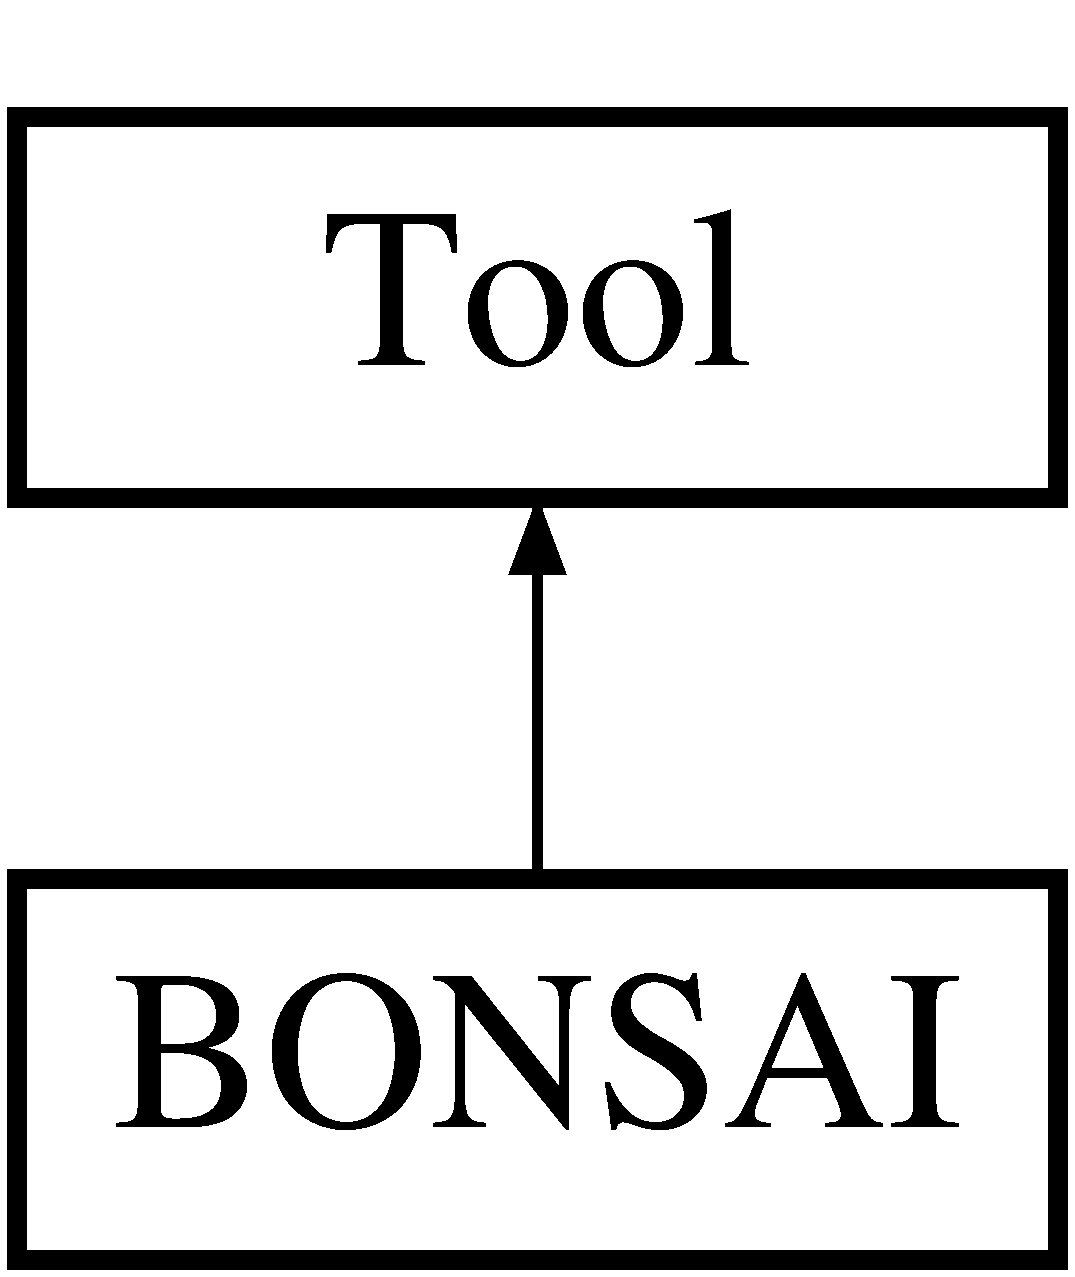
\includegraphics[height=2.000000cm]{classBONSAI}
\end{center}
\end{figure}
\subsection*{Public Member Functions}
\begin{DoxyCompactItemize}
\item 
\hypertarget{classBONSAI_a6f4e955fe871d3f87c9a086f8b27c23b}{bool {\bfseries Initialise} (std\-::string configfile, \hyperlink{classDataModel}{Data\-Model} \&data)}\label{classBONSAI_a6f4e955fe871d3f87c9a086f8b27c23b}

\item 
\hypertarget{classBONSAI_af232a6e7bbe7998f330a1b199e19d563}{bool {\bfseries Execute} ()}\label{classBONSAI_af232a6e7bbe7998f330a1b199e19d563}

\item 
\hypertarget{classBONSAI_aca309e129f0863903b826e3a9224ae72}{bool {\bfseries Finalise} ()}\label{classBONSAI_aca309e129f0863903b826e3a9224ae72}

\end{DoxyCompactItemize}


The documentation for this class was generated from the following files\-:\begin{DoxyCompactItemize}
\item 
User\-Tools/\-B\-O\-N\-S\-A\-I/B\-O\-N\-S\-A\-I.\-h\item 
User\-Tools/\-B\-O\-N\-S\-A\-I/B\-O\-N\-S\-A\-I.\-cpp\end{DoxyCompactItemize}

\hypertarget{structCherenkovCone}{\section{Cherenkov\-Cone Struct Reference}
\label{structCherenkovCone}\index{Cherenkov\-Cone@{Cherenkov\-Cone}}
}
\subsection*{Public Attributes}
\begin{DoxyCompactItemize}
\item 
\hypertarget{structCherenkovCone_a5dbbcf66d38890fbc33043bbd7f6bb12}{double {\bfseries cos\-\_\-angle}}\label{structCherenkovCone_a5dbbcf66d38890fbc33043bbd7f6bb12}

\item 
\hypertarget{structCherenkovCone_a81685c694d009b2d09a063986a2db932}{double {\bfseries ellipticity}}\label{structCherenkovCone_a81685c694d009b2d09a063986a2db932}

\end{DoxyCompactItemize}


The documentation for this struct was generated from the following file\-:\begin{DoxyCompactItemize}
\item 
Data\-Model/Recon\-Info.\-h\end{DoxyCompactItemize}

\hypertarget{classDataModel}{\section{Data\-Model Class Reference}
\label{classDataModel}\index{Data\-Model@{Data\-Model}}
}


{\ttfamily \#include $<$Data\-Model.\-h$>$}

\subsection*{Public Member Functions}
\begin{DoxyCompactItemize}
\item 
\hypertarget{classDataModel_abff03aef2cb531142a35781bb87c3365}{\hyperlink{classDataModel_abff03aef2cb531142a35781bb87c3365}{Data\-Model} ()}\label{classDataModel_abff03aef2cb531142a35781bb87c3365}

\begin{DoxyCompactList}\small\item\em Simple constructor. \end{DoxyCompactList}\item 
\hyperlink{classReconInfo}{Recon\-Info} $\ast$ \hyperlink{classDataModel_a1887c7e14241754c9967876de5b3495a}{Get\-Filter} (std\-::string name, bool can\-\_\-create)
\end{DoxyCompactItemize}
\subsection*{Public Attributes}
\begin{DoxyCompactItemize}
\item 
\hypertarget{classDataModel_a4baac5fe364a7a23762d70d2c2216486}{Store \hyperlink{classDataModel_a4baac5fe364a7a23762d70d2c2216486}{vars}}\label{classDataModel_a4baac5fe364a7a23762d70d2c2216486}

\begin{DoxyCompactList}\small\item\em This Store can be used for any variables. It is an inefficent ascii based storage. \end{DoxyCompactList}\item 
\hypertarget{classDataModel_a878e0d87285f0b3541a3e7116a5f00b6}{Boost\-Store \hyperlink{classDataModel_a878e0d87285f0b3541a3e7116a5f00b6}{C\-Store}}\label{classDataModel_a878e0d87285f0b3541a3e7116a5f00b6}

\begin{DoxyCompactList}\small\item\em This is a more efficent binary Boost\-Store that can be used to store a dynamic set of inter Tool variables. \end{DoxyCompactList}\item 
\hypertarget{classDataModel_ad1ffc080c3b263bf3ee382a531321ad4}{std\-::map$<$ std\-::string, \\*
Boost\-Store $\ast$ $>$ \hyperlink{classDataModel_ad1ffc080c3b263bf3ee382a531321ad4}{Stores}}\label{classDataModel_ad1ffc080c3b263bf3ee382a531321ad4}

\begin{DoxyCompactList}\small\item\em This is a map of named Boo\-Store pointers which can be deffined to hold a nammed collection of any tipe of Boost\-Store. It is usefull to store data that needs subdividing into differnt stores. \end{DoxyCompactList}\item 
\hypertarget{classDataModel_aa777da4c632e4659ee5b1447ad513458}{Logging $\ast$ \hyperlink{classDataModel_aa777da4c632e4659ee5b1447ad513458}{Log}}\label{classDataModel_aa777da4c632e4659ee5b1447ad513458}

\begin{DoxyCompactList}\small\item\em Log class pointer for use in Tools, it can be used to send messages which can have multiple error levels and destination end points. \end{DoxyCompactList}\item 
\hypertarget{classDataModel_a2c6dfd692e50f90e55338970ea7f8d61}{zmq\-::context\-\_\-t $\ast$ \hyperlink{classDataModel_a2c6dfd692e50f90e55338970ea7f8d61}{context}}\label{classDataModel_a2c6dfd692e50f90e55338970ea7f8d61}

\begin{DoxyCompactList}\small\item\em Z\-M\-Q contex used for producing zmq sockets for inter thread, process, or computer communication. \end{DoxyCompactList}\item 
\hypertarget{classDataModel_a117f5512507948489a7e726391c04324}{std\-::vector$<$ \hyperlink{classSubSample}{Sub\-Sample} $>$ \hyperlink{classDataModel_a117f5512507948489a7e726391c04324}{I\-D\-Samples}}\label{classDataModel_a117f5512507948489a7e726391c04324}

\begin{DoxyCompactList}\small\item\em Inner detector digit collections. \end{DoxyCompactList}\item 
\hypertarget{classDataModel_ac5669b4fb4e31fcb9525981ace801017}{std\-::vector$<$ \hyperlink{classSubSample}{Sub\-Sample} $>$ \hyperlink{classDataModel_ac5669b4fb4e31fcb9525981ace801017}{O\-D\-Samples}}\label{classDataModel_ac5669b4fb4e31fcb9525981ace801017}

\begin{DoxyCompactList}\small\item\em Outer detector digit collections. \end{DoxyCompactList}\item 
\hypertarget{classDataModel_a8b6ab332fa38b2ebfb686cb47e37a027}{std\-::vector$<$ \hyperlink{classPMTInfo}{P\-M\-T\-Info} $>$ \hyperlink{classDataModel_a8b6ab332fa38b2ebfb686cb47e37a027}{I\-D\-Geom}}\label{classDataModel_a8b6ab332fa38b2ebfb686cb47e37a027}

\begin{DoxyCompactList}\small\item\em Geometry information for the inner detector. \end{DoxyCompactList}\item 
\hypertarget{classDataModel_a71675824a1aef386894d876545f52094}{std\-::vector$<$ \hyperlink{classPMTInfo}{P\-M\-T\-Info} $>$ \hyperlink{classDataModel_a71675824a1aef386894d876545f52094}{O\-D\-Geom}}\label{classDataModel_a71675824a1aef386894d876545f52094}

\begin{DoxyCompactList}\small\item\em Geometry information for the outer detector. \end{DoxyCompactList}\item 
\hypertarget{classDataModel_a1ec2850822f07de49f6ddb05a8537881}{\hyperlink{classTriggerInfo}{Trigger\-Info} \hyperlink{classDataModel_a1ec2850822f07de49f6ddb05a8537881}{I\-D\-Triggers}}\label{classDataModel_a1ec2850822f07de49f6ddb05a8537881}

\begin{DoxyCompactList}\small\item\em Triggered time windows for the inner detector. \end{DoxyCompactList}\item 
\hypertarget{classDataModel_aac80402a18f6fcde9ec271211152e3a0}{\hyperlink{classTriggerInfo}{Trigger\-Info} \hyperlink{classDataModel_aac80402a18f6fcde9ec271211152e3a0}{O\-D\-Triggers}}\label{classDataModel_aac80402a18f6fcde9ec271211152e3a0}

\begin{DoxyCompactList}\small\item\em Triggered time windows for the outer detector. \end{DoxyCompactList}\item 
\hypertarget{classDataModel_a5471c8c372e061f47601f7c910e5d5c1}{bool \hyperlink{classDataModel_a5471c8c372e061f47601f7c910e5d5c1}{triggeroutput}}\label{classDataModel_a5471c8c372e061f47601f7c910e5d5c1}

\begin{DoxyCompactList}\small\item\em D\-E\-P\-R\-E\-C\-A\-T\-E\-D! Use I\-D\-Triggers and O\-D\-Triggers instead. \end{DoxyCompactList}\item 
\hypertarget{classDataModel_a3fa7b34f677cf748f48ac8e1ab43eddd}{\hyperlink{classReconInfo}{Recon\-Info} \hyperlink{classDataModel_a3fa7b34f677cf748f48ac8e1ab43eddd}{Reco\-Info}}\label{classDataModel_a3fa7b34f677cf748f48ac8e1ab43eddd}

\begin{DoxyCompactList}\small\item\em Store reconstruction information (vertex time/position, fit likelihoods, optionally direction) \end{DoxyCompactList}\item 
\hypertarget{classDataModel_a251e064bd60670ee4ac0eb94e42706ba}{std\-::map$<$ std\-::string, \\*
\hyperlink{classReconInfo}{Recon\-Info} $\ast$ $>$ \hyperlink{classDataModel_a251e064bd60670ee4ac0eb94e42706ba}{Reco\-Info\-Map}}\label{classDataModel_a251e064bd60670ee4ac0eb94e42706ba}

\begin{DoxyCompactList}\small\item\em Store filtered reconstruction information. \end{DoxyCompactList}\item 
\hypertarget{classDataModel_a402d65b5d38d1df743b148ff2050f30f}{double \hyperlink{classDataModel_a402d65b5d38d1df743b148ff2050f30f}{I\-D\-P\-M\-T\-Dark\-Rate}}\label{classDataModel_a402d65b5d38d1df743b148ff2050f30f}

\begin{DoxyCompactList}\small\item\em Dark noise rate of inner detector P\-M\-Ts, unit\-: ? \end{DoxyCompactList}\item 
\hypertarget{classDataModel_a30c2323b27be73a78886b527c8b43b30}{double \hyperlink{classDataModel_a30c2323b27be73a78886b527c8b43b30}{O\-D\-P\-M\-T\-Dark\-Rate}}\label{classDataModel_a30c2323b27be73a78886b527c8b43b30}

\begin{DoxyCompactList}\small\item\em Dark noise rate of outer detector P\-M\-Ts, unit\-: ? \end{DoxyCompactList}\item 
\hypertarget{classDataModel_a136ac1e3b7197b8d77ce09280ff38110}{int \hyperlink{classDataModel_a136ac1e3b7197b8d77ce09280ff38110}{I\-D\-N\-P\-M\-Ts}}\label{classDataModel_a136ac1e3b7197b8d77ce09280ff38110}

\begin{DoxyCompactList}\small\item\em Number of inner detector P\-M\-Ts. \end{DoxyCompactList}\item 
\hypertarget{classDataModel_a59c6f8afcab3b346d18d97b715763c1f}{int \hyperlink{classDataModel_a59c6f8afcab3b346d18d97b715763c1f}{O\-D\-N\-P\-M\-Ts}}\label{classDataModel_a59c6f8afcab3b346d18d97b715763c1f}

\begin{DoxyCompactList}\small\item\em Number of outer detector P\-M\-Ts. \end{DoxyCompactList}\item 
\hypertarget{classDataModel_ac64cb381d1cd620bcf8ecff268dc18e0}{double \hyperlink{classDataModel_ac64cb381d1cd620bcf8ecff268dc18e0}{detector\-\_\-length}}\label{classDataModel_ac64cb381d1cd620bcf8ecff268dc18e0}

\begin{DoxyCompactList}\small\item\em height of water tank \end{DoxyCompactList}\item 
\hypertarget{classDataModel_a2177924e78852c71c372749fffa1137d}{double \hyperlink{classDataModel_a2177924e78852c71c372749fffa1137d}{detector\-\_\-radius}}\label{classDataModel_a2177924e78852c71c372749fffa1137d}

\begin{DoxyCompactList}\small\item\em radius of water tank \end{DoxyCompactList}\item 
\hypertarget{classDataModel_a33c62502670e975cbc0e9ed6f0afa22f}{double \hyperlink{classDataModel_a33c62502670e975cbc0e9ed6f0afa22f}{pmt\-\_\-radius}}\label{classDataModel_a33c62502670e975cbc0e9ed6f0afa22f}

\begin{DoxyCompactList}\small\item\em radius of each P\-M\-T \end{DoxyCompactList}\item 
\hypertarget{classDataModel_aaff7bd723178271d795835e7d1e1dbef}{T\-Chain $\ast$ \hyperlink{classDataModel_aaff7bd723178271d795835e7d1e1dbef}{W\-C\-Sim\-Geom\-Tree}}\label{classDataModel_aaff7bd723178271d795835e7d1e1dbef}

\begin{DoxyCompactList}\small\item\em The {\ttfamily W\-C\-Sim\-Root\-Geom} tree from input W\-C\-Sim file(s) \end{DoxyCompactList}\item 
\hypertarget{classDataModel_a89cf7601bf57652b4a1363ec7dbc6dba}{T\-Chain $\ast$ \hyperlink{classDataModel_a89cf7601bf57652b4a1363ec7dbc6dba}{W\-C\-Sim\-Options\-Tree}}\label{classDataModel_a89cf7601bf57652b4a1363ec7dbc6dba}

\begin{DoxyCompactList}\small\item\em The {\ttfamily W\-C\-Sim\-Root\-Options} tree from input W\-C\-Sim file(s) \end{DoxyCompactList}\item 
\hypertarget{classDataModel_a5154cb6c2af332e5db8cf9c7620369f1}{T\-Chain $\ast$ \hyperlink{classDataModel_a5154cb6c2af332e5db8cf9c7620369f1}{W\-C\-Sim\-Event\-Tree}}\label{classDataModel_a5154cb6c2af332e5db8cf9c7620369f1}

\begin{DoxyCompactList}\small\item\em The {\ttfamily W\-C\-Sim\-Root\-Event} tree from input W\-C\-Sim file(s) \end{DoxyCompactList}\item 
\hypertarget{classDataModel_af13fe686acf2a60b84315c65f00af3cf}{int \hyperlink{classDataModel_af13fe686acf2a60b84315c65f00af3cf}{Current\-W\-C\-Sim\-Event\-Num}}\label{classDataModel_af13fe686acf2a60b84315c65f00af3cf}

\begin{DoxyCompactList}\small\item\em The original W\-C\-Sim files' event number for the current event. \end{DoxyCompactList}\item 
\hypertarget{classDataModel_ad368f473d985725a81a460595945c25b}{T\-Obj\-String \hyperlink{classDataModel_ad368f473d985725a81a460595945c25b}{Current\-W\-C\-Sim\-File}}\label{classDataModel_ad368f473d985725a81a460595945c25b}

\begin{DoxyCompactList}\small\item\em The original W\-C\-Sim files' filename for the current event. \end{DoxyCompactList}\item 
\hypertarget{classDataModel_a56a200514179bea6b890f71defbc604d}{W\-C\-Sim\-Root\-Event $\ast$ \hyperlink{classDataModel_a56a200514179bea6b890f71defbc604d}{I\-D\-W\-C\-Sim\-Event\-\_\-\-Raw}}\label{classDataModel_a56a200514179bea6b890f71defbc604d}

\begin{DoxyCompactList}\small\item\em The original, unmodified {\ttfamily W\-C\-Sim\-Root\-Event} for the I\-D. \end{DoxyCompactList}\item 
\hypertarget{classDataModel_a661853dc2ab04c2ef681cd0174fabe5c}{W\-C\-Sim\-Root\-Event $\ast$ \hyperlink{classDataModel_a661853dc2ab04c2ef681cd0174fabe5c}{O\-D\-W\-C\-Sim\-Event\-\_\-\-Raw}}\label{classDataModel_a661853dc2ab04c2ef681cd0174fabe5c}

\begin{DoxyCompactList}\small\item\em The original, unmodified {\ttfamily W\-C\-Sim\-Root\-Event} for the O\-D. \end{DoxyCompactList}\item 
\hypertarget{classDataModel_ab7b2e24128b6b1f3346c4e78009f75c7}{std\-::vector$<$ \hyperlink{structSNWarningParams}{S\-N\-Warning\-Params} $>$ \hyperlink{classDataModel_ab7b2e24128b6b1f3346c4e78009f75c7}{Supernova\-Warning\-Parameters}}\label{classDataModel_ab7b2e24128b6b1f3346c4e78009f75c7}

\begin{DoxyCompactList}\small\item\em Store the dimensionality, number of reconstructed vertices and the highest nclusters warning threshold passed. \end{DoxyCompactList}\item 
\hypertarget{classDataModel_a414da75f26f3460f26285bd815f1e1b3}{bool \hyperlink{classDataModel_a414da75f26f3460f26285bd815f1e1b3}{Has\-O\-D}}\label{classDataModel_a414da75f26f3460f26285bd815f1e1b3}

\begin{DoxyCompactList}\small\item\em Does the geometry include the outer detector? \end{DoxyCompactList}\item 
\hypertarget{classDataModel_a172f201ebabd4bd2ec50673a31d242df}{bool \hyperlink{classDataModel_a172f201ebabd4bd2ec50673a31d242df}{Is\-M\-C}}\label{classDataModel_a172f201ebabd4bd2ec50673a31d242df}

\begin{DoxyCompactList}\small\item\em Is this simulated data? \end{DoxyCompactList}\end{DoxyCompactItemize}


\subsection{Detailed Description}
This class Is a transient data model class for your Tools within the Tool\-Chain. If Tools need to comunicate they pass all data objects through the data model. There fore inter tool data objects should be deffined in this class.

\begin{DoxyParagraph}{Author\-:}
B.\-Richards 
\end{DoxyParagraph}
\begin{DoxyParagraph}{Date\-:}
2019/05/26 18\-:34\-:00 
\end{DoxyParagraph}
Contact\-: \href{mailto:b.richards@qmul.ac.uk}{\tt b.\-richards@qmul.\-ac.\-uk} 

\subsection{Member Function Documentation}
\hypertarget{classDataModel_a1887c7e14241754c9967876de5b3495a}{\index{Data\-Model@{Data\-Model}!Get\-Filter@{Get\-Filter}}
\index{Get\-Filter@{Get\-Filter}!DataModel@{Data\-Model}}
\subsubsection[{Get\-Filter}]{\setlength{\rightskip}{0pt plus 5cm}{\bf Recon\-Info} $\ast$ Data\-Model\-::\-Get\-Filter (
\begin{DoxyParamCaption}
\item[{std\-::string}]{name, }
\item[{bool}]{can\-\_\-create}
\end{DoxyParamCaption}
)}}\label{classDataModel_a1887c7e14241754c9967876de5b3495a}
Get filtered reconstructed information.

If {\ttfamily name == A\-L\-L}\-: pointer to all events ({\ttfamily Reco\-Info}) Otherwise, returns pointer to {\ttfamily Reco\-Info\-Map} entry name Caveat\-: if {\ttfamily !can\-\_\-create} and {\ttfamily name} not found, return {\ttfamily 0} 

The documentation for this class was generated from the following files\-:\begin{DoxyCompactItemize}
\item 
Data\-Model/Data\-Model.\-h\item 
Data\-Model/Data\-Model.\-cpp\end{DoxyCompactItemize}

\hypertarget{structDataModelThread__args}{\section{Data\-Model\-Thread\-\_\-args Struct Reference}
\label{structDataModelThread__args}\index{Data\-Model\-Thread\-\_\-args@{Data\-Model\-Thread\-\_\-args}}
}


{\ttfamily \#include $<$Utilities.\-h$>$}



\subsection{Detailed Description}
This is both an base class for any thread argument struct used in the tool threaded Tool templates. Effectivly this acts as a place to put variable that are specfic to that thread and can be used as a place to transfer variables from the main thread to sub threads.

\begin{DoxyParagraph}{Author\-:}
B.\-Richards 
\end{DoxyParagraph}
\begin{DoxyParagraph}{Date\-:}
2019/05/26 18\-:34\-:00 
\end{DoxyParagraph}
Contact\-: \href{mailto:b.richards@qmul.ac.uk}{\tt b.\-richards@qmul.\-ac.\-uk} 

The documentation for this struct was generated from the following file\-:\begin{DoxyCompactItemize}
\item 
Data\-Model/Utilities.\-h\end{DoxyCompactItemize}

\hypertarget{classDataOut}{\section{Data\-Out Class Reference}
\label{classDataOut}\index{Data\-Out@{Data\-Out}}
}
Inheritance diagram for Data\-Out\-:\begin{figure}[H]
\begin{center}
\leavevmode
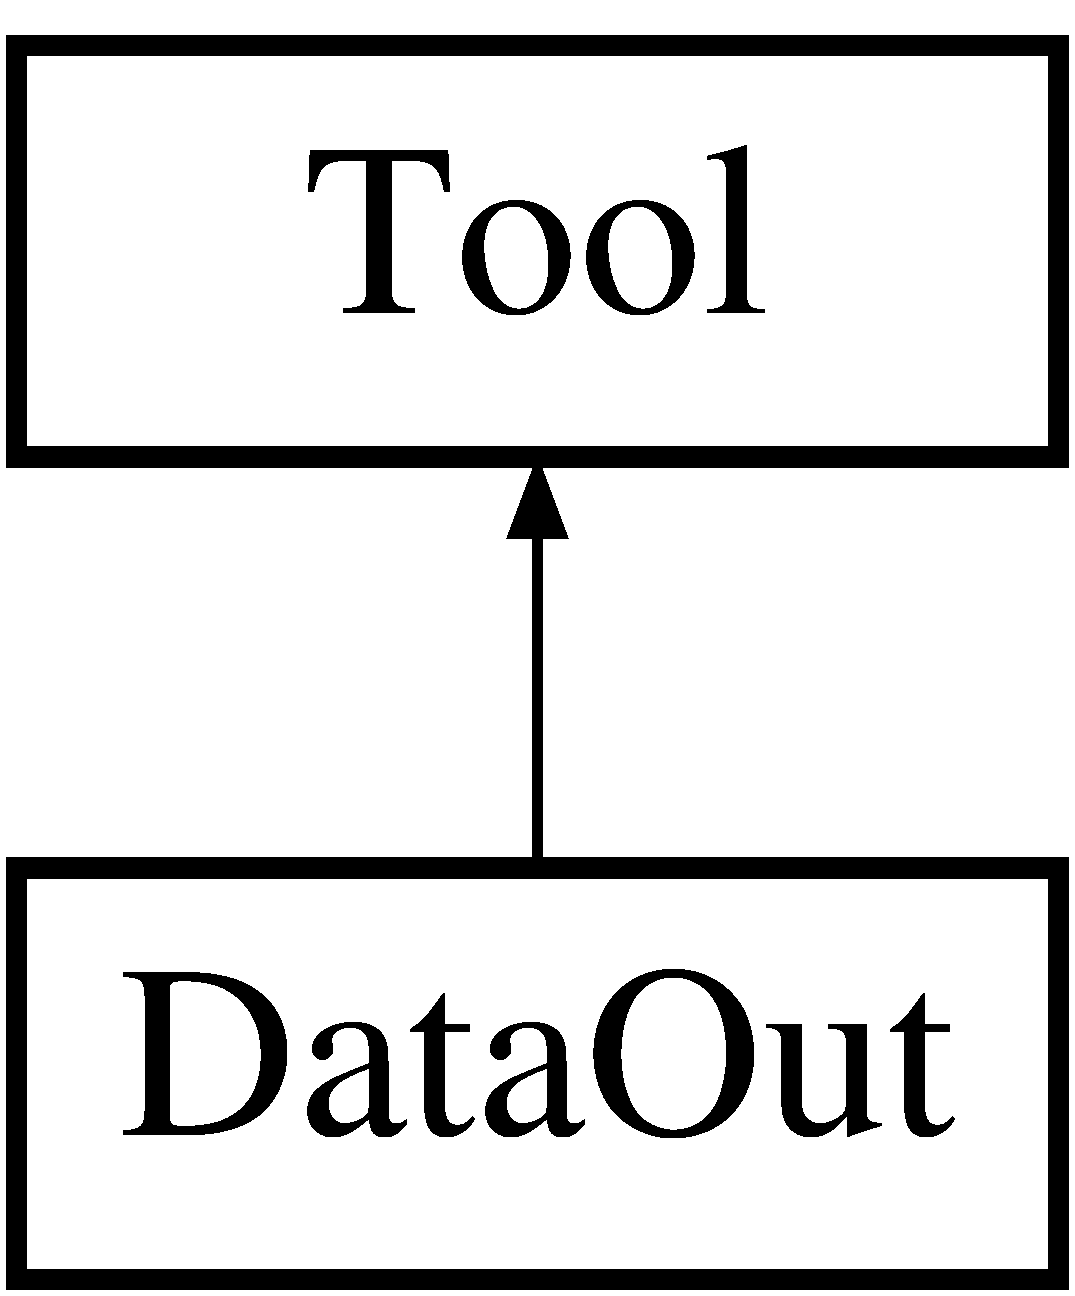
\includegraphics[height=2.000000cm]{classDataOut}
\end{center}
\end{figure}
\subsection*{Public Member Functions}
\begin{DoxyCompactItemize}
\item 
\hypertarget{classDataOut_ac79897fa3139ecccae928a1ae714841b}{bool {\bfseries Initialise} (std\-::string configfile, \hyperlink{classDataModel}{Data\-Model} \&data)}\label{classDataOut_ac79897fa3139ecccae928a1ae714841b}

\item 
\hypertarget{classDataOut_a9bcfadc03f76dde733dbf7a8aa1ed345}{bool {\bfseries Execute} ()}\label{classDataOut_a9bcfadc03f76dde733dbf7a8aa1ed345}

\item 
\hypertarget{classDataOut_a147ccd7146788b72a12f83f25fe3e487}{bool {\bfseries Finalise} ()}\label{classDataOut_a147ccd7146788b72a12f83f25fe3e487}

\end{DoxyCompactItemize}


The documentation for this class was generated from the following files\-:\begin{DoxyCompactItemize}
\item 
User\-Tools/\-Data\-Out/Data\-Out.\-h\item 
User\-Tools/\-Data\-Out/Data\-Out.\-cpp\end{DoxyCompactItemize}

\hypertarget{classdimfit}{\section{dimfit Class Reference}
\label{classdimfit}\index{dimfit@{dimfit}}
}
Inheritance diagram for dimfit\-:\begin{figure}[H]
\begin{center}
\leavevmode
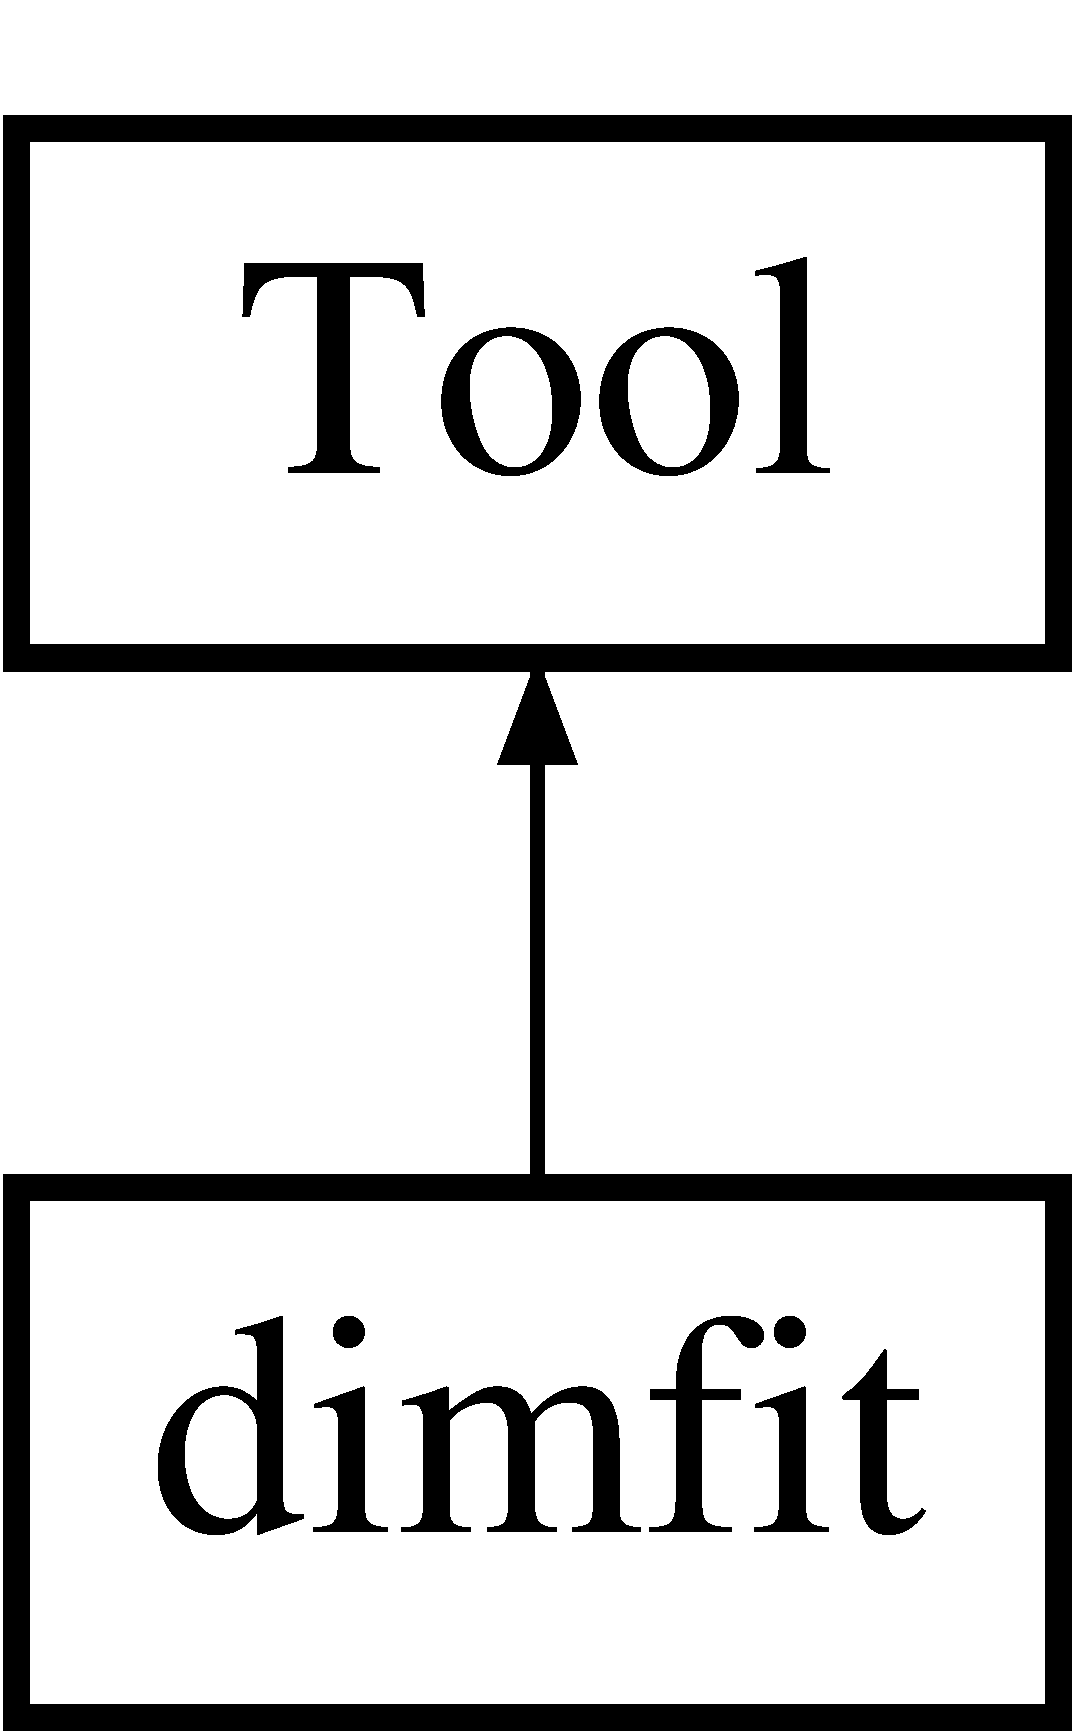
\includegraphics[height=2.000000cm]{classdimfit}
\end{center}
\end{figure}
\subsection*{Public Member Functions}
\begin{DoxyCompactItemize}
\item 
\hypertarget{classdimfit_a14db908c179f25acba98211d944dd3bd}{bool {\bfseries Initialise} (std\-::string configfile, \hyperlink{classDataModel}{Data\-Model} \&data)}\label{classdimfit_a14db908c179f25acba98211d944dd3bd}

\item 
\hypertarget{classdimfit_a214d0ff3e5268a3eccf7674d54f17bf6}{bool {\bfseries Execute} ()}\label{classdimfit_a214d0ff3e5268a3eccf7674d54f17bf6}

\item 
\hypertarget{classdimfit_a7f40e808c0af6512a53057748dc31c32}{bool {\bfseries Finalise} ()}\label{classdimfit_a7f40e808c0af6512a53057748dc31c32}

\end{DoxyCompactItemize}


The documentation for this class was generated from the following files\-:\begin{DoxyCompactItemize}
\item 
User\-Tools/dimfit/dimfit.\-h\item 
User\-Tools/dimfit/dimfit.\-cpp\end{DoxyCompactItemize}

\hypertarget{structDirectionEuler}{\section{Direction\-Euler Struct Reference}
\label{structDirectionEuler}\index{Direction\-Euler@{Direction\-Euler}}
}
\subsection*{Public Attributes}
\begin{DoxyCompactItemize}
\item 
\hypertarget{structDirectionEuler_afb5740bb67a68cf8845de3718ae058aa}{double {\bfseries theta}}\label{structDirectionEuler_afb5740bb67a68cf8845de3718ae058aa}

\item 
\hypertarget{structDirectionEuler_a8dc1a0f63653769875644cdbf7ecd36c}{double {\bfseries phi}}\label{structDirectionEuler_a8dc1a0f63653769875644cdbf7ecd36c}

\item 
\hypertarget{structDirectionEuler_a07ef38372e6bf743cef6e10f3a622910}{double {\bfseries alpha}}\label{structDirectionEuler_a07ef38372e6bf743cef6e10f3a622910}

\end{DoxyCompactItemize}


The documentation for this struct was generated from the following file\-:\begin{DoxyCompactItemize}
\item 
Data\-Model/Recon\-Info.\-h\end{DoxyCompactItemize}

\hypertarget{classDummyTool}{\section{Dummy\-Tool Class Reference}
\label{classDummyTool}\index{Dummy\-Tool@{Dummy\-Tool}}
}


{\ttfamily \#include $<$Dummy\-Tool.\-h$>$}

Inheritance diagram for Dummy\-Tool\-:\begin{figure}[H]
\begin{center}
\leavevmode
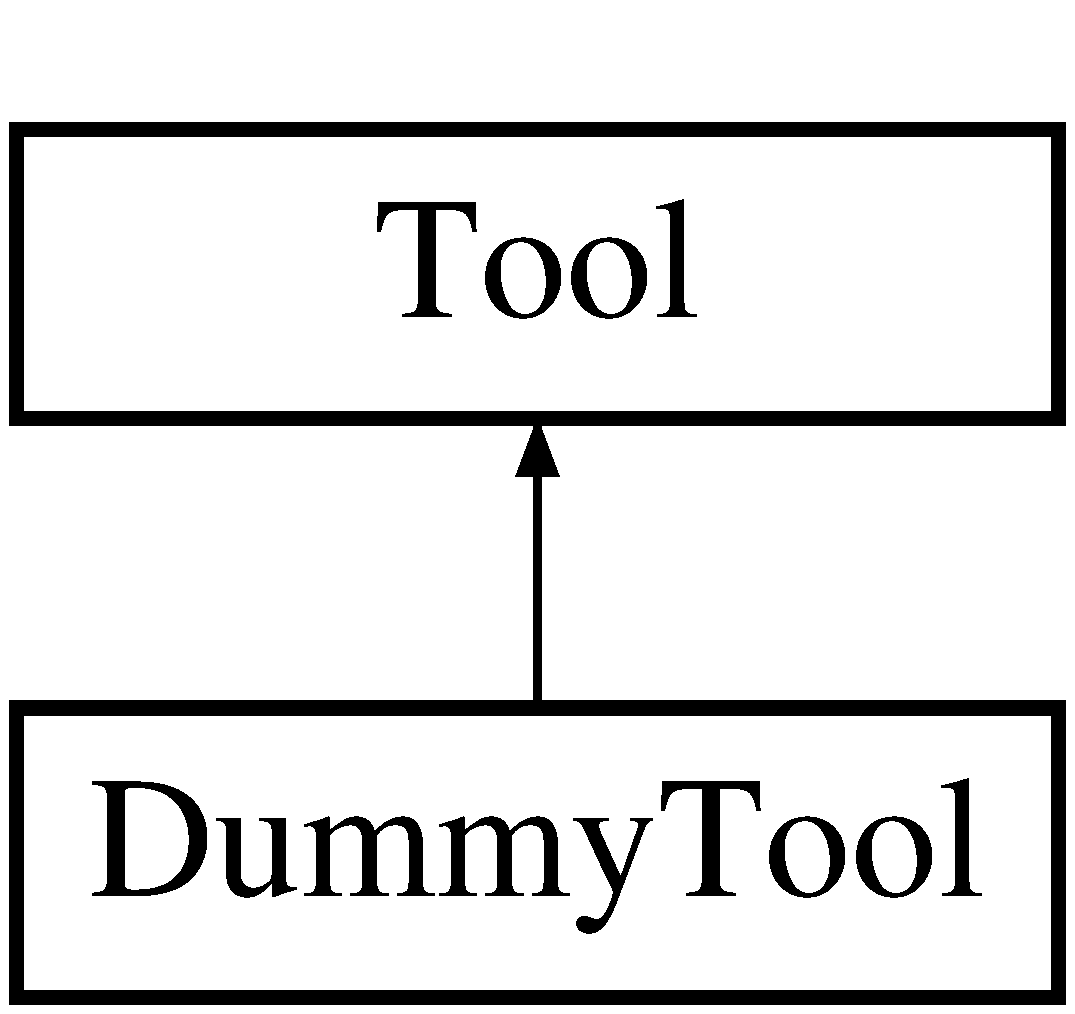
\includegraphics[height=2.000000cm]{classDummyTool}
\end{center}
\end{figure}
\subsection*{Public Member Functions}
\begin{DoxyCompactItemize}
\item 
\hypertarget{classDummyTool_a33914471b4de346168aa92b5febb6f9c}{\hyperlink{classDummyTool_a33914471b4de346168aa92b5febb6f9c}{Dummy\-Tool} ()}\label{classDummyTool_a33914471b4de346168aa92b5febb6f9c}

\begin{DoxyCompactList}\small\item\em Constructor. \end{DoxyCompactList}\item 
\hypertarget{classDummyTool_a0d9cd781681a06ee3cf0cd1e7bb770a8}{bool \hyperlink{classDummyTool_a0d9cd781681a06ee3cf0cd1e7bb770a8}{Initialise} (std\-::string configfile, \hyperlink{classDataModel}{Data\-Model} \&data)}\label{classDummyTool_a0d9cd781681a06ee3cf0cd1e7bb770a8}

\begin{DoxyCompactList}\small\item\em Assigns verbosity from config file and creates a log message. \end{DoxyCompactList}\item 
\hypertarget{classDummyTool_ac107b31f1785c1cc803e0e65be548047}{bool \hyperlink{classDummyTool_ac107b31f1785c1cc803e0e65be548047}{Execute} ()}\label{classDummyTool_ac107b31f1785c1cc803e0e65be548047}

\begin{DoxyCompactList}\small\item\em Creates a log message. \end{DoxyCompactList}\item 
\hypertarget{classDummyTool_aacb5d0b9906a27c2b4bba4aae9bc093a}{bool \hyperlink{classDummyTool_aacb5d0b9906a27c2b4bba4aae9bc093a}{Finalise} ()}\label{classDummyTool_aacb5d0b9906a27c2b4bba4aae9bc093a}

\begin{DoxyCompactList}\small\item\em Does nothing. \end{DoxyCompactList}\end{DoxyCompactItemize}


\subsection{Detailed Description}
This is a simple dummy Tool designed to show operation of a Tool. It also provides a default Tool for the Default Tool\-Chain.

\begin{DoxyParagraph}{Author\-:}
B.\-Richards 
\end{DoxyParagraph}
\begin{DoxyParagraph}{Date\-:}
2019/05/28 10\-:44\-:00 
\end{DoxyParagraph}
Contact\-: \href{mailto:b.richards@qmul.ac.uk}{\tt b.\-richards@qmul.\-ac.\-uk} 

The documentation for this class was generated from the following files\-:\begin{DoxyCompactItemize}
\item 
User\-Tools/\-Dummy\-Tool/Dummy\-Tool.\-h\item 
User\-Tools/\-Dummy\-Tool/Dummy\-Tool.\-cpp\end{DoxyCompactItemize}

\hypertarget{classFLOWERRecon}{\section{F\-L\-O\-W\-E\-R\-Recon Class Reference}
\label{classFLOWERRecon}\index{F\-L\-O\-W\-E\-R\-Recon@{F\-L\-O\-W\-E\-R\-Recon}}
}
Inheritance diagram for F\-L\-O\-W\-E\-R\-Recon\-:\begin{figure}[H]
\begin{center}
\leavevmode
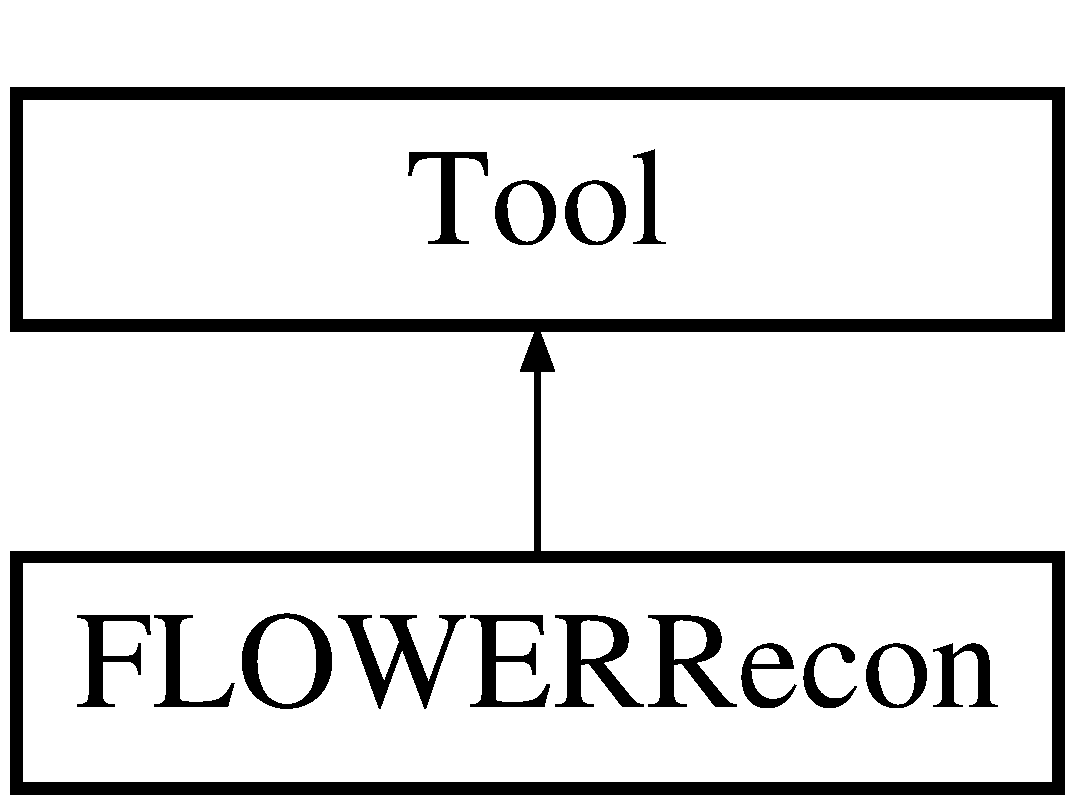
\includegraphics[height=2.000000cm]{classFLOWERRecon}
\end{center}
\end{figure}
\subsection*{Public Member Functions}
\begin{DoxyCompactItemize}
\item 
\hypertarget{classFLOWERRecon_a22d738c5f0d82306add530ae62613037}{bool {\bfseries Initialise} (std\-::string configfile, \hyperlink{classDataModel}{Data\-Model} \&data)}\label{classFLOWERRecon_a22d738c5f0d82306add530ae62613037}

\item 
\hypertarget{classFLOWERRecon_aafaf4c8c221737d6d5b984cee909f4e4}{bool {\bfseries Execute} ()}\label{classFLOWERRecon_aafaf4c8c221737d6d5b984cee909f4e4}

\item 
\hypertarget{classFLOWERRecon_a9e1c79216a6c4a9ab0025a3f5f55bb83}{bool {\bfseries Finalise} ()}\label{classFLOWERRecon_a9e1c79216a6c4a9ab0025a3f5f55bb83}

\end{DoxyCompactItemize}


The documentation for this class was generated from the following files\-:\begin{DoxyCompactItemize}
\item 
User\-Tools/\-F\-L\-O\-W\-E\-R\-Recon/F\-L\-O\-W\-E\-R\-Recon.\-h\item 
User\-Tools/\-F\-L\-O\-W\-E\-R\-Recon/F\-L\-O\-W\-E\-R\-Recon.\-cpp\end{DoxyCompactItemize}

\hypertarget{classMyTool}{\section{My\-Tool Class Reference}
\label{classMyTool}\index{My\-Tool@{My\-Tool}}
}


{\ttfamily \#include $<$My\-Tool.\-h$>$}

Inheritance diagram for My\-Tool\-:\begin{figure}[H]
\begin{center}
\leavevmode
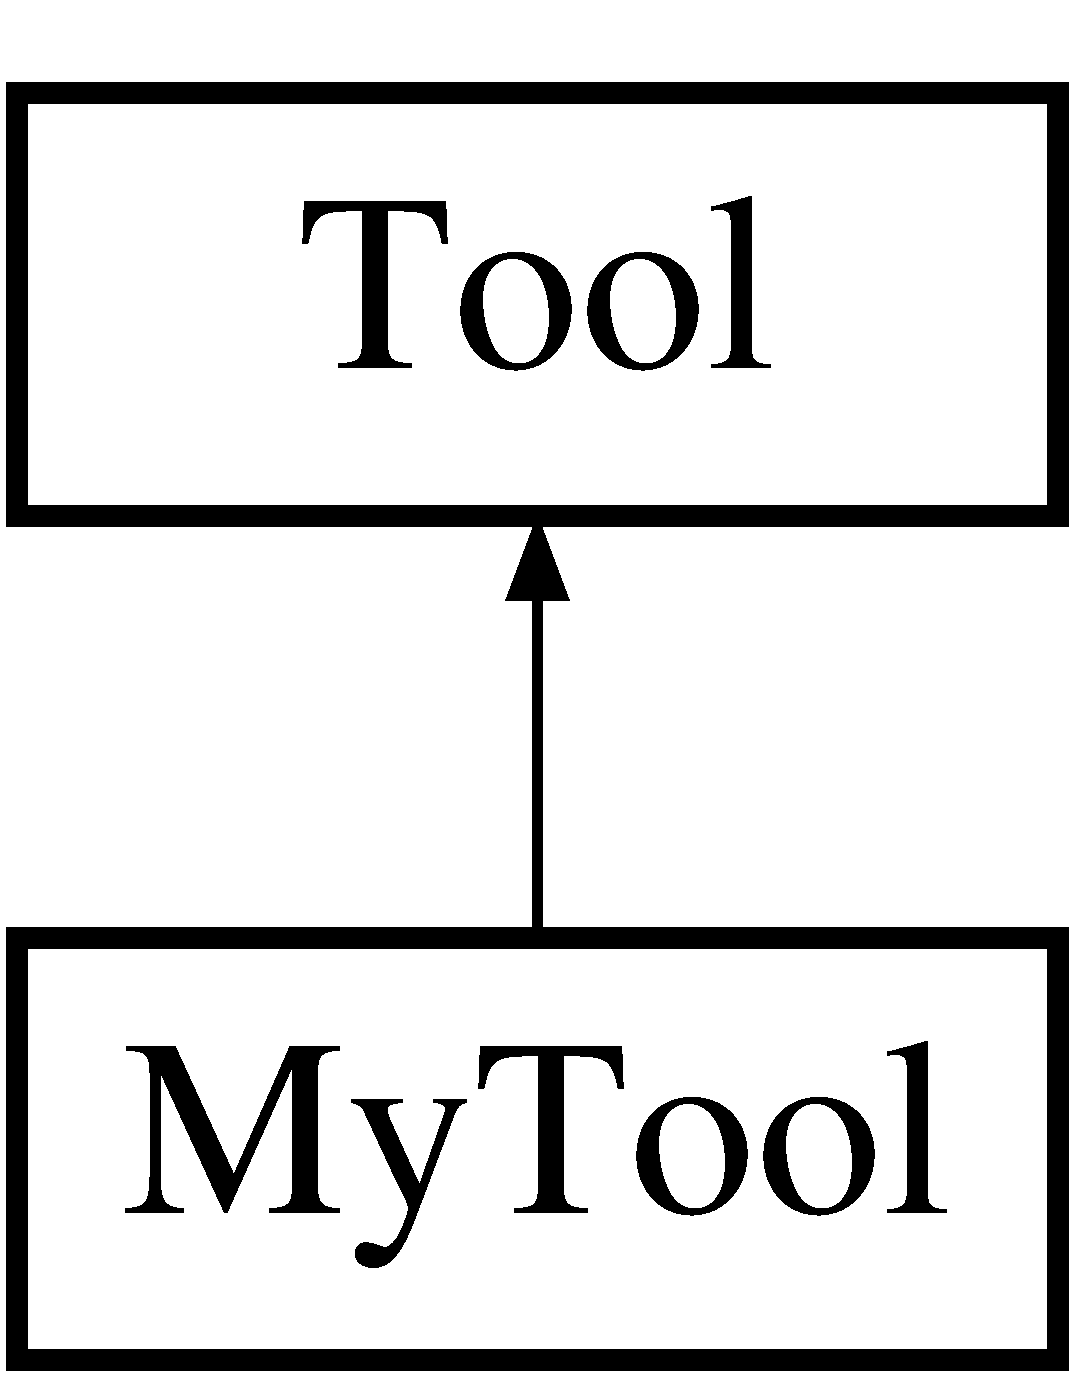
\includegraphics[height=2.000000cm]{classMyTool}
\end{center}
\end{figure}
\subsection*{Public Member Functions}
\begin{DoxyCompactItemize}
\item 
\hypertarget{classMyTool_ad85b796bdd675ae22e69cf40fe7b6314}{\hyperlink{classMyTool_ad85b796bdd675ae22e69cf40fe7b6314}{My\-Tool} ()}\label{classMyTool_ad85b796bdd675ae22e69cf40fe7b6314}

\begin{DoxyCompactList}\small\item\em Simple constructor. \end{DoxyCompactList}\item 
bool \hyperlink{classMyTool_a3bf60061195a18542c4cfb2916b9dad9}{Initialise} (std\-::string configfile, \hyperlink{classDataModel}{Data\-Model} \&data)
\begin{DoxyCompactList}\small\item\em Initialise Function for setting up Tool resorces. \end{DoxyCompactList}\item 
\hypertarget{classMyTool_a0a58122023af90b9200d0e71e89cfb36}{bool \hyperlink{classMyTool_a0a58122023af90b9200d0e71e89cfb36}{Execute} ()}\label{classMyTool_a0a58122023af90b9200d0e71e89cfb36}

\begin{DoxyCompactList}\small\item\em Executre function used to perform Tool perpose. \end{DoxyCompactList}\item 
\hypertarget{classMyTool_a060ec6356451aa335d0de41093c9992f}{bool \hyperlink{classMyTool_a060ec6356451aa335d0de41093c9992f}{Finalise} ()}\label{classMyTool_a060ec6356451aa335d0de41093c9992f}

\begin{DoxyCompactList}\small\item\em Finalise funciton used to clean up resorces. \end{DoxyCompactList}\end{DoxyCompactItemize}


\subsection{Detailed Description}
This is a balnk template for a Tool used by the script to generate a new custom tool. Please fill out the descripton and author information.

\begin{DoxyParagraph}{Author\-:}
B.\-Richards 
\end{DoxyParagraph}
\begin{DoxyParagraph}{Date\-:}
2019/05/28 10\-:44\-:00 
\end{DoxyParagraph}
Contact\-: \href{mailto:b.richards@qmul.ac.uk}{\tt b.\-richards@qmul.\-ac.\-uk} 

\subsection{Member Function Documentation}
\hypertarget{classMyTool_a3bf60061195a18542c4cfb2916b9dad9}{\index{My\-Tool@{My\-Tool}!Initialise@{Initialise}}
\index{Initialise@{Initialise}!MyTool@{My\-Tool}}
\subsubsection[{Initialise}]{\setlength{\rightskip}{0pt plus 5cm}bool My\-Tool\-::\-Initialise (
\begin{DoxyParamCaption}
\item[{std\-::string}]{configfile, }
\item[{{\bf Data\-Model} \&}]{data}
\end{DoxyParamCaption}
)}}\label{classMyTool_a3bf60061195a18542c4cfb2916b9dad9}


Initialise Function for setting up Tool resorces. 


\begin{DoxyParams}{Parameters}
{\em configfile} & The path and name of the dynamic configuration file to read in. \\
\hline
{\em data} & A reference to the transient data class used to pass information between Tools. \\
\hline
\end{DoxyParams}
Y\-O\-U\-R C\-O\-D\-E H\-E\-R\-E 

The documentation for this class was generated from the following files\-:\begin{DoxyCompactItemize}
\item 
User\-Tools/template/My\-Tool.\-h\item 
User\-Tools/template/My\-Tool.\-cpp\end{DoxyCompactItemize}

\hypertarget{classMyToolDynamicMultiThread}{\section{My\-Tool\-Dynamic\-Multi\-Thread Class Reference}
\label{classMyToolDynamicMultiThread}\index{My\-Tool\-Dynamic\-Multi\-Thread@{My\-Tool\-Dynamic\-Multi\-Thread}}
}


{\ttfamily \#include $<$My\-Tool\-Dynamic\-Multi\-Thread.\-h$>$}

Inheritance diagram for My\-Tool\-Dynamic\-Multi\-Thread\-:\begin{figure}[H]
\begin{center}
\leavevmode
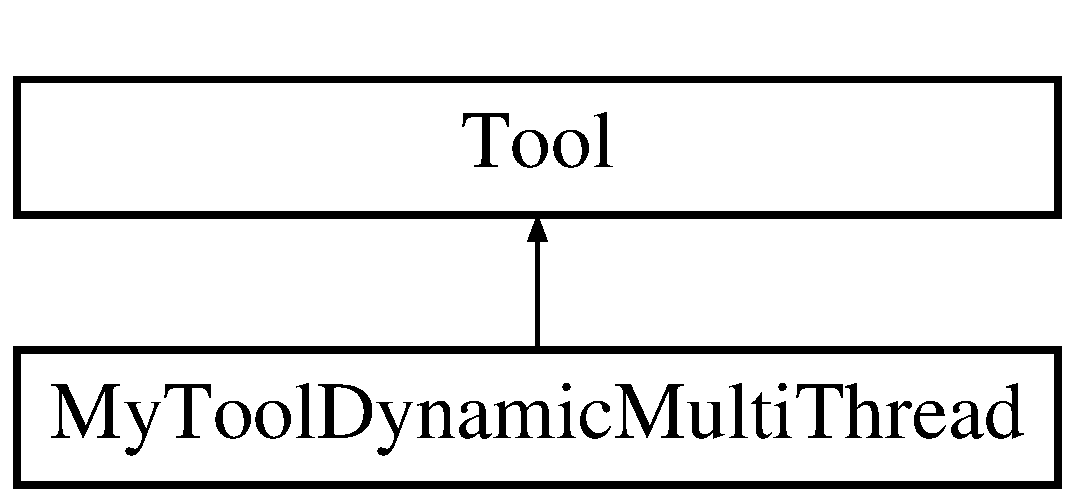
\includegraphics[height=2.000000cm]{classMyToolDynamicMultiThread}
\end{center}
\end{figure}
\subsection*{Public Member Functions}
\begin{DoxyCompactItemize}
\item 
\hypertarget{classMyToolDynamicMultiThread_a5eec7239400c507754ba6218b3eb8d4a}{\hyperlink{classMyToolDynamicMultiThread_a5eec7239400c507754ba6218b3eb8d4a}{My\-Tool\-Dynamic\-Multi\-Thread} ()}\label{classMyToolDynamicMultiThread_a5eec7239400c507754ba6218b3eb8d4a}

\begin{DoxyCompactList}\small\item\em Simple constructor. \end{DoxyCompactList}\item 
bool \hyperlink{classMyToolDynamicMultiThread_ac082408d85bc3e76214e55d4f62de0da}{Initialise} (std\-::string configfile, \hyperlink{classDataModel}{Data\-Model} \&data)
\begin{DoxyCompactList}\small\item\em Initialise Function for setting up Tool resorces. \end{DoxyCompactList}\item 
\hypertarget{classMyToolDynamicMultiThread_aec2f9af9495520d74bb154d626a94a63}{bool \hyperlink{classMyToolDynamicMultiThread_aec2f9af9495520d74bb154d626a94a63}{Execute} ()}\label{classMyToolDynamicMultiThread_aec2f9af9495520d74bb154d626a94a63}

\begin{DoxyCompactList}\small\item\em Executre function used to perform Tool perpose. \end{DoxyCompactList}\item 
\hypertarget{classMyToolDynamicMultiThread_ab70e77b0fd90e50c5103ccfa0bfd6485}{bool \hyperlink{classMyToolDynamicMultiThread_ab70e77b0fd90e50c5103ccfa0bfd6485}{Finalise} ()}\label{classMyToolDynamicMultiThread_ab70e77b0fd90e50c5103ccfa0bfd6485}

\begin{DoxyCompactList}\small\item\em Finalise funciton used to clean up resorces. \end{DoxyCompactList}\end{DoxyCompactItemize}


\subsection{Detailed Description}
This is a template for a Tool that dynamically more or less threads, such that there is always 1 available thread.\-This can therefore be used to scale to your worklaod, however be carefull when using more than one of these tools and to apply upperlimits if necessary both locally within this tool and globally so that more threads than is practical are created causing massive inefficency. Please fill out the descripton and author information.

\begin{DoxyParagraph}{Author\-:}
B.\-Richards 
\end{DoxyParagraph}
\begin{DoxyParagraph}{Date\-:}
2019/05/28 10\-:44\-:00 
\end{DoxyParagraph}
Contact\-: \href{mailto:b.richards@qmul.ac.uk}{\tt b.\-richards@qmul.\-ac.\-uk} 

\subsection{Member Function Documentation}
\hypertarget{classMyToolDynamicMultiThread_ac082408d85bc3e76214e55d4f62de0da}{\index{My\-Tool\-Dynamic\-Multi\-Thread@{My\-Tool\-Dynamic\-Multi\-Thread}!Initialise@{Initialise}}
\index{Initialise@{Initialise}!MyToolDynamicMultiThread@{My\-Tool\-Dynamic\-Multi\-Thread}}
\subsubsection[{Initialise}]{\setlength{\rightskip}{0pt plus 5cm}bool My\-Tool\-Dynamic\-Multi\-Thread\-::\-Initialise (
\begin{DoxyParamCaption}
\item[{std\-::string}]{configfile, }
\item[{{\bf Data\-Model} \&}]{data}
\end{DoxyParamCaption}
)}}\label{classMyToolDynamicMultiThread_ac082408d85bc3e76214e55d4f62de0da}


Initialise Function for setting up Tool resorces. 


\begin{DoxyParams}{Parameters}
{\em configfile} & The path and name of the dynamic configuration file to read in. \\
\hline
{\em data} & A reference to the transient data class used to pass information between Tools. \\
\hline
\end{DoxyParams}


The documentation for this class was generated from the following files\-:\begin{DoxyCompactItemize}
\item 
User\-Tools/template/My\-Tool\-Dynamic\-Multi\-Thread.\-h\item 
User\-Tools/template/My\-Tool\-Dynamic\-Multi\-Thread.\-cpp\end{DoxyCompactItemize}

\hypertarget{structMyToolDynamicMultiThread__args}{\section{My\-Tool\-Dynamic\-Multi\-Thread\-\_\-args Struct Reference}
\label{structMyToolDynamicMultiThread__args}\index{My\-Tool\-Dynamic\-Multi\-Thread\-\_\-args@{My\-Tool\-Dynamic\-Multi\-Thread\-\_\-args}}
}


{\ttfamily \#include $<$My\-Tool\-Dynamic\-Multi\-Thread.\-h$>$}

Inheritance diagram for My\-Tool\-Dynamic\-Multi\-Thread\-\_\-args\-:\begin{figure}[H]
\begin{center}
\leavevmode
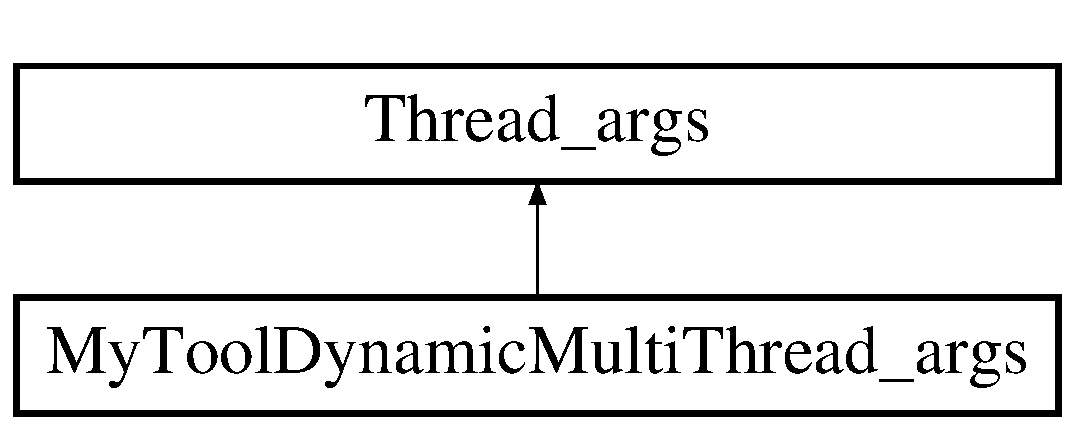
\includegraphics[height=2.000000cm]{structMyToolDynamicMultiThread__args}
\end{center}
\end{figure}
\subsection*{Public Attributes}
\begin{DoxyCompactItemize}
\item 
\hypertarget{structMyToolDynamicMultiThread__args_a2d4b96b18b6e91a4244473e9e28c881b}{bool {\bfseries busy}}\label{structMyToolDynamicMultiThread__args_a2d4b96b18b6e91a4244473e9e28c881b}

\item 
\hypertarget{structMyToolDynamicMultiThread__args_a4fe59813f550a1c10a2ab6527c580a23}{std\-::string {\bfseries message}}\label{structMyToolDynamicMultiThread__args_a4fe59813f550a1c10a2ab6527c580a23}

\end{DoxyCompactItemize}
\subsection*{Additional Inherited Members}


\subsection{Detailed Description}
This is a struct to place data you want your thread to acess or exchange with it. The idea is the datainside is only used by the threa\textbackslash{} d and so will be thread safe

\begin{DoxyParagraph}{Author\-:}
B.\-Richards 
\end{DoxyParagraph}
\begin{DoxyParagraph}{Date\-:}
2019/05/28 10\-:44\-:00 
\end{DoxyParagraph}
Contact\-: \href{mailto:b.richards@qmul.ac.uk}{\tt b.\-richards@qmul.\-ac.\-uk} 

The documentation for this struct was generated from the following files\-:\begin{DoxyCompactItemize}
\item 
User\-Tools/template/My\-Tool\-Dynamic\-Multi\-Thread.\-h\item 
User\-Tools/template/My\-Tool\-Dynamic\-Multi\-Thread.\-cpp\end{DoxyCompactItemize}

\hypertarget{classMyToolMultiThread}{\section{My\-Tool\-Multi\-Thread Class Reference}
\label{classMyToolMultiThread}\index{My\-Tool\-Multi\-Thread@{My\-Tool\-Multi\-Thread}}
}


{\ttfamily \#include $<$My\-Tool\-Multi\-Thread.\-h$>$}

Inheritance diagram for My\-Tool\-Multi\-Thread\-:\begin{figure}[H]
\begin{center}
\leavevmode
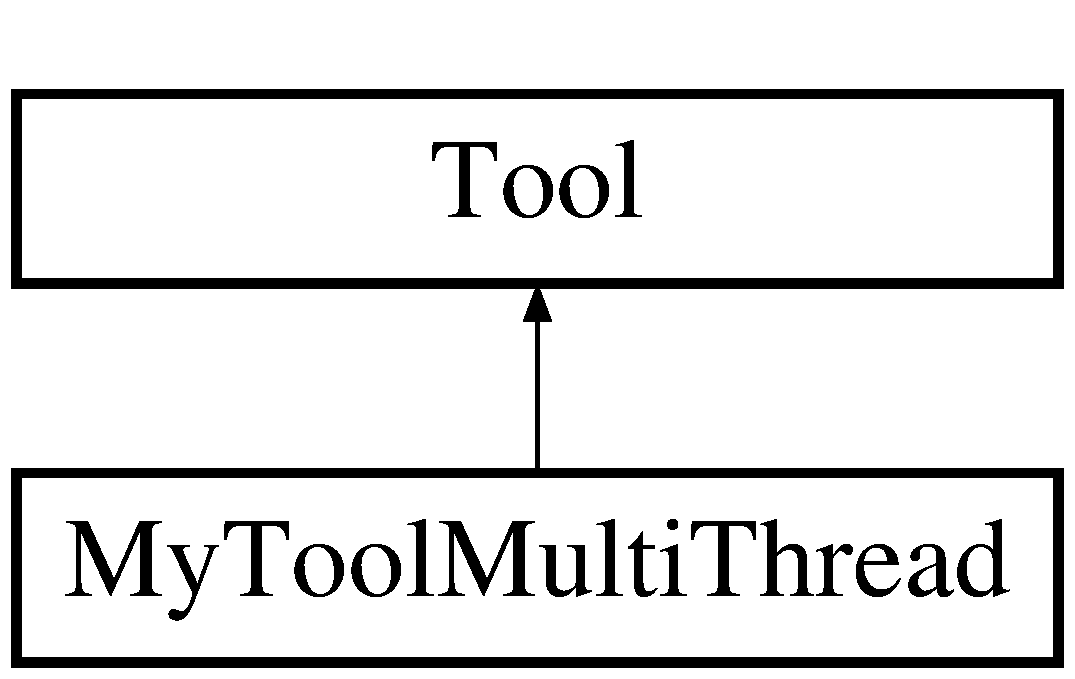
\includegraphics[height=2.000000cm]{classMyToolMultiThread}
\end{center}
\end{figure}
\subsection*{Public Member Functions}
\begin{DoxyCompactItemize}
\item 
\hypertarget{classMyToolMultiThread_ac24f005c6da9c552871f6ff2672cf7f1}{\hyperlink{classMyToolMultiThread_ac24f005c6da9c552871f6ff2672cf7f1}{My\-Tool\-Multi\-Thread} ()}\label{classMyToolMultiThread_ac24f005c6da9c552871f6ff2672cf7f1}

\begin{DoxyCompactList}\small\item\em Simple constructor. \end{DoxyCompactList}\item 
bool \hyperlink{classMyToolMultiThread_a19dc55079a7b2da02ad9addd565b8e80}{Initialise} (std\-::string configfile, \hyperlink{classDataModel}{Data\-Model} \&data)
\begin{DoxyCompactList}\small\item\em Initialise Function for setting up Tool resorces. \end{DoxyCompactList}\item 
\hypertarget{classMyToolMultiThread_a9cd7c894fc4797b2d81e12e25eb5beec}{bool \hyperlink{classMyToolMultiThread_a9cd7c894fc4797b2d81e12e25eb5beec}{Execute} ()}\label{classMyToolMultiThread_a9cd7c894fc4797b2d81e12e25eb5beec}

\begin{DoxyCompactList}\small\item\em Executre function used to perform Tool perpose. \end{DoxyCompactList}\item 
\hypertarget{classMyToolMultiThread_a8f25561dc6a5daf8f4db85afecbb2c38}{bool \hyperlink{classMyToolMultiThread_a8f25561dc6a5daf8f4db85afecbb2c38}{Finalise} ()}\label{classMyToolMultiThread_a8f25561dc6a5daf8f4db85afecbb2c38}

\begin{DoxyCompactList}\small\item\em Finalise funciton used to clean up resorces. \end{DoxyCompactList}\end{DoxyCompactItemize}


\subsection{Detailed Description}
This is a template for a Tool That employs mulitple threads. Please fill out the descripton and author information.

\begin{DoxyParagraph}{Author\-:}
B.\-Richards 
\end{DoxyParagraph}
\begin{DoxyParagraph}{Date\-:}
2019/05/28 10\-:44\-:00 
\end{DoxyParagraph}
Contact\-: \href{mailto:b.richards@qmul.ac.uk}{\tt b.\-richards@qmul.\-ac.\-uk} 

\subsection{Member Function Documentation}
\hypertarget{classMyToolMultiThread_a19dc55079a7b2da02ad9addd565b8e80}{\index{My\-Tool\-Multi\-Thread@{My\-Tool\-Multi\-Thread}!Initialise@{Initialise}}
\index{Initialise@{Initialise}!MyToolMultiThread@{My\-Tool\-Multi\-Thread}}
\subsubsection[{Initialise}]{\setlength{\rightskip}{0pt plus 5cm}bool My\-Tool\-Multi\-Thread\-::\-Initialise (
\begin{DoxyParamCaption}
\item[{std\-::string}]{configfile, }
\item[{{\bf Data\-Model} \&}]{data}
\end{DoxyParamCaption}
)}}\label{classMyToolMultiThread_a19dc55079a7b2da02ad9addd565b8e80}


Initialise Function for setting up Tool resorces. 


\begin{DoxyParams}{Parameters}
{\em configfile} & The path and name of the dynamic configuration file to read in. \\
\hline
{\em data} & A reference to the transient data class used to pass information between Tools. \\
\hline
\end{DoxyParams}


The documentation for this class was generated from the following files\-:\begin{DoxyCompactItemize}
\item 
User\-Tools/template/My\-Tool\-Multi\-Thread.\-h\item 
User\-Tools/template/My\-Tool\-Multi\-Thread.\-cpp\end{DoxyCompactItemize}

\hypertarget{structMyToolMultiThread__args}{\section{My\-Tool\-Multi\-Thread\-\_\-args Struct Reference}
\label{structMyToolMultiThread__args}\index{My\-Tool\-Multi\-Thread\-\_\-args@{My\-Tool\-Multi\-Thread\-\_\-args}}
}


{\ttfamily \#include $<$My\-Tool\-Multi\-Thread.\-h$>$}

Inheritance diagram for My\-Tool\-Multi\-Thread\-\_\-args\-:\begin{figure}[H]
\begin{center}
\leavevmode
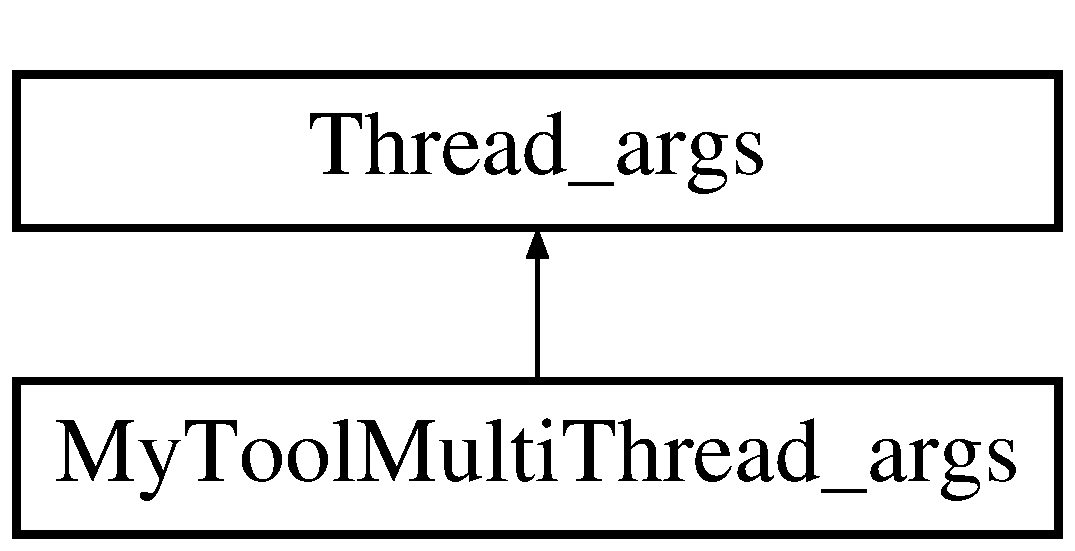
\includegraphics[height=2.000000cm]{structMyToolMultiThread__args}
\end{center}
\end{figure}
\subsection*{Public Attributes}
\begin{DoxyCompactItemize}
\item 
\hypertarget{structMyToolMultiThread__args_a25e00c4f60078d432869910f475fff9b}{bool {\bfseries busy}}\label{structMyToolMultiThread__args_a25e00c4f60078d432869910f475fff9b}

\item 
\hypertarget{structMyToolMultiThread__args_a05324a4ea6b7c87b2cc09473ab9027f5}{std\-::string {\bfseries message}}\label{structMyToolMultiThread__args_a05324a4ea6b7c87b2cc09473ab9027f5}

\end{DoxyCompactItemize}
\subsection*{Additional Inherited Members}


\subsection{Detailed Description}
This is a struct to place data you want your thread to acess or exchange with it. The idea is the datainside is only used by the thread and so will be thread safe

\begin{DoxyParagraph}{Author\-:}
B.\-Richards 
\end{DoxyParagraph}
\begin{DoxyParagraph}{Date\-:}
2019/05/28 10\-:44\-:00 
\end{DoxyParagraph}
Contact\-: \href{mailto:b.richards@qmul.ac.uk}{\tt b.\-richards@qmul.\-ac.\-uk} 

The documentation for this struct was generated from the following files\-:\begin{DoxyCompactItemize}
\item 
User\-Tools/template/My\-Tool\-Multi\-Thread.\-h\item 
User\-Tools/template/My\-Tool\-Multi\-Thread.\-cpp\end{DoxyCompactItemize}

\hypertarget{classMyToolServiceAdd}{\section{My\-Tool\-Service\-Add Class Reference}
\label{classMyToolServiceAdd}\index{My\-Tool\-Service\-Add@{My\-Tool\-Service\-Add}}
}


{\ttfamily \#include $<$My\-Tool\-Service\-Add.\-h$>$}

Inheritance diagram for My\-Tool\-Service\-Add\-:\begin{figure}[H]
\begin{center}
\leavevmode
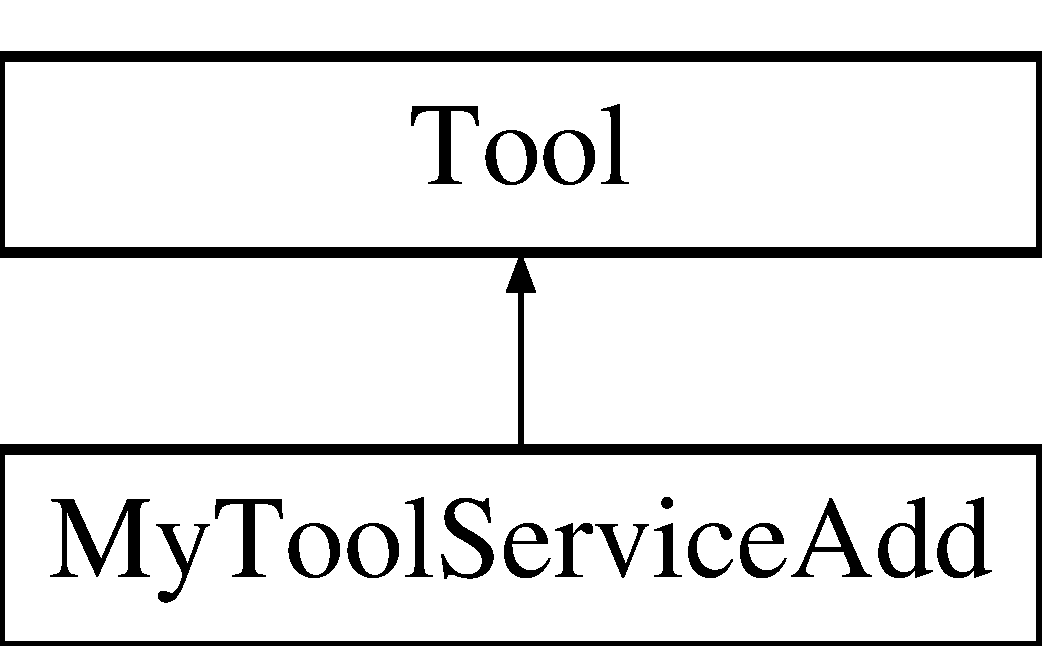
\includegraphics[height=2.000000cm]{classMyToolServiceAdd}
\end{center}
\end{figure}
\subsection*{Public Member Functions}
\begin{DoxyCompactItemize}
\item 
\hypertarget{classMyToolServiceAdd_a74ea27af61207cb9542f569e5669f013}{\hyperlink{classMyToolServiceAdd_a74ea27af61207cb9542f569e5669f013}{My\-Tool\-Service\-Add} ()}\label{classMyToolServiceAdd_a74ea27af61207cb9542f569e5669f013}

\begin{DoxyCompactList}\small\item\em Simple constructor. \end{DoxyCompactList}\item 
bool \hyperlink{classMyToolServiceAdd_a4b97306d13efe59a0a4cc8ca0f1560ea}{Initialise} (std\-::string configfile, \hyperlink{classDataModel}{Data\-Model} \&data)
\begin{DoxyCompactList}\small\item\em Initialise Function for setting up Tool resorces. \end{DoxyCompactList}\item 
\hypertarget{classMyToolServiceAdd_a876f8dac7b415b064d09687abac8e296}{bool \hyperlink{classMyToolServiceAdd_a876f8dac7b415b064d09687abac8e296}{Execute} ()}\label{classMyToolServiceAdd_a876f8dac7b415b064d09687abac8e296}

\begin{DoxyCompactList}\small\item\em Executre function used to perform Tool perpose. \end{DoxyCompactList}\item 
\hypertarget{classMyToolServiceAdd_a7ce3453fe2e9e626f6b47a10aa2d1050}{bool \hyperlink{classMyToolServiceAdd_a7ce3453fe2e9e626f6b47a10aa2d1050}{Finalise} ()}\label{classMyToolServiceAdd_a7ce3453fe2e9e626f6b47a10aa2d1050}

\begin{DoxyCompactList}\small\item\em Finalise funciton used to clean up resorces. \end{DoxyCompactList}\end{DoxyCompactItemize}


\subsection{Detailed Description}
This is a template for a Tool to publish a service via Tool\-D\-A\-Q dynamic service discovery. Please fill out the descripton and author information.

\begin{DoxyParagraph}{Author\-:}
B.\-Richards 
\end{DoxyParagraph}
\begin{DoxyParagraph}{Date\-:}
2019/05/28 10\-:44\-:00 
\end{DoxyParagraph}
Contact\-: \href{mailto:b.richards@qmul.ac.uk}{\tt b.\-richards@qmul.\-ac.\-uk} 

\subsection{Member Function Documentation}
\hypertarget{classMyToolServiceAdd_a4b97306d13efe59a0a4cc8ca0f1560ea}{\index{My\-Tool\-Service\-Add@{My\-Tool\-Service\-Add}!Initialise@{Initialise}}
\index{Initialise@{Initialise}!MyToolServiceAdd@{My\-Tool\-Service\-Add}}
\subsubsection[{Initialise}]{\setlength{\rightskip}{0pt plus 5cm}bool My\-Tool\-Service\-Add\-::\-Initialise (
\begin{DoxyParamCaption}
\item[{std\-::string}]{configfile, }
\item[{{\bf Data\-Model} \&}]{data}
\end{DoxyParamCaption}
)}}\label{classMyToolServiceAdd_a4b97306d13efe59a0a4cc8ca0f1560ea}


Initialise Function for setting up Tool resorces. 


\begin{DoxyParams}{Parameters}
{\em configfile} & The path and name of the dynamic configuration file to read in. \\
\hline
{\em data} & A reference to the transient data class used to pass information between Tools. \\
\hline
\end{DoxyParams}


The documentation for this class was generated from the following files\-:\begin{DoxyCompactItemize}
\item 
User\-Tools/template/My\-Tool\-Service\-Add.\-h\item 
User\-Tools/template/My\-Tool\-Service\-Add.\-cpp\end{DoxyCompactItemize}

\hypertarget{classMyToolThread}{\section{My\-Tool\-Thread Class Reference}
\label{classMyToolThread}\index{My\-Tool\-Thread@{My\-Tool\-Thread}}
}


{\ttfamily \#include $<$My\-Tool\-Thread.\-h$>$}

Inheritance diagram for My\-Tool\-Thread\-:\begin{figure}[H]
\begin{center}
\leavevmode
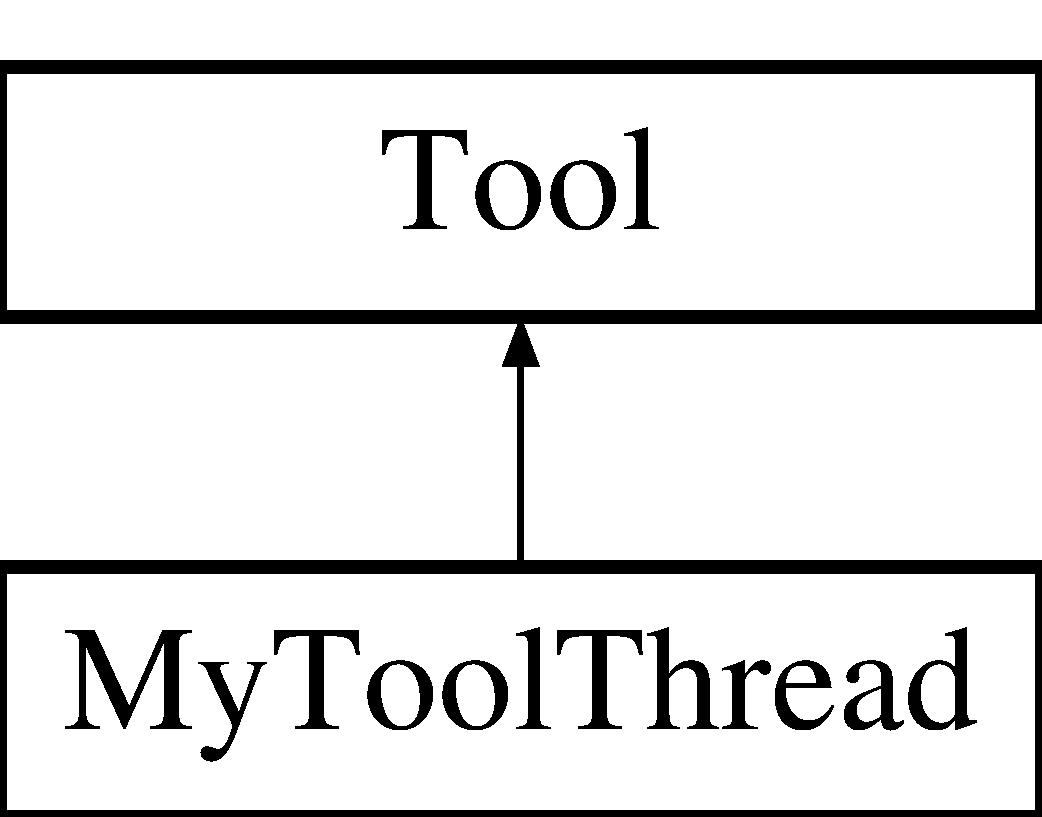
\includegraphics[height=2.000000cm]{classMyToolThread}
\end{center}
\end{figure}
\subsection*{Public Member Functions}
\begin{DoxyCompactItemize}
\item 
\hypertarget{classMyToolThread_a66c6fc304a8d62436281598d988dd845}{\hyperlink{classMyToolThread_a66c6fc304a8d62436281598d988dd845}{My\-Tool\-Thread} ()}\label{classMyToolThread_a66c6fc304a8d62436281598d988dd845}

\begin{DoxyCompactList}\small\item\em Simple constructor. \end{DoxyCompactList}\item 
bool \hyperlink{classMyToolThread_adc7ab1ab74fc1564f07e52e63383d679}{Initialise} (std\-::string configfile, \hyperlink{classDataModel}{Data\-Model} \&data)
\begin{DoxyCompactList}\small\item\em Initialise Function for setting up Tool resorces. \end{DoxyCompactList}\item 
\hypertarget{classMyToolThread_a9b582cd202d5578682d57d973988df3c}{bool \hyperlink{classMyToolThread_a9b582cd202d5578682d57d973988df3c}{Execute} ()}\label{classMyToolThread_a9b582cd202d5578682d57d973988df3c}

\begin{DoxyCompactList}\small\item\em Executre function used to perform Tool perpose. \end{DoxyCompactList}\item 
\hypertarget{classMyToolThread_aa51e385684efcb19f1c039b96653070e}{bool \hyperlink{classMyToolThread_aa51e385684efcb19f1c039b96653070e}{Finalise} ()}\label{classMyToolThread_aa51e385684efcb19f1c039b96653070e}

\begin{DoxyCompactList}\small\item\em Finalise funciton used to clean up resorces. \end{DoxyCompactList}\end{DoxyCompactItemize}


\subsection{Detailed Description}
This is a template for a Tool that produces a single thread that can be assigned a function seperate to the main thread. Please fill out the descripton and author information.

\begin{DoxyParagraph}{Author\-:}
B.\-Richards 
\end{DoxyParagraph}
\begin{DoxyParagraph}{Date\-:}
2019/05/28 10\-:44\-:00 
\end{DoxyParagraph}
Contact\-: \href{mailto:b.richards@qmul.ac.uk}{\tt b.\-richards@qmul.\-ac.\-uk} 

\subsection{Member Function Documentation}
\hypertarget{classMyToolThread_adc7ab1ab74fc1564f07e52e63383d679}{\index{My\-Tool\-Thread@{My\-Tool\-Thread}!Initialise@{Initialise}}
\index{Initialise@{Initialise}!MyToolThread@{My\-Tool\-Thread}}
\subsubsection[{Initialise}]{\setlength{\rightskip}{0pt plus 5cm}bool My\-Tool\-Thread\-::\-Initialise (
\begin{DoxyParamCaption}
\item[{std\-::string}]{configfile, }
\item[{{\bf Data\-Model} \&}]{data}
\end{DoxyParamCaption}
)}}\label{classMyToolThread_adc7ab1ab74fc1564f07e52e63383d679}


Initialise Function for setting up Tool resorces. 


\begin{DoxyParams}{Parameters}
{\em configfile} & The path and name of the dynamic configuration file to read in. \\
\hline
{\em data} & A reference to the transient data class used to pass information between Tools. \\
\hline
\end{DoxyParams}


The documentation for this class was generated from the following files\-:\begin{DoxyCompactItemize}
\item 
User\-Tools/template/My\-Tool\-Thread.\-h\item 
User\-Tools/template/My\-Tool\-Thread.\-cpp\end{DoxyCompactItemize}

\hypertarget{structMyToolThread__args}{\section{My\-Tool\-Thread\-\_\-args Struct Reference}
\label{structMyToolThread__args}\index{My\-Tool\-Thread\-\_\-args@{My\-Tool\-Thread\-\_\-args}}
}
Inheritance diagram for My\-Tool\-Thread\-\_\-args\-:\begin{figure}[H]
\begin{center}
\leavevmode
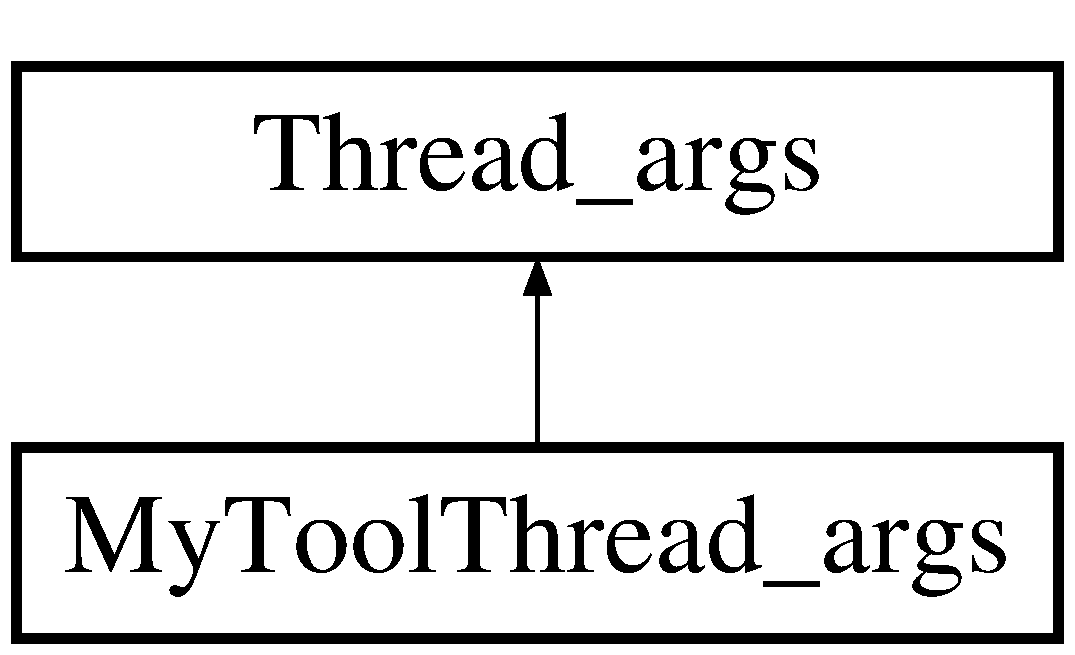
\includegraphics[height=2.000000cm]{structMyToolThread__args}
\end{center}
\end{figure}
\subsection*{Additional Inherited Members}


The documentation for this struct was generated from the following files\-:\begin{DoxyCompactItemize}
\item 
User\-Tools/template/My\-Tool\-Thread.\-h\item 
User\-Tools/template/My\-Tool\-Thread.\-cpp\end{DoxyCompactItemize}

\hypertarget{structMyToolThread__args__args}{\section{My\-Tool\-Thread\-\_\-args\-\_\-args Struct Reference}
\label{structMyToolThread__args__args}\index{My\-Tool\-Thread\-\_\-args\-\_\-args@{My\-Tool\-Thread\-\_\-args\-\_\-args}}
}


{\ttfamily \#include $<$My\-Tool\-Thread.\-h$>$}



\subsection{Detailed Description}
This is a struct to place data you want your thread to access or exchange with it. The idea is the datainside is only used by the threa and so will be thread safe

\begin{DoxyParagraph}{Author\-:}
B.\-Richards 
\end{DoxyParagraph}
\begin{DoxyParagraph}{Date\-:}
2019/05/28 10\-:44\-:00 
\end{DoxyParagraph}
Contact\-: \href{mailto:b.richards@qmul.ac.uk}{\tt b.\-richards@qmul.\-ac.\-uk} 

The documentation for this struct was generated from the following file\-:\begin{DoxyCompactItemize}
\item 
User\-Tools/template/My\-Tool\-Thread.\-h\end{DoxyCompactItemize}

\hypertarget{classMyToolZMQMultiThread}{\section{My\-Tool\-Z\-M\-Q\-Multi\-Thread Class Reference}
\label{classMyToolZMQMultiThread}\index{My\-Tool\-Z\-M\-Q\-Multi\-Thread@{My\-Tool\-Z\-M\-Q\-Multi\-Thread}}
}


{\ttfamily \#include $<$My\-Tool\-Z\-M\-Q\-Multi\-Thread.\-h$>$}

Inheritance diagram for My\-Tool\-Z\-M\-Q\-Multi\-Thread\-:\begin{figure}[H]
\begin{center}
\leavevmode
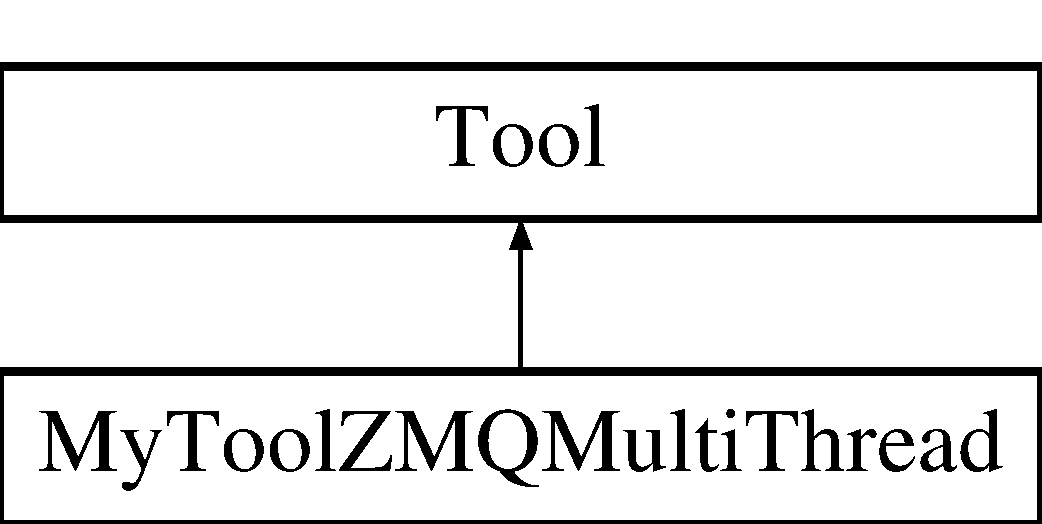
\includegraphics[height=2.000000cm]{classMyToolZMQMultiThread}
\end{center}
\end{figure}
\subsection*{Public Member Functions}
\begin{DoxyCompactItemize}
\item 
\hypertarget{classMyToolZMQMultiThread_a4036001006932887c7ed36eda1d1af50}{\hyperlink{classMyToolZMQMultiThread_a4036001006932887c7ed36eda1d1af50}{My\-Tool\-Z\-M\-Q\-Multi\-Thread} ()}\label{classMyToolZMQMultiThread_a4036001006932887c7ed36eda1d1af50}

\begin{DoxyCompactList}\small\item\em Simple constructor. \end{DoxyCompactList}\item 
bool \hyperlink{classMyToolZMQMultiThread_a99c3814d25f3868c5287f314bb63281d}{Initialise} (std\-::string configfile, \hyperlink{classDataModel}{Data\-Model} \&data)
\begin{DoxyCompactList}\small\item\em Initialise Function for setting up Tool resorces. \end{DoxyCompactList}\item 
\hypertarget{classMyToolZMQMultiThread_a15dea77298aa4c4b0e8a5cbbd244df28}{bool \hyperlink{classMyToolZMQMultiThread_a15dea77298aa4c4b0e8a5cbbd244df28}{Execute} ()}\label{classMyToolZMQMultiThread_a15dea77298aa4c4b0e8a5cbbd244df28}

\begin{DoxyCompactList}\small\item\em Executre function used to perform Tool perpose. \end{DoxyCompactList}\item 
\hypertarget{classMyToolZMQMultiThread_a4a7d1462aa1f6ea790be76161267547d}{bool \hyperlink{classMyToolZMQMultiThread_a4a7d1462aa1f6ea790be76161267547d}{Finalise} ()}\label{classMyToolZMQMultiThread_a4a7d1462aa1f6ea790be76161267547d}

\begin{DoxyCompactList}\small\item\em Finalise funciton used to clean up resorces. \end{DoxyCompactList}\end{DoxyCompactItemize}


\subsection{Detailed Description}
This is a template for a Tool that provides multiple worker threads and comunicates with them via Z\-M\-Q in a thread safe way. Please fill out the descripton and author information.

\begin{DoxyParagraph}{Author\-:}
B.\-Richards 
\end{DoxyParagraph}
\begin{DoxyParagraph}{Date\-:}
2019/05/28 10\-:44\-:00 
\end{DoxyParagraph}
Contact\-: \href{mailto:b.richards@qmul.ac.uk}{\tt b.\-richards@qmul.\-ac.\-uk} 

\subsection{Member Function Documentation}
\hypertarget{classMyToolZMQMultiThread_a99c3814d25f3868c5287f314bb63281d}{\index{My\-Tool\-Z\-M\-Q\-Multi\-Thread@{My\-Tool\-Z\-M\-Q\-Multi\-Thread}!Initialise@{Initialise}}
\index{Initialise@{Initialise}!MyToolZMQMultiThread@{My\-Tool\-Z\-M\-Q\-Multi\-Thread}}
\subsubsection[{Initialise}]{\setlength{\rightskip}{0pt plus 5cm}bool My\-Tool\-Z\-M\-Q\-Multi\-Thread\-::\-Initialise (
\begin{DoxyParamCaption}
\item[{std\-::string}]{configfile, }
\item[{{\bf Data\-Model} \&}]{data}
\end{DoxyParamCaption}
)}}\label{classMyToolZMQMultiThread_a99c3814d25f3868c5287f314bb63281d}


Initialise Function for setting up Tool resorces. 


\begin{DoxyParams}{Parameters}
{\em configfile} & The path and name of the dynamic configuration file to read in. \\
\hline
{\em data} & A reference to the transient data class used to pass information between Tools. \\
\hline
\end{DoxyParams}


The documentation for this class was generated from the following files\-:\begin{DoxyCompactItemize}
\item 
User\-Tools/template/My\-Tool\-Z\-M\-Q\-Multi\-Thread.\-h\item 
User\-Tools/template/My\-Tool\-Z\-M\-Q\-Multi\-Thread.\-cpp\end{DoxyCompactItemize}

\hypertarget{structMyToolZMQMultiThread__args}{\section{My\-Tool\-Z\-M\-Q\-Multi\-Thread\-\_\-args Struct Reference}
\label{structMyToolZMQMultiThread__args}\index{My\-Tool\-Z\-M\-Q\-Multi\-Thread\-\_\-args@{My\-Tool\-Z\-M\-Q\-Multi\-Thread\-\_\-args}}
}
Inheritance diagram for My\-Tool\-Z\-M\-Q\-Multi\-Thread\-\_\-args\-:\begin{figure}[H]
\begin{center}
\leavevmode
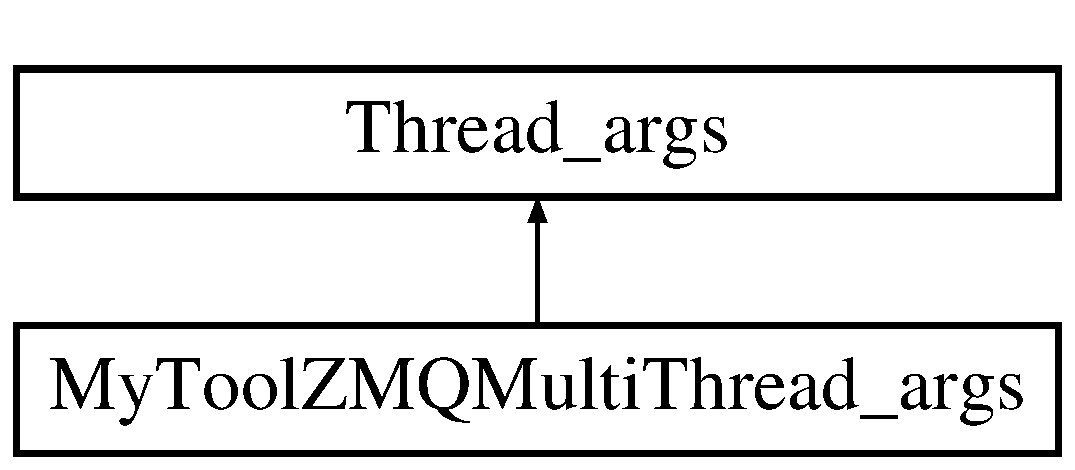
\includegraphics[height=2.000000cm]{structMyToolZMQMultiThread__args}
\end{center}
\end{figure}
\subsection*{Additional Inherited Members}


The documentation for this struct was generated from the following files\-:\begin{DoxyCompactItemize}
\item 
User\-Tools/template/My\-Tool\-Z\-M\-Q\-Multi\-Thread.\-h\item 
User\-Tools/template/My\-Tool\-Z\-M\-Q\-Multi\-Thread.\-cpp\end{DoxyCompactItemize}

\hypertarget{classNHits}{\section{N\-Hits Class Reference}
\label{classNHits}\index{N\-Hits@{N\-Hits}}
}
Inheritance diagram for N\-Hits\-:\begin{figure}[H]
\begin{center}
\leavevmode
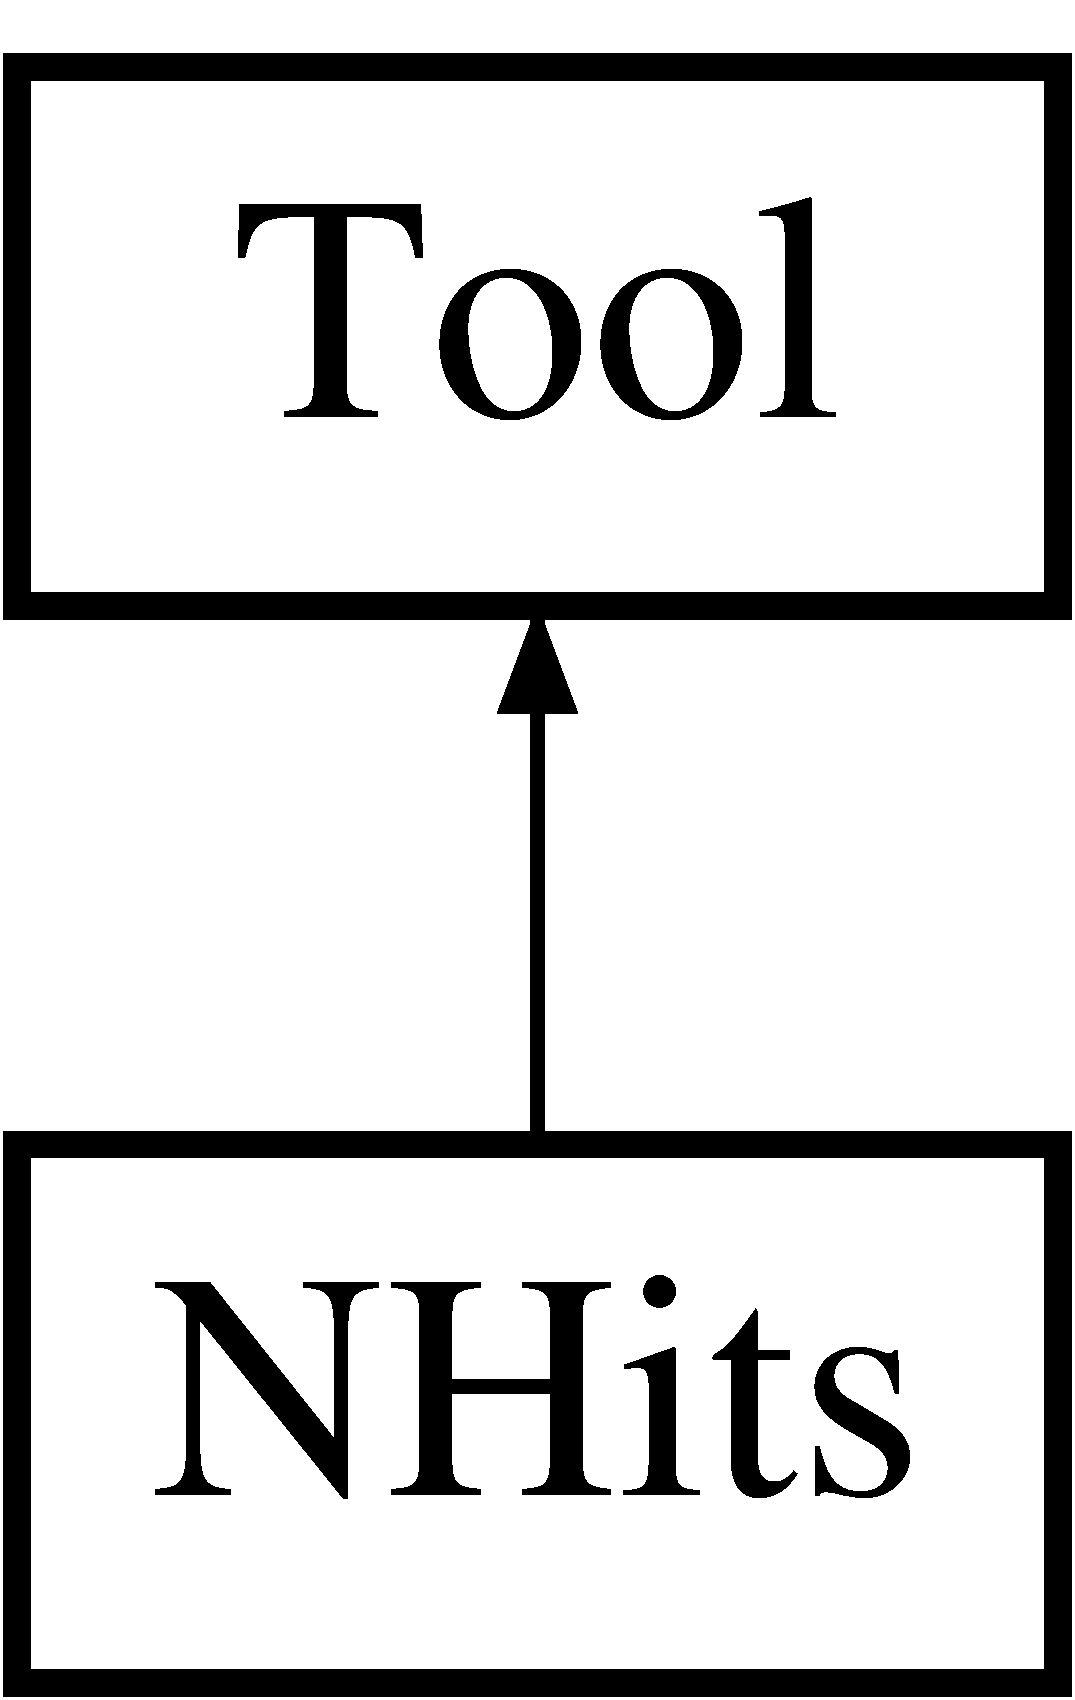
\includegraphics[height=2.000000cm]{classNHits}
\end{center}
\end{figure}
\subsection*{Public Member Functions}
\begin{DoxyCompactItemize}
\item 
\hypertarget{classNHits_abd81c3cb8af1593906acf093df2c183a}{bool {\bfseries Initialise} (std\-::string configfile, \hyperlink{classDataModel}{Data\-Model} \&data)}\label{classNHits_abd81c3cb8af1593906acf093df2c183a}

\item 
\hypertarget{classNHits_a173075c07d7b02639dbf9a3d3f284a3e}{bool {\bfseries Execute} ()}\label{classNHits_a173075c07d7b02639dbf9a3d3f284a3e}

\item 
\hypertarget{classNHits_aa7abae011ccead326f565f7781845a3f}{bool {\bfseries Finalise} ()}\label{classNHits_aa7abae011ccead326f565f7781845a3f}

\end{DoxyCompactItemize}


The documentation for this class was generated from the following files\-:\begin{DoxyCompactItemize}
\item 
User\-Tools/nhits/nhits.\-h\item 
User\-Tools/nhits/nhits.\-cpp\end{DoxyCompactItemize}

\hypertarget{classpass__all}{\section{pass\-\_\-all Class Reference}
\label{classpass__all}\index{pass\-\_\-all@{pass\-\_\-all}}
}
Inheritance diagram for pass\-\_\-all\-:\begin{figure}[H]
\begin{center}
\leavevmode
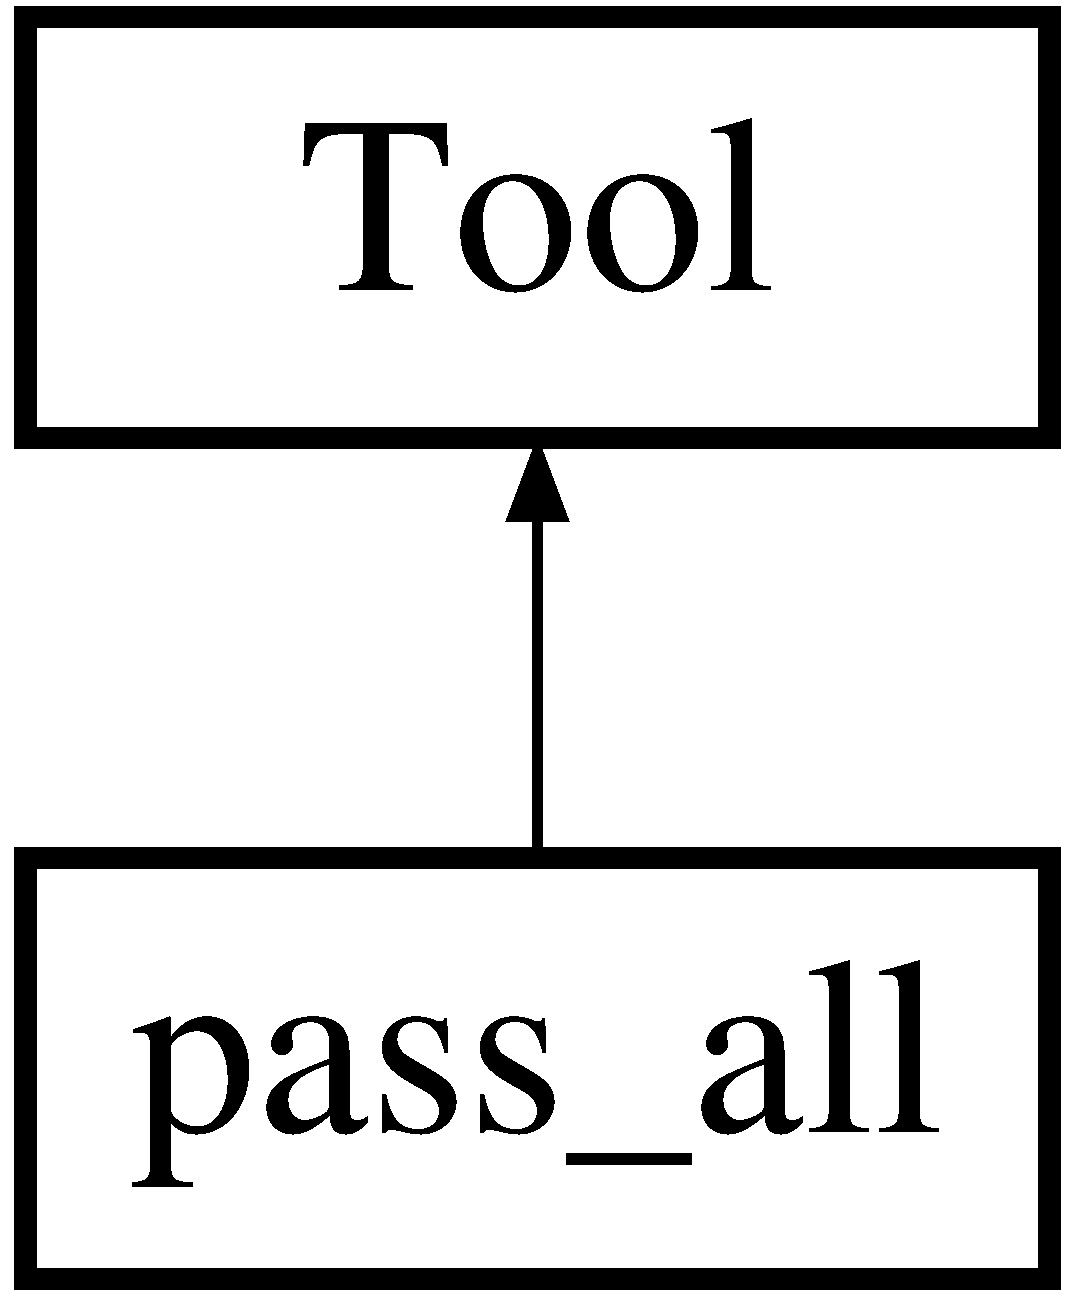
\includegraphics[height=2.000000cm]{classpass__all}
\end{center}
\end{figure}
\subsection*{Public Member Functions}
\begin{DoxyCompactItemize}
\item 
\hypertarget{classpass__all_aefc15a275cba8b1ce1c20d20505b03a6}{bool {\bfseries Initialise} (std\-::string configfile, \hyperlink{classDataModel}{Data\-Model} \&data)}\label{classpass__all_aefc15a275cba8b1ce1c20d20505b03a6}

\item 
\hypertarget{classpass__all_a734b577abe84ae81305705bd1125bc42}{bool {\bfseries Execute} ()}\label{classpass__all_a734b577abe84ae81305705bd1125bc42}

\item 
\hypertarget{classpass__all_a272302f6e0c6bfa737d18124665b540c}{bool {\bfseries Finalise} ()}\label{classpass__all_a272302f6e0c6bfa737d18124665b540c}

\end{DoxyCompactItemize}


The documentation for this class was generated from the following files\-:\begin{DoxyCompactItemize}
\item 
User\-Tools/pass\-\_\-all/pass\-\_\-all.\-h\item 
User\-Tools/pass\-\_\-all/pass\-\_\-all.\-cpp\end{DoxyCompactItemize}

\hypertarget{classPMTInfo}{\section{P\-M\-T\-Info Class Reference}
\label{classPMTInfo}\index{P\-M\-T\-Info@{P\-M\-T\-Info}}
}
\subsection*{Public Member Functions}
\begin{DoxyCompactItemize}
\item 
\hypertarget{classPMTInfo_a46318641774fe21018e07b4416f2648e}{{\bfseries P\-M\-T\-Info} (int tubeno, float x, float y, float z)}\label{classPMTInfo_a46318641774fe21018e07b4416f2648e}

\end{DoxyCompactItemize}
\subsection*{Public Attributes}
\begin{DoxyCompactItemize}
\item 
\hypertarget{classPMTInfo_a573f237c93ab1e7e6949a4f70d63f49e}{int {\bfseries m\-\_\-tubeno}}\label{classPMTInfo_a573f237c93ab1e7e6949a4f70d63f49e}

\item 
\hypertarget{classPMTInfo_ad6c7d488f214e32d0f8ce68785238c8e}{float {\bfseries m\-\_\-x}}\label{classPMTInfo_ad6c7d488f214e32d0f8ce68785238c8e}

\item 
\hypertarget{classPMTInfo_aed9a6e7cd9a1caa2fcaeceb861898e0f}{float {\bfseries m\-\_\-y}}\label{classPMTInfo_aed9a6e7cd9a1caa2fcaeceb861898e0f}

\item 
\hypertarget{classPMTInfo_aff95f0c2b0dfaa30262c82cc5eb17a06}{float {\bfseries m\-\_\-z}}\label{classPMTInfo_aff95f0c2b0dfaa30262c82cc5eb17a06}

\end{DoxyCompactItemize}


The documentation for this class was generated from the following files\-:\begin{DoxyCompactItemize}
\item 
Data\-Model/P\-M\-T\-Info.\-h\item 
Data\-Model/P\-M\-T\-Info.\-cpp\end{DoxyCompactItemize}

\hypertarget{structPos3D}{\section{Pos3\-D Struct Reference}
\label{structPos3D}\index{Pos3\-D@{Pos3\-D}}
}
\subsection*{Public Member Functions}
\begin{DoxyCompactItemize}
\item 
\hypertarget{structPos3D_a558c147eba6079b4e24a4e864f6bd888}{double {\bfseries R} ()}\label{structPos3D_a558c147eba6079b4e24a4e864f6bd888}

\end{DoxyCompactItemize}
\subsection*{Public Attributes}
\begin{DoxyCompactItemize}
\item 
\hypertarget{structPos3D_af72360d7df47870e345011dcddcf9c7c}{double {\bfseries x}}\label{structPos3D_af72360d7df47870e345011dcddcf9c7c}

\item 
\hypertarget{structPos3D_a6e538472b536e07f3f2825ef7f912e88}{double {\bfseries y}}\label{structPos3D_a6e538472b536e07f3f2825ef7f912e88}

\item 
\hypertarget{structPos3D_a6b26b787c2b9774956bb8236404e11a3}{double {\bfseries z}}\label{structPos3D_a6b26b787c2b9774956bb8236404e11a3}

\end{DoxyCompactItemize}


The documentation for this struct was generated from the following file\-:\begin{DoxyCompactItemize}
\item 
Data\-Model/Recon\-Info.\-h\end{DoxyCompactItemize}

\hypertarget{classPrepareSubSamples}{\section{Prepare\-Sub\-Samples Class Reference}
\label{classPrepareSubSamples}\index{Prepare\-Sub\-Samples@{Prepare\-Sub\-Samples}}
}
Inheritance diagram for Prepare\-Sub\-Samples\-:\begin{figure}[H]
\begin{center}
\leavevmode
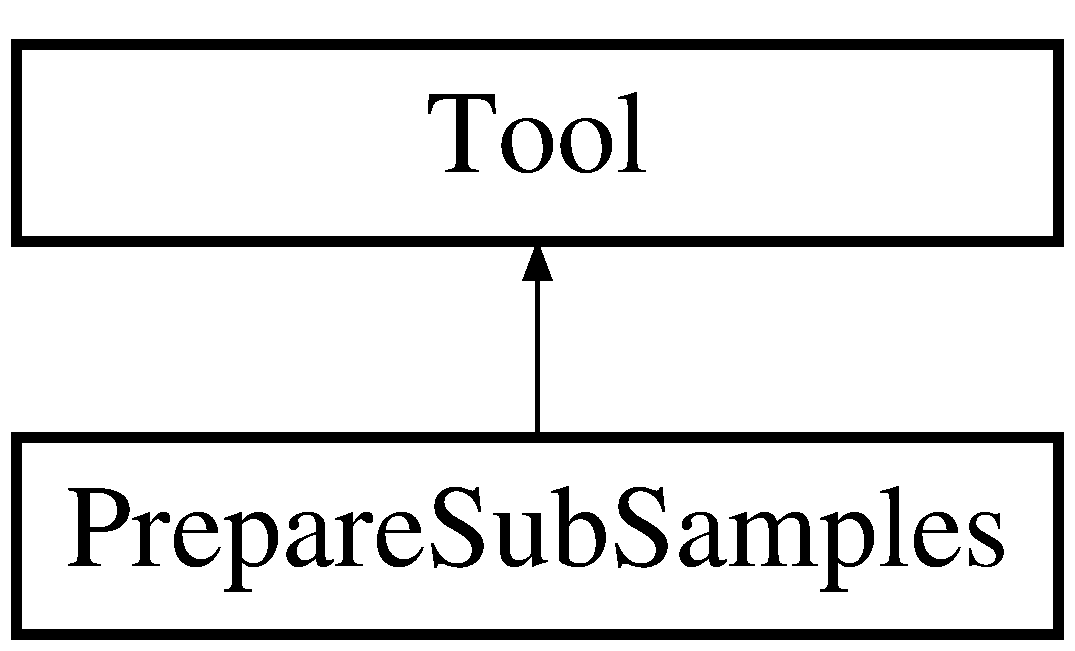
\includegraphics[height=2.000000cm]{classPrepareSubSamples}
\end{center}
\end{figure}
\subsection*{Public Member Functions}
\begin{DoxyCompactItemize}
\item 
\hypertarget{classPrepareSubSamples_a8d85a66ab8377637756e2fe5580b0578}{bool {\bfseries Initialise} (std\-::string configfile, \hyperlink{classDataModel}{Data\-Model} \&data)}\label{classPrepareSubSamples_a8d85a66ab8377637756e2fe5580b0578}

\item 
\hypertarget{classPrepareSubSamples_a952b1bbc3a74ae7ec0f45b8700e0f918}{bool {\bfseries Execute} ()}\label{classPrepareSubSamples_a952b1bbc3a74ae7ec0f45b8700e0f918}

\item 
\hypertarget{classPrepareSubSamples_ad13127e510e00b6b3898f3e39ca0a4aa}{bool {\bfseries Finalise} ()}\label{classPrepareSubSamples_ad13127e510e00b6b3898f3e39ca0a4aa}

\end{DoxyCompactItemize}


The documentation for this class was generated from the following files\-:\begin{DoxyCompactItemize}
\item 
User\-Tools/\-Prepare\-Sub\-Samples/Prepare\-Sub\-Samples.\-h\item 
User\-Tools/\-Prepare\-Sub\-Samples/Prepare\-Sub\-Samples.\-cpp\end{DoxyCompactItemize}

\hypertarget{classReconDataIn}{\section{Recon\-Data\-In Class Reference}
\label{classReconDataIn}\index{Recon\-Data\-In@{Recon\-Data\-In}}
}
Inheritance diagram for Recon\-Data\-In\-:\begin{figure}[H]
\begin{center}
\leavevmode
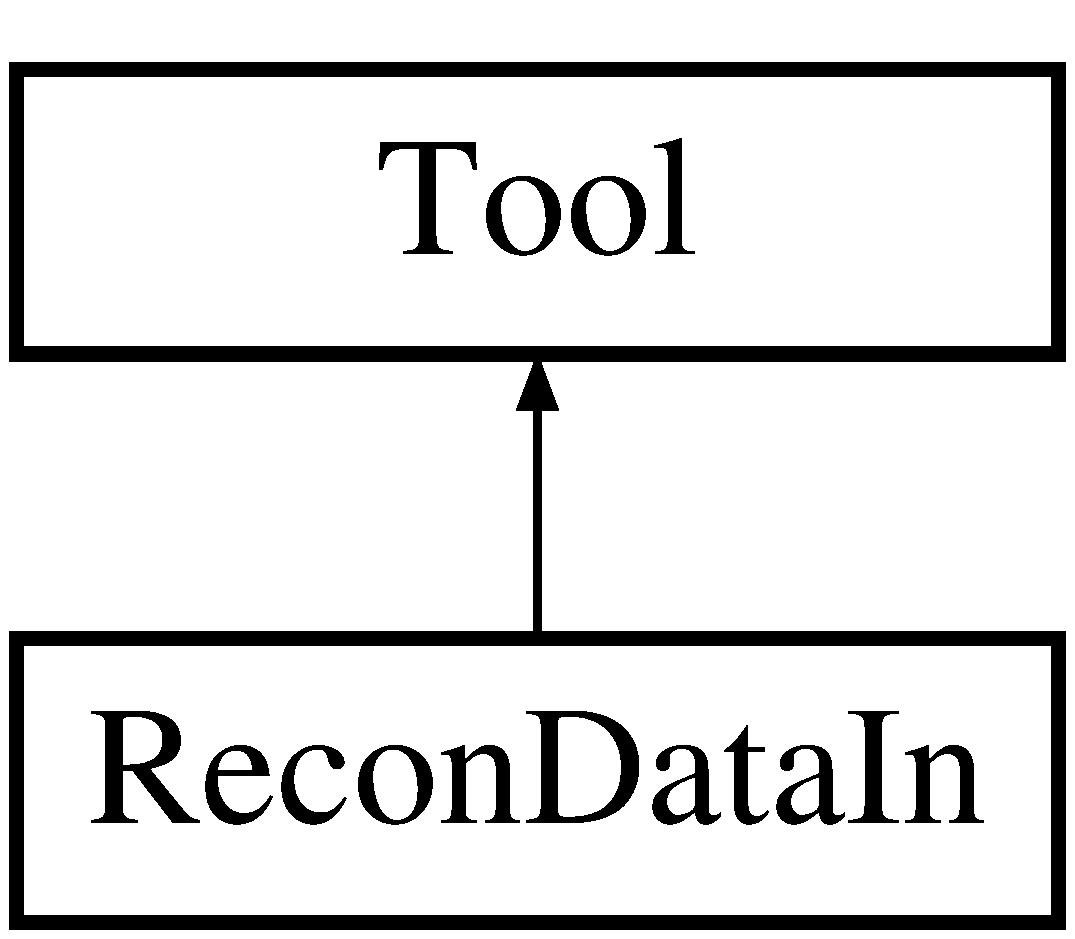
\includegraphics[height=2.000000cm]{classReconDataIn}
\end{center}
\end{figure}
\subsection*{Public Member Functions}
\begin{DoxyCompactItemize}
\item 
\hypertarget{classReconDataIn_a6f79d79fbeeeeade6f5eac8168fcce48}{bool {\bfseries Initialise} (std\-::string configfile, \hyperlink{classDataModel}{Data\-Model} \&data)}\label{classReconDataIn_a6f79d79fbeeeeade6f5eac8168fcce48}

\item 
\hypertarget{classReconDataIn_a54462fd9d4309f25a5a504bbc2ebeefb}{bool {\bfseries Execute} ()}\label{classReconDataIn_a54462fd9d4309f25a5a504bbc2ebeefb}

\item 
\hypertarget{classReconDataIn_abc3026b2188e32436d37d461f702809a}{bool {\bfseries Finalise} ()}\label{classReconDataIn_abc3026b2188e32436d37d461f702809a}

\end{DoxyCompactItemize}


The documentation for this class was generated from the following files\-:\begin{DoxyCompactItemize}
\item 
User\-Tools/\-Recon\-Data\-In/Recon\-Data\-In.\-h\item 
User\-Tools/\-Recon\-Data\-In/Recon\-Data\-In.\-cpp\end{DoxyCompactItemize}

\hypertarget{classReconDataOut}{\section{Recon\-Data\-Out Class Reference}
\label{classReconDataOut}\index{Recon\-Data\-Out@{Recon\-Data\-Out}}
}
Inheritance diagram for Recon\-Data\-Out\-:\begin{figure}[H]
\begin{center}
\leavevmode
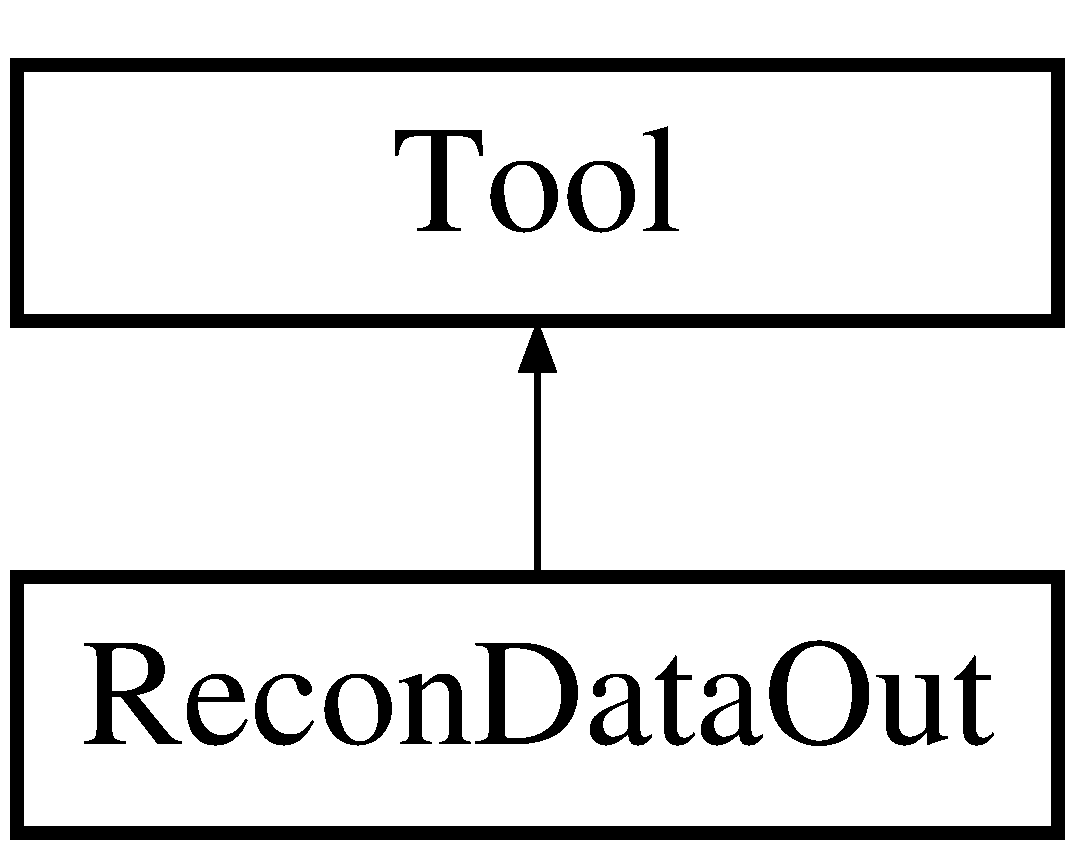
\includegraphics[height=2.000000cm]{classReconDataOut}
\end{center}
\end{figure}
\subsection*{Public Member Functions}
\begin{DoxyCompactItemize}
\item 
\hypertarget{classReconDataOut_ae03522cbdf98cd524240adbfe3eb93c1}{bool {\bfseries Initialise} (std\-::string configfile, \hyperlink{classDataModel}{Data\-Model} \&data)}\label{classReconDataOut_ae03522cbdf98cd524240adbfe3eb93c1}

\item 
\hypertarget{classReconDataOut_a1977f763aac394aba4099f45e4d567b0}{bool {\bfseries Execute} ()}\label{classReconDataOut_a1977f763aac394aba4099f45e4d567b0}

\item 
\hypertarget{classReconDataOut_a0b00ffbbabc530228b32aa26eab859f6}{bool {\bfseries Finalise} ()}\label{classReconDataOut_a0b00ffbbabc530228b32aa26eab859f6}

\end{DoxyCompactItemize}


The documentation for this class was generated from the following files\-:\begin{DoxyCompactItemize}
\item 
User\-Tools/\-Recon\-Data\-Out/Recon\-Data\-Out.\-h\item 
User\-Tools/\-Recon\-Data\-Out/Recon\-Data\-Out.\-cpp\end{DoxyCompactItemize}

\hypertarget{classReconFilter}{\section{Recon\-Filter Class Reference}
\label{classReconFilter}\index{Recon\-Filter@{Recon\-Filter}}
}
Inheritance diagram for Recon\-Filter\-:\begin{figure}[H]
\begin{center}
\leavevmode
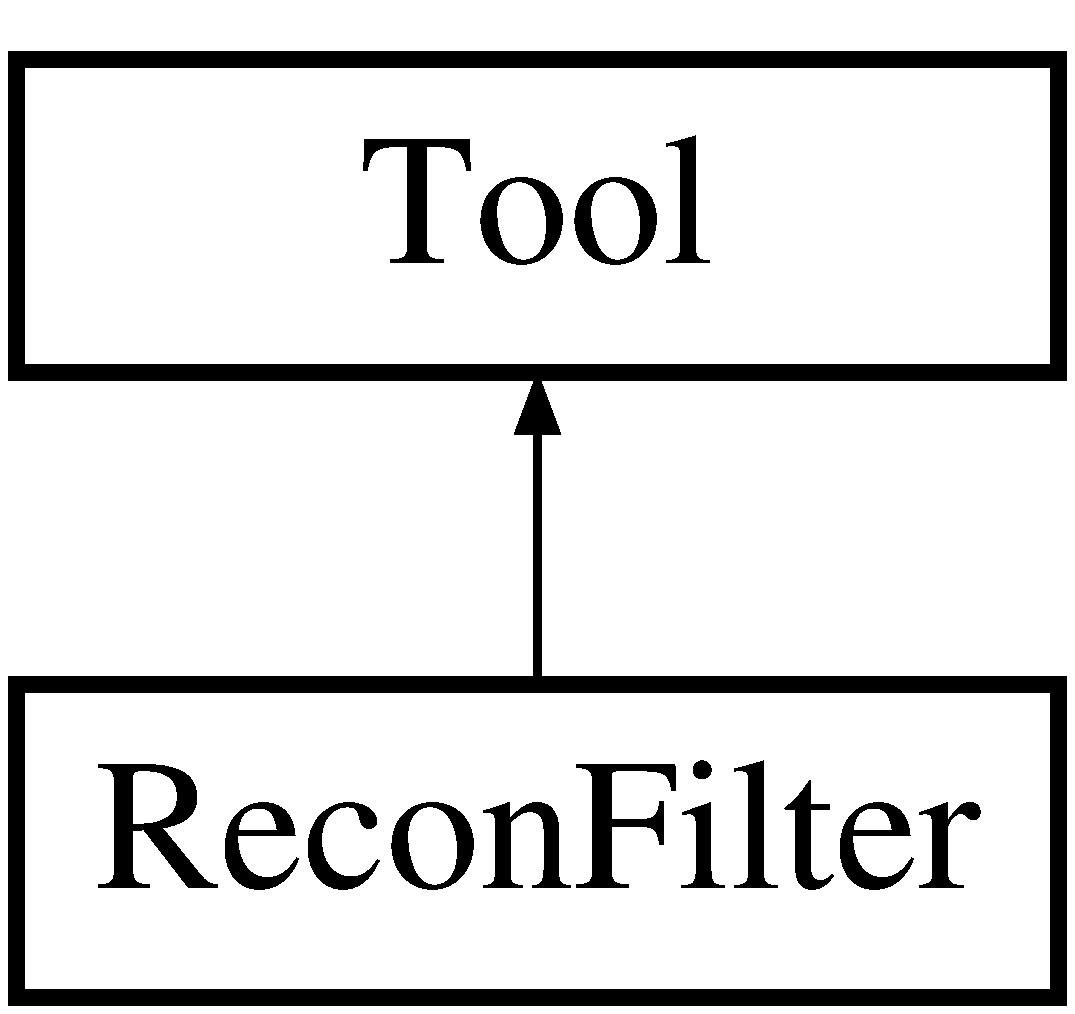
\includegraphics[height=2.000000cm]{classReconFilter}
\end{center}
\end{figure}
\subsection*{Public Member Functions}
\begin{DoxyCompactItemize}
\item 
\hypertarget{classReconFilter_acdcfc0da11326a8eef6abdbabe875370}{bool {\bfseries Initialise} (std\-::string configfile, \hyperlink{classDataModel}{Data\-Model} \&data)}\label{classReconFilter_acdcfc0da11326a8eef6abdbabe875370}

\item 
\hypertarget{classReconFilter_aab5a05ec6308957aa6197ea698589b5e}{bool {\bfseries Execute} ()}\label{classReconFilter_aab5a05ec6308957aa6197ea698589b5e}

\item 
\hypertarget{classReconFilter_af167ee66ac9dbb412bf0954be8046ef4}{bool {\bfseries Finalise} ()}\label{classReconFilter_af167ee66ac9dbb412bf0954be8046ef4}

\end{DoxyCompactItemize}


The documentation for this class was generated from the following files\-:\begin{DoxyCompactItemize}
\item 
User\-Tools/\-Recon\-Filter/Recon\-Filter.\-h\item 
User\-Tools/\-Recon\-Filter/Recon\-Filter.\-cpp\end{DoxyCompactItemize}

\hypertarget{classReconInfo}{\section{Recon\-Info Class Reference}
\label{classReconInfo}\index{Recon\-Info@{Recon\-Info}}
}
\subsection*{Public Member Functions}
\begin{DoxyCompactItemize}
\item 
\hypertarget{classReconInfo_af15bf0a0673c3ba6a18423e0357bd95b}{void {\bfseries Add\-Recon} (Reconstructer\-\_\-t reconstructer, int trigger\-\_\-num, int nhits, \hyperlink{classTimeDelta}{Time\-Delta} time, double $\ast$vertex, double goodness\-\_\-of\-\_\-fit, double goodness\-\_\-of\-\_\-time\-\_\-fit, bool fill\-\_\-has\-\_\-direction=true, double energy=-\/1.)}\label{classReconInfo_af15bf0a0673c3ba6a18423e0357bd95b}

\item 
\hypertarget{classReconInfo_acf71ac70ce0587d31d3040d35bf50b51}{void {\bfseries Add\-Recon} (Reconstructer\-\_\-t reconstructer, int trigger\-\_\-num, int nhits, \hyperlink{classTimeDelta}{Time\-Delta} time, double $\ast$vertex, double goodness\-\_\-of\-\_\-fit, double goodness\-\_\-of\-\_\-time\-\_\-fit, double $\ast$direction\-\_\-euler, double $\ast$cherenkov\-\_\-cone, double direction\-\_\-likelihood, double energy=-\/1.)}\label{classReconInfo_acf71ac70ce0587d31d3040d35bf50b51}

\item 
\hypertarget{classReconInfo_a96c16b9d66349d7eed2e4ada1c40525c}{void {\bfseries Add\-Recon\-From} (\hyperlink{classReconInfo}{Recon\-Info} $\ast$in, const int irecon)}\label{classReconInfo_a96c16b9d66349d7eed2e4ada1c40525c}

\item 
\hypertarget{classReconInfo_a2a9e7b5d70ab362de7d34217d15310dc}{int {\bfseries Get\-N\-Recons} ()}\label{classReconInfo_a2a9e7b5d70ab362de7d34217d15310dc}

\item 
\hypertarget{classReconInfo_ab515ad33a974ea715d0b4cb5edf101f9}{\hyperlink{classTimeDelta}{Time\-Delta} {\bfseries Get\-First\-Time} ()}\label{classReconInfo_ab515ad33a974ea715d0b4cb5edf101f9}

\item 
\hypertarget{classReconInfo_ac9a0283e1c4a62135793c256d48bf99d}{\hyperlink{classTimeDelta}{Time\-Delta} {\bfseries Get\-Last\-Time} ()}\label{classReconInfo_ac9a0283e1c4a62135793c256d48bf99d}

\item 
\hypertarget{classReconInfo_a4cbe5c22fdb5ccb337e91b636770c8d8}{Reconstructer\-\_\-t {\bfseries Get\-Reconstructer} (int irecon)}\label{classReconInfo_a4cbe5c22fdb5ccb337e91b636770c8d8}

\item 
\hypertarget{classReconInfo_a6bf88674ba47e30e004ec39179806575}{int {\bfseries Get\-Trigger\-Num} (int irecon)}\label{classReconInfo_a6bf88674ba47e30e004ec39179806575}

\item 
\hypertarget{classReconInfo_a9e34f7e22595b583f6b70749cf3321b6}{int {\bfseries Get\-N\-Hits} (int irecon)}\label{classReconInfo_a9e34f7e22595b583f6b70749cf3321b6}

\item 
\hypertarget{classReconInfo_ac19bad0f4af4dabb4e8517181f670795}{double {\bfseries Get\-Energy} (int irecon)}\label{classReconInfo_ac19bad0f4af4dabb4e8517181f670795}

\item 
\hypertarget{classReconInfo_ae54737e4ec00e103cfd214dafa6b6313}{void {\bfseries Set\-Energy} (int irecon, double energy)}\label{classReconInfo_ae54737e4ec00e103cfd214dafa6b6313}

\item 
\hypertarget{classReconInfo_ac98f1d0a6be5e2ae54ea209022bad403}{\hyperlink{classTimeDelta}{Time\-Delta} {\bfseries Get\-Time} (int irecon)}\label{classReconInfo_ac98f1d0a6be5e2ae54ea209022bad403}

\item 
\hypertarget{classReconInfo_a3b0e7457d82ba538556e377e5a67ebe2}{\hyperlink{structPos3D}{Pos3\-D} {\bfseries Get\-Vertex} (int irecon)}\label{classReconInfo_a3b0e7457d82ba538556e377e5a67ebe2}

\item 
\hypertarget{classReconInfo_a62fdfb94f15d32711fb78db2dfdf8c84}{double {\bfseries Get\-Goodness\-Of\-Fit} (int irecon)}\label{classReconInfo_a62fdfb94f15d32711fb78db2dfdf8c84}

\item 
\hypertarget{classReconInfo_a453dae55666b27b10a8d13aba3112b93}{double {\bfseries Get\-Goodness\-Of\-Time\-Fit} (int irecon)}\label{classReconInfo_a453dae55666b27b10a8d13aba3112b93}

\item 
\hypertarget{classReconInfo_ac4f154d184b7645943955f507281672e}{bool {\bfseries Get\-Has\-Direction} (int irecon)}\label{classReconInfo_ac4f154d184b7645943955f507281672e}

\item 
\hypertarget{classReconInfo_aace0a3e60fd49fbb5ef7a0a14afbd934}{\hyperlink{structDirectionEuler}{Direction\-Euler} {\bfseries Get\-Direction\-Euler} (int irecon)}\label{classReconInfo_aace0a3e60fd49fbb5ef7a0a14afbd934}

\item 
\hypertarget{classReconInfo_a98857e740b0c84d05a350a375ab00aab}{\hyperlink{structCherenkovCone}{Cherenkov\-Cone} {\bfseries Get\-Cherenkov\-Cone} (int irecon)}\label{classReconInfo_a98857e740b0c84d05a350a375ab00aab}

\item 
\hypertarget{classReconInfo_a8fd62e5800e1dfd8b4fbb73db36c6c80}{double {\bfseries Get\-Direction\-Likelihood} (int irecon)}\label{classReconInfo_a8fd62e5800e1dfd8b4fbb73db36c6c80}

\item 
\hypertarget{classReconInfo_a011aa23ea6b1dcc430b107d89faa24b0}{void {\bfseries Reset} ()}\label{classReconInfo_a011aa23ea6b1dcc430b107d89faa24b0}

\end{DoxyCompactItemize}
\subsection*{Static Public Member Functions}
\begin{DoxyCompactItemize}
\item 
\hypertarget{classReconInfo_ac3f741957faf5a7d1c3d21bff107e12a}{static std\-::string {\bfseries Enum\-As\-String} (Reconstructer\-\_\-t r)}\label{classReconInfo_ac3f741957faf5a7d1c3d21bff107e12a}

\item 
\hypertarget{classReconInfo_a76cff9cb354ff64edee198be5339a40e}{static Reconstructer\-\_\-t {\bfseries Reconstructer\-From\-String} (std\-::string s)}\label{classReconInfo_a76cff9cb354ff64edee198be5339a40e}

\item 
\hypertarget{classReconInfo_aa2b43e35c45992db11f8809384602853}{static std\-::string {\bfseries Enum\-As\-String} (N\-Clusters\-Warning\-\_\-t w)}\label{classReconInfo_aa2b43e35c45992db11f8809384602853}

\item 
\hypertarget{classReconInfo_a2f307a0fdbd190822a0377a011c9d379}{static N\-Clusters\-Warning\-\_\-t {\bfseries N\-Clusters\-Warning\-From\-String} (std\-::string s)}\label{classReconInfo_a2f307a0fdbd190822a0377a011c9d379}

\item 
\hypertarget{classReconInfo_a82fd1058a8c3f23498671fcacc96d819}{static std\-::string {\bfseries Enum\-As\-String} (S\-N\-Warning\-\_\-t w)}\label{classReconInfo_a82fd1058a8c3f23498671fcacc96d819}

\item 
\hypertarget{classReconInfo_a498702bd5e2e496f872976f14853b8ea}{static S\-N\-Warning\-\_\-t {\bfseries S\-N\-Warning\-From\-String} (std\-::string s)}\label{classReconInfo_a498702bd5e2e496f872976f14853b8ea}

\item 
\hypertarget{classReconInfo_a9d68ec13cb242350f97d30b7d9257ab4}{static bool {\bfseries Should\-Provide\-Direction} (Reconstructer\-\_\-t r)}\label{classReconInfo_a9d68ec13cb242350f97d30b7d9257ab4}

\end{DoxyCompactItemize}


The documentation for this class was generated from the following files\-:\begin{DoxyCompactItemize}
\item 
Data\-Model/Recon\-Info.\-h\item 
Data\-Model/Recon\-Info.\-cpp\end{DoxyCompactItemize}

\hypertarget{classReconRandomiser}{\section{Recon\-Randomiser Class Reference}
\label{classReconRandomiser}\index{Recon\-Randomiser@{Recon\-Randomiser}}
}
Inheritance diagram for Recon\-Randomiser\-:\begin{figure}[H]
\begin{center}
\leavevmode
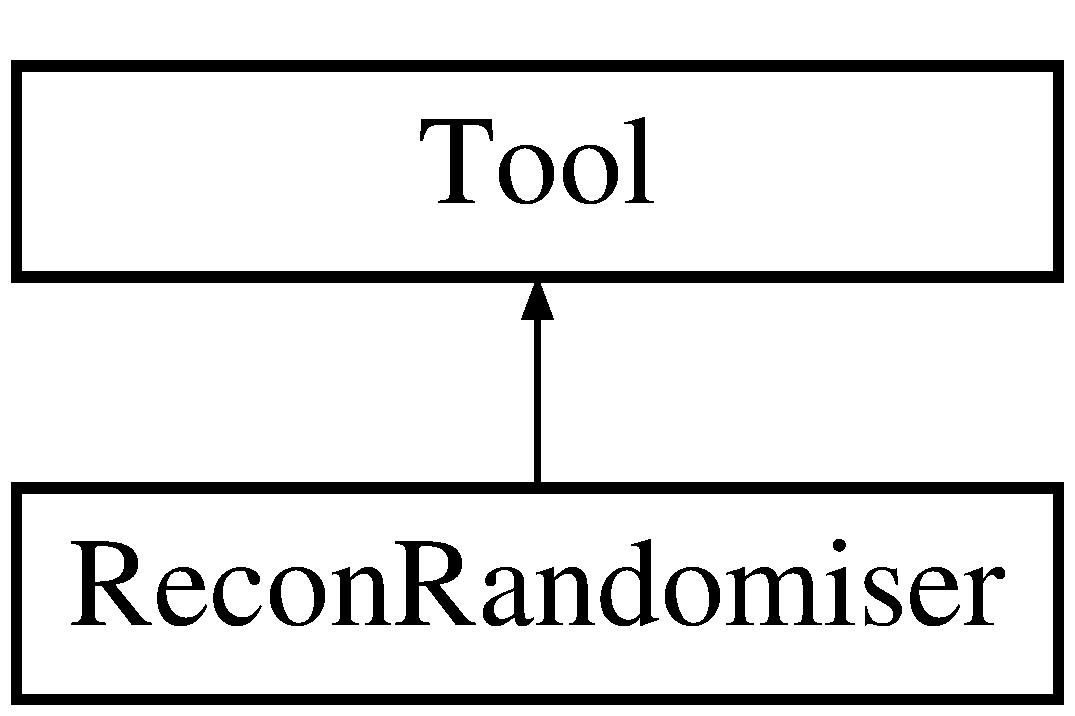
\includegraphics[height=2.000000cm]{classReconRandomiser}
\end{center}
\end{figure}
\subsection*{Public Member Functions}
\begin{DoxyCompactItemize}
\item 
\hypertarget{classReconRandomiser_a5fcdae68a66b1a1988b36cc9224d63e2}{bool {\bfseries Initialise} (std\-::string configfile, \hyperlink{classDataModel}{Data\-Model} \&data)}\label{classReconRandomiser_a5fcdae68a66b1a1988b36cc9224d63e2}

\item 
\hypertarget{classReconRandomiser_a45093e181c6a60ee31efafba3a11e676}{bool {\bfseries Execute} ()}\label{classReconRandomiser_a45093e181c6a60ee31efafba3a11e676}

\item 
\hypertarget{classReconRandomiser_a9376c492952fac4d5ff59f1c57a4cee7}{bool {\bfseries Finalise} ()}\label{classReconRandomiser_a9376c492952fac4d5ff59f1c57a4cee7}

\end{DoxyCompactItemize}


The documentation for this class was generated from the following files\-:\begin{DoxyCompactItemize}
\item 
User\-Tools/\-Recon\-Randomiser/Recon\-Randomiser.\-h\item 
User\-Tools/\-Recon\-Randomiser/Recon\-Randomiser.\-cpp\end{DoxyCompactItemize}

\hypertarget{classReconReset}{\section{Recon\-Reset Class Reference}
\label{classReconReset}\index{Recon\-Reset@{Recon\-Reset}}
}
Inheritance diagram for Recon\-Reset\-:\begin{figure}[H]
\begin{center}
\leavevmode
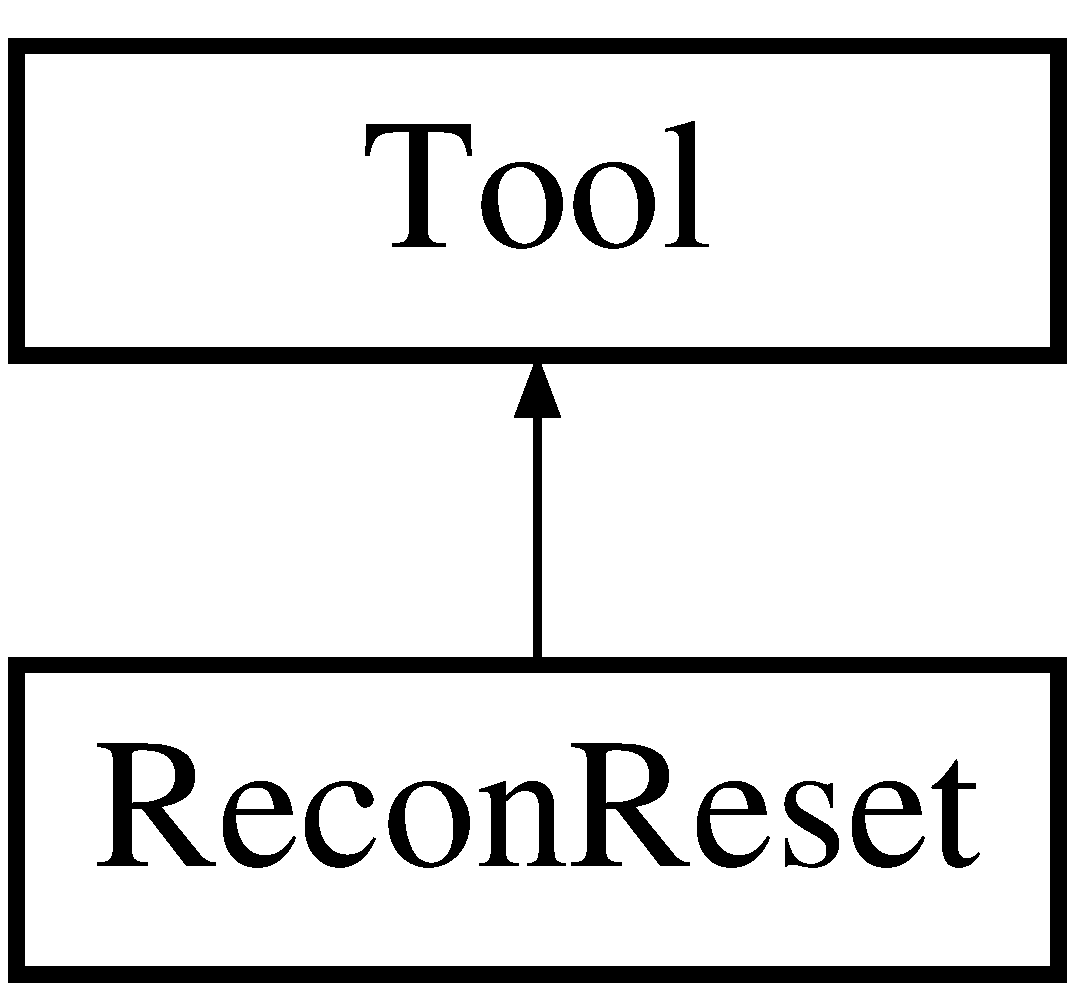
\includegraphics[height=2.000000cm]{classReconReset}
\end{center}
\end{figure}
\subsection*{Public Member Functions}
\begin{DoxyCompactItemize}
\item 
\hypertarget{classReconReset_af692157504b2a84938ccd651c8dbbd96}{bool {\bfseries Initialise} (std\-::string configfile, \hyperlink{classDataModel}{Data\-Model} \&data)}\label{classReconReset_af692157504b2a84938ccd651c8dbbd96}

\item 
\hypertarget{classReconReset_a299f661de185811285d6b5bedfeb8320}{bool {\bfseries Execute} ()}\label{classReconReset_a299f661de185811285d6b5bedfeb8320}

\item 
\hypertarget{classReconReset_a1f5f4c8170fee66f5f68609c88f85046}{bool {\bfseries Finalise} ()}\label{classReconReset_a1f5f4c8170fee66f5f68609c88f85046}

\end{DoxyCompactItemize}


The documentation for this class was generated from the following files\-:\begin{DoxyCompactItemize}
\item 
User\-Tools/\-Recon\-Reset/Recon\-Reset.\-h\item 
User\-Tools/\-Recon\-Reset/Recon\-Reset.\-cpp\end{DoxyCompactItemize}

\hypertarget{classSampleChunk}{\section{Sample\-Chunk Class Reference}
\label{classSampleChunk}\index{Sample\-Chunk@{Sample\-Chunk}}
}
\subsection*{Public Attributes}
\begin{DoxyCompactItemize}
\item 
\hypertarget{classSampleChunk_ae227f86f1e9602b555a59145fe34fc12}{std\-::vector$<$ int $>$ \hyperlink{classSampleChunk_ae227f86f1e9602b555a59145fe34fc12}{m\-\_\-\-P\-M\-Tid}}\label{classSampleChunk_ae227f86f1e9602b555a59145fe34fc12}

\begin{DoxyCompactList}\small\item\em Vector of P\-M\-T I\-Ds for all hits in \hyperlink{classSampleChunk}{Sample\-Chunk}. \end{DoxyCompactList}\item 
\hypertarget{classSampleChunk_a2fcaaeb44f8cc604e6cc2eeec268ec1c}{std\-::vector\\*
$<$ \hyperlink{classTimeDelta_afe4b7adde6a0645a8ada61f39e198c8e}{Time\-Delta\-::short\-\_\-time\-\_\-t} $>$ \hyperlink{classSampleChunk_a2fcaaeb44f8cc604e6cc2eeec268ec1c}{m\-\_\-time}}\label{classSampleChunk_a2fcaaeb44f8cc604e6cc2eeec268ec1c}

\begin{DoxyCompactList}\small\item\em Vector of hit times relative to timestamp for all hits in \hyperlink{classSampleChunk}{Sample\-Chunk}. Unit\-: ns. \end{DoxyCompactList}\item 
\hypertarget{classSampleChunk_a5540aa8a6f27b1a5b4accf80bb91a333}{std\-::vector$<$ float $>$ \hyperlink{classSampleChunk_a5540aa8a6f27b1a5b4accf80bb91a333}{m\-\_\-charge}}\label{classSampleChunk_a5540aa8a6f27b1a5b4accf80bb91a333}

\begin{DoxyCompactList}\small\item\em Vector of charges for all hits in \hyperlink{classSampleChunk}{Sample\-Chunk}. Unit\-: photoelectrons (M\-C), calibrated photoelectrons (data) \end{DoxyCompactList}\item 
\hypertarget{classSampleChunk_a726be76a9337f10e715dc078cbede121}{Boost\-Store {\bfseries output}}\label{classSampleChunk_a726be76a9337f10e715dc078cbede121}

\end{DoxyCompactItemize}


The documentation for this class was generated from the following files\-:\begin{DoxyCompactItemize}
\item 
Data\-Model/Sample\-Chunk.\-h\item 
Data\-Model/Sample\-Chunk.\-cpp\end{DoxyCompactItemize}

\hypertarget{structSNWarningParams}{\section{S\-N\-Warning\-Params Struct Reference}
\label{structSNWarningParams}\index{S\-N\-Warning\-Params@{S\-N\-Warning\-Params}}
}
\subsection*{Public Member Functions}
\begin{DoxyCompactItemize}
\item 
\hypertarget{structSNWarningParams_a08362f6e7b4010c81b511df679d38048}{{\bfseries S\-N\-Warning\-Params} (int nclusters, int dim, N\-Clusters\-Warning\-\_\-t nclusters\-\_\-warning)}\label{structSNWarningParams_a08362f6e7b4010c81b511df679d38048}

\end{DoxyCompactItemize}
\subsection*{Public Attributes}
\begin{DoxyCompactItemize}
\item 
\hypertarget{structSNWarningParams_adad4ce9981ee71145013e4c4e2016ff6}{int {\bfseries m\-\_\-dim}}\label{structSNWarningParams_adad4ce9981ee71145013e4c4e2016ff6}

\item 
\hypertarget{structSNWarningParams_ac39f2733df6abe5cde86faa3fe3e208f}{int {\bfseries m\-\_\-nclusters}}\label{structSNWarningParams_ac39f2733df6abe5cde86faa3fe3e208f}

\item 
\hypertarget{structSNWarningParams_a770c3bc2f109ce3e76363199218cfcf3}{N\-Clusters\-Warning\-\_\-t {\bfseries m\-\_\-nclusters\-\_\-warning}}\label{structSNWarningParams_a770c3bc2f109ce3e76363199218cfcf3}

\end{DoxyCompactItemize}


The documentation for this struct was generated from the following file\-:\begin{DoxyCompactItemize}
\item 
Data\-Model/Recon\-Info.\-h\end{DoxyCompactItemize}

\hypertarget{classutil_1_1Stopwatch}{\section{util\-:\-:Stopwatch Class Reference}
\label{classutil_1_1Stopwatch}\index{util\-::\-Stopwatch@{util\-::\-Stopwatch}}
}
\subsection*{Public Member Functions}
\begin{DoxyCompactItemize}
\item 
\hypertarget{classutil_1_1Stopwatch_af8055e6f405f2093127dcb08a33dd6ab}{{\bfseries Stopwatch} (const char $\ast$tool\-\_\-name)}\label{classutil_1_1Stopwatch_af8055e6f405f2093127dcb08a33dd6ab}

\item 
\hypertarget{classutil_1_1Stopwatch_aaf40a5394011e56a8a51e4b87467e556}{void \hyperlink{classutil_1_1Stopwatch_aaf40a5394011e56a8a51e4b87467e556}{Start} ()}\label{classutil_1_1Stopwatch_aaf40a5394011e56a8a51e4b87467e556}

\begin{DoxyCompactList}\small\item\em Start the stopwatch. \end{DoxyCompactList}\item 
\hypertarget{classutil_1_1Stopwatch_a0dbc5976e1bd883b0fcf382d6dd1d9ed}{\hyperlink{structutil_1_1StopwatchTimes}{Stopwatch\-Times} \hyperlink{classutil_1_1Stopwatch_a0dbc5976e1bd883b0fcf382d6dd1d9ed}{Stop} ()}\label{classutil_1_1Stopwatch_a0dbc5976e1bd883b0fcf382d6dd1d9ed}

\begin{DoxyCompactList}\small\item\em Stop the stopwatch, returning the C\-P\-U time. \end{DoxyCompactList}\item 
std\-::string \hyperlink{classutil_1_1Stopwatch_a089b8a02ad5a8c15f6310c6ee99911a6}{Result} (std\-::string method\-\_\-name, std\-::string output\-\_\-file=\char`\"{}\char`\"{})
\item 
\hypertarget{classutil_1_1Stopwatch_a86422283a59fda34c035f3a043192e28}{void \hyperlink{classutil_1_1Stopwatch_a86422283a59fda34c035f3a043192e28}{Reset} ()}\label{classutil_1_1Stopwatch_a86422283a59fda34c035f3a043192e28}

\begin{DoxyCompactList}\small\item\em Stop the stopwatch, and clear the results vector. \end{DoxyCompactList}\end{DoxyCompactItemize}


\subsection{Member Function Documentation}
\hypertarget{classutil_1_1Stopwatch_a089b8a02ad5a8c15f6310c6ee99911a6}{\index{util\-::\-Stopwatch@{util\-::\-Stopwatch}!Result@{Result}}
\index{Result@{Result}!util::Stopwatch@{util\-::\-Stopwatch}}
\subsubsection[{Result}]{\setlength{\rightskip}{0pt plus 5cm}std\-::string util\-::\-Stopwatch\-::\-Result (
\begin{DoxyParamCaption}
\item[{std\-::string}]{method\-\_\-name, }
\item[{std\-::string}]{output\-\_\-file = {\ttfamily \char`\"{}\char`\"{}}}
\end{DoxyParamCaption}
)}}\label{classutil_1_1Stopwatch_a089b8a02ad5a8c15f6310c6ee99911a6}
Get the formatted results, including min, max, average, total If output\-\_\-file has a length, will save a histogram to a pdf 

The documentation for this class was generated from the following files\-:\begin{DoxyCompactItemize}
\item 
Data\-Model/Stopwatch.\-h\item 
Data\-Model/Stopwatch.\-cpp\end{DoxyCompactItemize}

\hypertarget{structutil_1_1StopwatchTimes}{\section{util\-:\-:Stopwatch\-Times Struct Reference}
\label{structutil_1_1StopwatchTimes}\index{util\-::\-Stopwatch\-Times@{util\-::\-Stopwatch\-Times}}
}
\subsection*{Public Attributes}
\begin{DoxyCompactItemize}
\item 
\hypertarget{structutil_1_1StopwatchTimes_a68365275892059625a081254a139c364}{double {\bfseries cpu\-\_\-time}}\label{structutil_1_1StopwatchTimes_a68365275892059625a081254a139c364}

\item 
\hypertarget{structutil_1_1StopwatchTimes_a5b25389a70f2b9a60e0f031353bff789}{double {\bfseries real\-\_\-time}}\label{structutil_1_1StopwatchTimes_a5b25389a70f2b9a60e0f031353bff789}

\end{DoxyCompactItemize}


The documentation for this struct was generated from the following file\-:\begin{DoxyCompactItemize}
\item 
Data\-Model/Stopwatch.\-h\end{DoxyCompactItemize}

\hypertarget{classSubSample}{\section{Sub\-Sample Class Reference}
\label{classSubSample}\index{Sub\-Sample@{Sub\-Sample}}
}
\subsection*{Public Member Functions}
\begin{DoxyCompactItemize}
\item 
\hypertarget{classSubSample_a56eeea67b7852ab8a2c5682f908abc93}{\hyperlink{classSubSample_a56eeea67b7852ab8a2c5682f908abc93}{Sub\-Sample} (std\-::vector$<$ int $>$ P\-M\-Tid, std\-::vector$<$ \hyperlink{classTimeDelta_afe4b7adde6a0645a8ada61f39e198c8e}{Time\-Delta\-::short\-\_\-time\-\_\-t} $>$ time, std\-::vector$<$ float $>$ charge=std\-::vector$<$ float $>$(), \hyperlink{classTimeDelta}{Time\-Delta} timestamp=0)}\label{classSubSample_a56eeea67b7852ab8a2c5682f908abc93}

\begin{DoxyCompactList}\small\item\em Deprecated constructor, use empty constructor and Append instead. \end{DoxyCompactList}\item 
bool \hyperlink{classSubSample_abc19e029b849c88e4a605327a1ba7816}{Append} (const \hyperlink{classSubSample}{Sub\-Sample} \&sub)
\item 
bool \hyperlink{classSubSample_abbb16914eb71ed96e07fc065c77a61a2}{Append} (const std\-::vector$<$ int $>$ P\-M\-Tid, const std\-::vector$<$ \hyperlink{classTimeDelta_afe4b7adde6a0645a8ada61f39e198c8e}{Time\-Delta\-::short\-\_\-time\-\_\-t} $>$ time, const std\-::vector$<$ float $>$ charge, const \hyperlink{classTimeDelta}{Time\-Delta} timestamp)
\item 
\hypertarget{classSubSample_ae2e236965be0457c1374947774436be8}{\hyperlink{classTimeDelta}{Time\-Delta} \hyperlink{classSubSample_ae2e236965be0457c1374947774436be8}{Absolute\-Digit\-Time} (int index) const }\label{classSubSample_ae2e236965be0457c1374947774436be8}

\begin{DoxyCompactList}\small\item\em Return the absolute time (timestamp + digit time) of a digit. \end{DoxyCompactList}\item 
\hypertarget{classSubSample_a3af7256b98eb7eb10d748fe136e40f87}{void \hyperlink{classSubSample_a3af7256b98eb7eb10d748fe136e40f87}{Sort\-By\-Time} ()}\label{classSubSample_a3af7256b98eb7eb10d748fe136e40f87}

\begin{DoxyCompactList}\small\item\em Sort all digits in the \hyperlink{classSubSample}{Sub\-Sample} by their time. \end{DoxyCompactList}\item 
\hypertarget{classSubSample_ab2b86eb86fd4c4e7d57b38241de53803}{bool \hyperlink{classSubSample_ab2b86eb86fd4c4e7d57b38241de53803}{Is\-Sorted\-By\-Time} () const }\label{classSubSample_ab2b86eb86fd4c4e7d57b38241de53803}

\begin{DoxyCompactList}\small\item\em Check whether all hits are in time order. \end{DoxyCompactList}\item 
std\-::vector$<$ \hyperlink{classSubSample}{Sub\-Sample} $>$ \hyperlink{classSubSample_ae91087e3c593a1870f61f3b656685915}{Split} (\hyperlink{classTimeDelta}{Time\-Delta} target\-\_\-width, \hyperlink{classTimeDelta}{Time\-Delta} target\-\_\-overlap) const 
\item 
void \hyperlink{classSubSample_a487b77424fb4df7202573d32fc2d8393}{Tell\-Me\-About\-The\-Triggers} (const \hyperlink{classTriggerInfo}{Trigger\-Info} \&triggers, const int verbose)
\end{DoxyCompactItemize}
\subsection*{Public Attributes}
\begin{DoxyCompactItemize}
\item 
\hypertarget{classSubSample_a72a6636299a7baca19c916b069a187f7}{\hyperlink{classTimeDelta}{Time\-Delta} \hyperlink{classSubSample_a72a6636299a7baca19c916b069a187f7}{m\-\_\-timestamp}}\label{classSubSample_a72a6636299a7baca19c916b069a187f7}

\begin{DoxyCompactList}\small\item\em Timestamp of the whole \hyperlink{classSubSample}{Sub\-Sample}. \end{DoxyCompactList}\item 
\hypertarget{classSubSample_adc85934cd222f1f74b99b2ef4963fc9a}{std\-::vector$<$ int $>$ \hyperlink{classSubSample_adc85934cd222f1f74b99b2ef4963fc9a}{m\-\_\-\-P\-M\-Tid}}\label{classSubSample_adc85934cd222f1f74b99b2ef4963fc9a}

\begin{DoxyCompactList}\small\item\em Vector of P\-M\-T I\-Ds for all hits in \hyperlink{classSubSample}{Sub\-Sample}. \end{DoxyCompactList}\item 
\hypertarget{classSubSample_add9e70423870598d31cd57084ecf13ad}{std\-::vector\\*
$<$ \hyperlink{classTimeDelta_afe4b7adde6a0645a8ada61f39e198c8e}{Time\-Delta\-::short\-\_\-time\-\_\-t} $>$ \hyperlink{classSubSample_add9e70423870598d31cd57084ecf13ad}{m\-\_\-time}}\label{classSubSample_add9e70423870598d31cd57084ecf13ad}

\begin{DoxyCompactList}\small\item\em Vector of hit times relative to timestamp for all hits in \hyperlink{classSubSample}{Sub\-Sample}. Unit\-: ns. \end{DoxyCompactList}\item 
\hypertarget{classSubSample_a997905ab2499c068d107f0ee7ac8b294}{std\-::vector$<$ float $>$ \hyperlink{classSubSample_a997905ab2499c068d107f0ee7ac8b294}{m\-\_\-charge}}\label{classSubSample_a997905ab2499c068d107f0ee7ac8b294}

\begin{DoxyCompactList}\small\item\em Vector of charges for all hits in \hyperlink{classSubSample}{Sub\-Sample}. Unit\-: photoelectrons (M\-C), calibrated photoelectrons (data) \end{DoxyCompactList}\item 
\hypertarget{classSubSample_adb0dbcc161e814ca568ca75f6edc871e}{std\-::vector$<$ std\-::vector$<$ int $>$ $>$ \hyperlink{classSubSample_adb0dbcc161e814ca568ca75f6edc871e}{m\-\_\-trigger\-\_\-readout\-\_\-windows}}\label{classSubSample_adb0dbcc161e814ca568ca75f6edc871e}

\begin{DoxyCompactList}\small\item\em Stores the trigger readout windows each hit is associated with. \end{DoxyCompactList}\item 
\hypertarget{classSubSample_a8b9b65c716d5f31fefc6233abc17e198}{std\-::vector$<$ bool $>$ \hyperlink{classSubSample_a8b9b65c716d5f31fefc6233abc17e198}{m\-\_\-masked}}\label{classSubSample_a8b9b65c716d5f31fefc6233abc17e198}

\begin{DoxyCompactList}\small\item\em Is each hit masked from future trigger decisions? \end{DoxyCompactList}\item 
\hypertarget{classSubSample_a46cadde852fa5715eb199073dc18719c}{unsigned int \hyperlink{classSubSample_a46cadde852fa5715eb199073dc18719c}{m\-\_\-first\-\_\-unique}}\label{classSubSample_a46cadde852fa5715eb199073dc18719c}

\begin{DoxyCompactList}\small\item\em Position of the first hit that isn't overlapping with the previous \hyperlink{classSubSample}{Sub\-Sample}. \end{DoxyCompactList}\end{DoxyCompactItemize}


\subsection{Member Function Documentation}
\hypertarget{classSubSample_abc19e029b849c88e4a605327a1ba7816}{\index{Sub\-Sample@{Sub\-Sample}!Append@{Append}}
\index{Append@{Append}!SubSample@{Sub\-Sample}}
\subsubsection[{Append}]{\setlength{\rightskip}{0pt plus 5cm}bool Sub\-Sample\-::\-Append (
\begin{DoxyParamCaption}
\item[{const {\bf Sub\-Sample} \&}]{sub}
\end{DoxyParamCaption}
)}}\label{classSubSample_abc19e029b849c88e4a605327a1ba7816}
Append the hits in a different \hyperlink{classSubSample}{Sub\-Sample} to this one

Returns {\ttfamily true} if successful. \hypertarget{classSubSample_abbb16914eb71ed96e07fc065c77a61a2}{\index{Sub\-Sample@{Sub\-Sample}!Append@{Append}}
\index{Append@{Append}!SubSample@{Sub\-Sample}}
\subsubsection[{Append}]{\setlength{\rightskip}{0pt plus 5cm}bool Sub\-Sample\-::\-Append (
\begin{DoxyParamCaption}
\item[{const std\-::vector$<$ int $>$}]{P\-M\-Tid, }
\item[{const std\-::vector$<$ {\bf Time\-Delta\-::short\-\_\-time\-\_\-t} $>$}]{time, }
\item[{const std\-::vector$<$ float $>$}]{charge, }
\item[{const {\bf Time\-Delta}}]{timestamp}
\end{DoxyParamCaption}
)}}\label{classSubSample_abbb16914eb71ed96e07fc065c77a61a2}
Append the hits in a different \hyperlink{classSubSample}{Sub\-Sample} to this one

Returns {\ttfamily true} if successful. \hypertarget{classSubSample_ae91087e3c593a1870f61f3b656685915}{\index{Sub\-Sample@{Sub\-Sample}!Split@{Split}}
\index{Split@{Split}!SubSample@{Sub\-Sample}}
\subsubsection[{Split}]{\setlength{\rightskip}{0pt plus 5cm}std\-::vector$<$ {\bf Sub\-Sample} $>$ Sub\-Sample\-::\-Split (
\begin{DoxyParamCaption}
\item[{{\bf Time\-Delta}}]{target\-\_\-width, }
\item[{{\bf Time\-Delta}}]{target\-\_\-overlap}
\end{DoxyParamCaption}
) const}}\label{classSubSample_ae91087e3c593a1870f61f3b656685915}
Split \hyperlink{classSubSample}{Sub\-Sample} into multiple overlapping ones

The \hyperlink{classSubSample}{Sub\-Sample} needs to be sorted by time for this to work! Otherwise it will return an empty vector. \hypertarget{classSubSample_a487b77424fb4df7202573d32fc2d8393}{\index{Sub\-Sample@{Sub\-Sample}!Tell\-Me\-About\-The\-Triggers@{Tell\-Me\-About\-The\-Triggers}}
\index{Tell\-Me\-About\-The\-Triggers@{Tell\-Me\-About\-The\-Triggers}!SubSample@{Sub\-Sample}}
\subsubsection[{Tell\-Me\-About\-The\-Triggers}]{\setlength{\rightskip}{0pt plus 5cm}void Sub\-Sample\-::\-Tell\-Me\-About\-The\-Triggers (
\begin{DoxyParamCaption}
\item[{const {\bf Trigger\-Info} \&}]{triggers, }
\item[{const int}]{verbose}
\end{DoxyParamCaption}
)}}\label{classSubSample_a487b77424fb4df7202573d32fc2d8393}
Picks up the trigger readout and mask windows from the input, and sets digit m\-\_\-trigger\-\_\-readout\-\_\-windows and m\-\_\-masked appropriately 

The documentation for this class was generated from the following files\-:\begin{DoxyCompactItemize}
\item 
Data\-Model/Sub\-Sample.\-h\item 
Data\-Model/Sub\-Sample.\-cpp\end{DoxyCompactItemize}

\hypertarget{classSupernovaDirectionCalculator}{\section{Supernova\-Direction\-Calculator Class Reference}
\label{classSupernovaDirectionCalculator}\index{Supernova\-Direction\-Calculator@{Supernova\-Direction\-Calculator}}
}
Inheritance diagram for Supernova\-Direction\-Calculator\-:\begin{figure}[H]
\begin{center}
\leavevmode
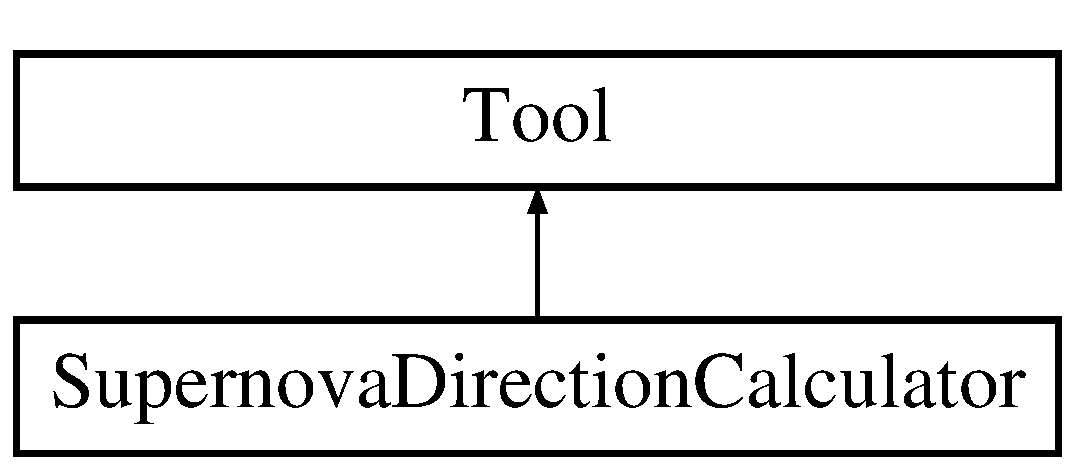
\includegraphics[height=2.000000cm]{classSupernovaDirectionCalculator}
\end{center}
\end{figure}
\subsection*{Public Member Functions}
\begin{DoxyCompactItemize}
\item 
\hypertarget{classSupernovaDirectionCalculator_aed7b11a1833767006bffac07ad3cced7}{bool {\bfseries Initialise} (std\-::string configfile, \hyperlink{classDataModel}{Data\-Model} \&data)}\label{classSupernovaDirectionCalculator_aed7b11a1833767006bffac07ad3cced7}

\item 
\hypertarget{classSupernovaDirectionCalculator_a4762604ba2382d21f239d6e71a97a174}{bool {\bfseries Execute} ()}\label{classSupernovaDirectionCalculator_a4762604ba2382d21f239d6e71a97a174}

\item 
\hypertarget{classSupernovaDirectionCalculator_a467b25370dad440342bf49be3eabd73b}{bool {\bfseries Finalise} ()}\label{classSupernovaDirectionCalculator_a467b25370dad440342bf49be3eabd73b}

\item 
\hypertarget{classSupernovaDirectionCalculator_a70ead4a641b1837728469307676330ba}{double \hyperlink{classSupernovaDirectionCalculator_a70ead4a641b1837728469307676330ba}{Get\-Event\-Weight} (double log10\-\_\-energy)}\label{classSupernovaDirectionCalculator_a70ead4a641b1837728469307676330ba}

\begin{DoxyCompactList}\small\item\em Return the weight for the event. \end{DoxyCompactList}\item 
void \hyperlink{classSupernovaDirectionCalculator_a20f7efcc68e303a9d049395663c08a03}{Calculate\-Direction} (float direction\mbox{[}3\mbox{]}, float costheta\-\_\-cut)
\end{DoxyCompactItemize}


\subsection{Member Function Documentation}
\hypertarget{classSupernovaDirectionCalculator_a20f7efcc68e303a9d049395663c08a03}{\index{Supernova\-Direction\-Calculator@{Supernova\-Direction\-Calculator}!Calculate\-Direction@{Calculate\-Direction}}
\index{Calculate\-Direction@{Calculate\-Direction}!SupernovaDirectionCalculator@{Supernova\-Direction\-Calculator}}
\subsubsection[{Calculate\-Direction}]{\setlength{\rightskip}{0pt plus 5cm}void Supernova\-Direction\-Calculator\-::\-Calculate\-Direction (
\begin{DoxyParamCaption}
\item[{float}]{direction\mbox{[}3\mbox{]}, }
\item[{float}]{costheta\-\_\-cut}
\end{DoxyParamCaption}
)}}\label{classSupernovaDirectionCalculator_a20f7efcc68e303a9d049395663c08a03}
Calculate the average S\-N neutrino direction.

Assumes events with cos(theta) $<$ costheta\-\_\-cut have no direction information. 

The documentation for this class was generated from the following files\-:\begin{DoxyCompactItemize}
\item 
User\-Tools/\-Supernova\-Direction\-Calculator/Supernova\-Direction\-Calculator.\-h\item 
User\-Tools/\-Supernova\-Direction\-Calculator/Supernova\-Direction\-Calculator.\-cpp\end{DoxyCompactItemize}

\hypertarget{classtest__vertices}{\section{test\-\_\-vertices Class Reference}
\label{classtest__vertices}\index{test\-\_\-vertices@{test\-\_\-vertices}}
}
Inheritance diagram for test\-\_\-vertices\-:\begin{figure}[H]
\begin{center}
\leavevmode
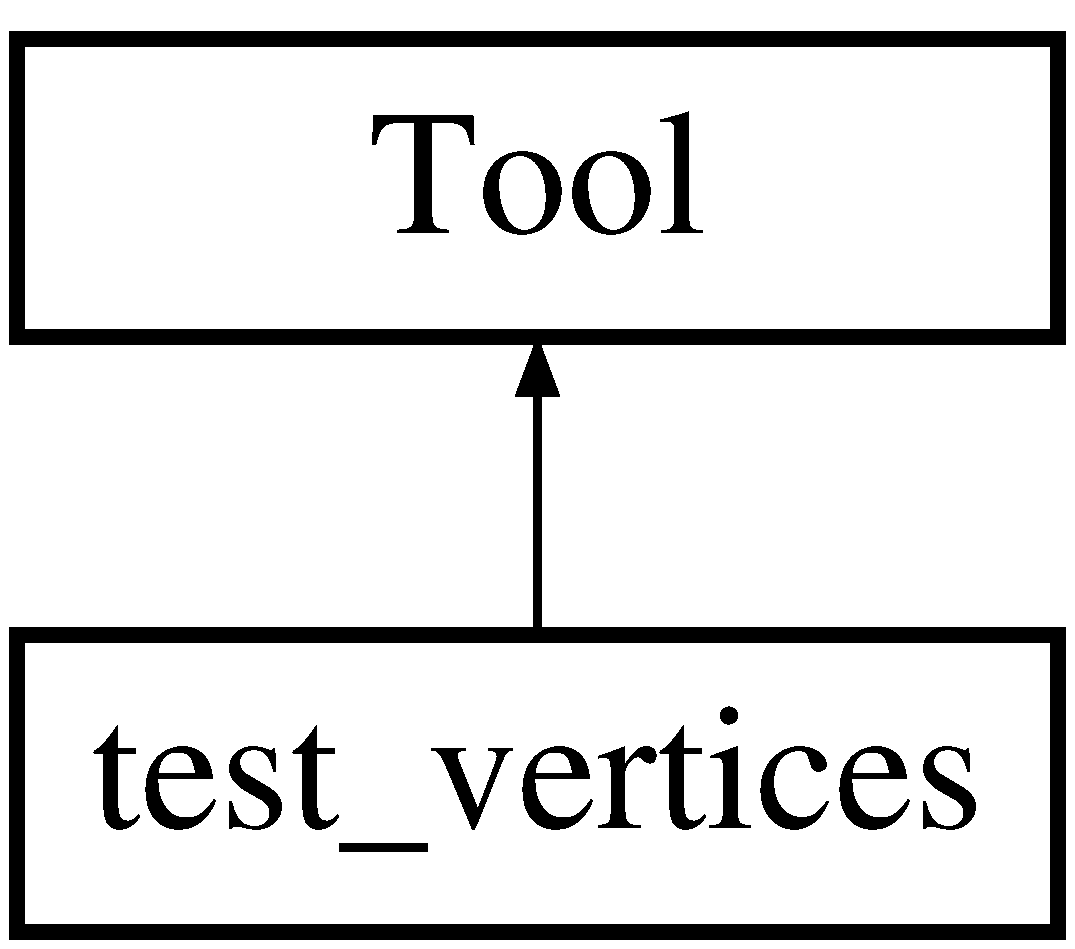
\includegraphics[height=2.000000cm]{classtest__vertices}
\end{center}
\end{figure}
\subsection*{Public Member Functions}
\begin{DoxyCompactItemize}
\item 
\hypertarget{classtest__vertices_a2f1df4bbd24e004cc0bd842d965d790c}{bool {\bfseries Initialise} (std\-::string configfile, \hyperlink{classDataModel}{Data\-Model} \&data)}\label{classtest__vertices_a2f1df4bbd24e004cc0bd842d965d790c}

\item 
\hypertarget{classtest__vertices_ae821e1dfadb82459b0dd2e5ff18075d4}{bool {\bfseries Execute} ()}\label{classtest__vertices_ae821e1dfadb82459b0dd2e5ff18075d4}

\item 
\hypertarget{classtest__vertices_abbb346ad381838ee3dcc9c294ca34c75}{bool {\bfseries Finalise} ()}\label{classtest__vertices_abbb346ad381838ee3dcc9c294ca34c75}

\end{DoxyCompactItemize}


The documentation for this class was generated from the following files\-:\begin{DoxyCompactItemize}
\item 
User\-Tools/test\-\_\-vertices/test\-\_\-vertices.\-h\item 
User\-Tools/test\-\_\-vertices/test\-\_\-vertices.\-cpp\end{DoxyCompactItemize}

\hypertarget{structThread__args}{\section{Thread\-\_\-args Struct Reference}
\label{structThread__args}\index{Thread\-\_\-args@{Thread\-\_\-args}}
}
Inheritance diagram for Thread\-\_\-args\-:\begin{figure}[H]
\begin{center}
\leavevmode
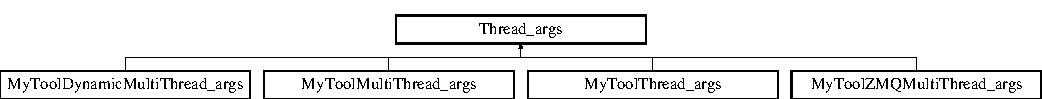
\includegraphics[height=1.333333cm]{structThread__args}
\end{center}
\end{figure}
\subsection*{Public Member Functions}
\begin{DoxyCompactItemize}
\item 
\hyperlink{structThread__args_a399b672e0f4f137fe52c141bd8c38eb1}{Thread\-\_\-args} ()
\item 
\hyperlink{structThread__args_a48650ff1135c661a730a5443ccd94f8b}{Thread\-\_\-args} (zmq\-::context\-\_\-t $\ast$contextin, std\-::string threadname, void($\ast$funcin)(std\-::string))
\item 
\hyperlink{structThread__args_af99da074784961f4953bae7e5ff67f33}{Thread\-\_\-args} (zmq\-::context\-\_\-t $\ast$contextin, std\-::string threadname, void($\ast$funcin)(\hyperlink{structThread__args}{Thread\-\_\-args} $\ast$))
\item 
virtual \hyperlink{structThread__args_ad786e0c55b4e44bc04d9ba3b813bace1}{$\sim$\-Thread\-\_\-args} ()
\end{DoxyCompactItemize}
\subsection*{Public Attributes}
\begin{DoxyCompactItemize}
\item 
\hypertarget{structThread__args_a7f2bf0637bd8774d37ddfb6096bbe448}{zmq\-::context\-\_\-t $\ast$ \hyperlink{structThread__args_a7f2bf0637bd8774d37ddfb6096bbe448}{context}}\label{structThread__args_a7f2bf0637bd8774d37ddfb6096bbe448}

\begin{DoxyCompactList}\small\item\em Z\-M\-Q context used for Z\-M\-Q socket creation. \end{DoxyCompactList}\item 
\hypertarget{structThread__args_a594f831be7ce66015a7606e023b24cf4}{std\-::string \hyperlink{structThread__args_a594f831be7ce66015a7606e023b24cf4}{Thread\-Name}}\label{structThread__args_a594f831be7ce66015a7606e023b24cf4}

\begin{DoxyCompactList}\small\item\em name of thread (deffined at creation) \end{DoxyCompactList}\item 
\hypertarget{structThread__args_a2cf8fd4407da28da635b68f47be5f8f5}{void($\ast$ \hyperlink{structThread__args_a2cf8fd4407da28da635b68f47be5f8f5}{func\-\_\-with\-\_\-string} )(std\-::string)}\label{structThread__args_a2cf8fd4407da28da635b68f47be5f8f5}

\begin{DoxyCompactList}\small\item\em function pointer to string thread \end{DoxyCompactList}\item 
\hypertarget{structThread__args_a674c5df8bb54ea3f96befbef2dfb1a78}{void($\ast$ \hyperlink{structThread__args_a674c5df8bb54ea3f96befbef2dfb1a78}{func} )(\hyperlink{structThread__args}{Thread\-\_\-args} $\ast$)}\label{structThread__args_a674c5df8bb54ea3f96befbef2dfb1a78}

\begin{DoxyCompactList}\small\item\em function pointer to thread with args \end{DoxyCompactList}\item 
\hypertarget{structThread__args_a4f71beb11e75d05269fc63ca7c19a8a9}{pthread\-\_\-t \hyperlink{structThread__args_a4f71beb11e75d05269fc63ca7c19a8a9}{thread}}\label{structThread__args_a4f71beb11e75d05269fc63ca7c19a8a9}

\begin{DoxyCompactList}\small\item\em Simple constructor underlying thread that interface is built ontop of. \end{DoxyCompactList}\item 
\hypertarget{structThread__args_a54c977a687fb1a2a82b9e9e42a5ec0f7}{zmq\-::socket\-\_\-t $\ast$ \hyperlink{structThread__args_a54c977a687fb1a2a82b9e9e42a5ec0f7}{sock}}\label{structThread__args_a54c977a687fb1a2a82b9e9e42a5ec0f7}

\begin{DoxyCompactList}\small\item\em Z\-M\-Q socket pointer is assigned in string thread,but can be sued otherwise. \end{DoxyCompactList}\item 
\hypertarget{structThread__args_a9cb8f6b709c5687bf28531bf4d808c75}{bool \hyperlink{structThread__args_a9cb8f6b709c5687bf28531bf4d808c75}{running}}\label{structThread__args_a9cb8f6b709c5687bf28531bf4d808c75}

\begin{DoxyCompactList}\small\item\em Bool flag to tell the thread to run (if not set thread goes into wait cycle. \end{DoxyCompactList}\item 
\hypertarget{structThread__args_a298b8c85c8598ecc557e2090d90a73c3}{bool \hyperlink{structThread__args_a298b8c85c8598ecc557e2090d90a73c3}{kill}}\label{structThread__args_a298b8c85c8598ecc557e2090d90a73c3}

\begin{DoxyCompactList}\small\item\em Bool flay used to kill the thread. \end{DoxyCompactList}\end{DoxyCompactItemize}


\subsection{Constructor \& Destructor Documentation}
\hypertarget{structThread__args_a399b672e0f4f137fe52c141bd8c38eb1}{\index{Thread\-\_\-args@{Thread\-\_\-args}!Thread\-\_\-args@{Thread\-\_\-args}}
\index{Thread\-\_\-args@{Thread\-\_\-args}!Thread_args@{Thread\-\_\-args}}
\subsubsection[{Thread\-\_\-args}]{\setlength{\rightskip}{0pt plus 5cm}Thread\-\_\-args\-::\-Thread\-\_\-args (
\begin{DoxyParamCaption}
{}
\end{DoxyParamCaption}
)\hspace{0.3cm}{\ttfamily [inline]}}}\label{structThread__args_a399b672e0f4f137fe52c141bd8c38eb1}
$<$ Simple constructor \hypertarget{structThread__args_a48650ff1135c661a730a5443ccd94f8b}{\index{Thread\-\_\-args@{Thread\-\_\-args}!Thread\-\_\-args@{Thread\-\_\-args}}
\index{Thread\-\_\-args@{Thread\-\_\-args}!Thread_args@{Thread\-\_\-args}}
\subsubsection[{Thread\-\_\-args}]{\setlength{\rightskip}{0pt plus 5cm}Thread\-\_\-args\-::\-Thread\-\_\-args (
\begin{DoxyParamCaption}
\item[{zmq\-::context\-\_\-t $\ast$}]{contextin, }
\item[{std\-::string}]{threadname, }
\item[{void($\ast$)(std\-::string)}]{funcin}
\end{DoxyParamCaption}
)\hspace{0.3cm}{\ttfamily [inline]}}}\label{structThread__args_a48650ff1135c661a730a5443ccd94f8b}
$<$ Construtor for thread with string \hypertarget{structThread__args_af99da074784961f4953bae7e5ff67f33}{\index{Thread\-\_\-args@{Thread\-\_\-args}!Thread\-\_\-args@{Thread\-\_\-args}}
\index{Thread\-\_\-args@{Thread\-\_\-args}!Thread_args@{Thread\-\_\-args}}
\subsubsection[{Thread\-\_\-args}]{\setlength{\rightskip}{0pt plus 5cm}Thread\-\_\-args\-::\-Thread\-\_\-args (
\begin{DoxyParamCaption}
\item[{zmq\-::context\-\_\-t $\ast$}]{contextin, }
\item[{std\-::string}]{threadname, }
\item[{void($\ast$)({\bf Thread\-\_\-args} $\ast$)}]{funcin}
\end{DoxyParamCaption}
)\hspace{0.3cm}{\ttfamily [inline]}}}\label{structThread__args_af99da074784961f4953bae7e5ff67f33}
$<$ Constrcutor for thread with args \hypertarget{structThread__args_ad786e0c55b4e44bc04d9ba3b813bace1}{\index{Thread\-\_\-args@{Thread\-\_\-args}!$\sim$\-Thread\-\_\-args@{$\sim$\-Thread\-\_\-args}}
\index{$\sim$\-Thread\-\_\-args@{$\sim$\-Thread\-\_\-args}!Thread_args@{Thread\-\_\-args}}
\subsubsection[{$\sim$\-Thread\-\_\-args}]{\setlength{\rightskip}{0pt plus 5cm}virtual Thread\-\_\-args\-::$\sim$\-Thread\-\_\-args (
\begin{DoxyParamCaption}
{}
\end{DoxyParamCaption}
)\hspace{0.3cm}{\ttfamily [inline]}, {\ttfamily [virtual]}}}\label{structThread__args_ad786e0c55b4e44bc04d9ba3b813bace1}
$<$ virtual constructor 

The documentation for this struct was generated from the following file\-:\begin{DoxyCompactItemize}
\item 
Data\-Model/Utilities.\-h\end{DoxyCompactItemize}

\hypertarget{classTimeDelta}{\section{Time\-Delta Class Reference}
\label{classTimeDelta}\index{Time\-Delta@{Time\-Delta}}
}


{\ttfamily \#include $<$Time\-Delta.\-h$>$}

\subsection*{Public Types}
\begin{DoxyCompactItemize}
\item 
\hypertarget{classTimeDelta_afe4b7adde6a0645a8ada61f39e198c8e}{typedef float \hyperlink{classTimeDelta_afe4b7adde6a0645a8ada61f39e198c8e}{short\-\_\-time\-\_\-t}}\label{classTimeDelta_afe4b7adde6a0645a8ada61f39e198c8e}

\begin{DoxyCompactList}\small\item\em Type for relative hit times within a \hyperlink{classSubSample}{Sub\-Sample}. Unit = ns. \end{DoxyCompactList}\item 
\hypertarget{classTimeDelta_a7713378e4dff3b1ed5f407260dbca5d6}{typedef int64\-\_\-t \hyperlink{classTimeDelta_a7713378e4dff3b1ed5f407260dbca5d6}{long\-\_\-time\-\_\-t}}\label{classTimeDelta_a7713378e4dff3b1ed5f407260dbca5d6}

\begin{DoxyCompactList}\small\item\em Type for absolute timestamps of a \hyperlink{classSubSample}{Sub\-Sample}. Unit = ns. \end{DoxyCompactList}\end{DoxyCompactItemize}
\subsection*{Public Member Functions}
\begin{DoxyCompactItemize}
\item 
\hypertarget{classTimeDelta_a7ea75472b12ecb4cbbd6327a1627d334}{\hyperlink{classTimeDelta_a7ea75472b12ecb4cbbd6327a1627d334}{Time\-Delta} ()}\label{classTimeDelta_a7ea75472b12ecb4cbbd6327a1627d334}

\begin{DoxyCompactList}\small\item\em Default constructor (sets all times to 0) \end{DoxyCompactList}\item 
\hypertarget{classTimeDelta_a2efa569f8caa02d8229c81ffb8905a17}{\hyperlink{classTimeDelta_a2efa569f8caa02d8229c81ffb8905a17}{Time\-Delta} (const \hyperlink{classTimeDelta}{Time\-Delta} \&)=default}\label{classTimeDelta_a2efa569f8caa02d8229c81ffb8905a17}

\begin{DoxyCompactList}\small\item\em Copy constructor (just copies all member variables) \end{DoxyCompactList}\item 
\hypertarget{classTimeDelta_a4e1bf5f12a59a250a8a947b1fc60ef1a}{\hyperlink{classTimeDelta_a4e1bf5f12a59a250a8a947b1fc60ef1a}{Time\-Delta} (double naive\-\_\-ns)}\label{classTimeDelta_a4e1bf5f12a59a250a8a947b1fc60ef1a}

\begin{DoxyCompactList}\small\item\em Constructor from naive floating point value (in ns) \end{DoxyCompactList}\item 
\hypertarget{classTimeDelta_a5b48188f53b39792626cac33924a3e85}{void \hyperlink{classTimeDelta_a5b48188f53b39792626cac33924a3e85}{Normalize} ()}\label{classTimeDelta_a5b48188f53b39792626cac33924a3e85}

\begin{DoxyCompactList}\small\item\em Ensure that the time difference stored in m\-\_\-short\-\_\-time is small and positive. \end{DoxyCompactList}\end{DoxyCompactItemize}
\subsection*{Public Attributes}
\begin{DoxyCompactItemize}
\item 
\hypertarget{classTimeDelta_a8460bb5b9864d7e42276b972f25c3d17}{\hyperlink{classTimeDelta_afe4b7adde6a0645a8ada61f39e198c8e}{short\-\_\-time\-\_\-t} \hyperlink{classTimeDelta_a8460bb5b9864d7e42276b972f25c3d17}{m\-\_\-short\-\_\-time}}\label{classTimeDelta_a8460bb5b9864d7e42276b972f25c3d17}

\begin{DoxyCompactList}\small\item\em Member for short time deltas. \end{DoxyCompactList}\item 
\hypertarget{classTimeDelta_a310ecd14cd77043ebd915f4eba2ba974}{\hyperlink{classTimeDelta_a7713378e4dff3b1ed5f407260dbca5d6}{long\-\_\-time\-\_\-t} \hyperlink{classTimeDelta_a310ecd14cd77043ebd915f4eba2ba974}{m\-\_\-long\-\_\-time}}\label{classTimeDelta_a310ecd14cd77043ebd915f4eba2ba974}

\begin{DoxyCompactList}\small\item\em Member for long time delta. \end{DoxyCompactList}\end{DoxyCompactItemize}
\subsection*{Static Public Attributes}
\begin{DoxyCompactItemize}
\item 
\hypertarget{classTimeDelta_aaed4f6897565e9a943bc0fa22d11a7e6}{static constexpr double \hyperlink{classTimeDelta_aaed4f6897565e9a943bc0fa22d11a7e6}{s\-\_\-long\-\_\-time\-\_\-unit} = 1.}\label{classTimeDelta_aaed4f6897565e9a943bc0fa22d11a7e6}

\begin{DoxyCompactList}\small\item\em Relative unit of long time member, i.\-e. long\-\_\-unit / short\-\_\-unit, both ns so = 1. \end{DoxyCompactList}\item 
\hypertarget{classTimeDelta_a03f69da08874841bc4e2434f1a3c3bfa}{static const \hyperlink{classTimeDelta}{Time\-Delta} \hyperlink{classTimeDelta_a03f69da08874841bc4e2434f1a3c3bfa}{ps} = \hyperlink{classTimeDelta}{Time\-Delta}(0.\-001)}\label{classTimeDelta_a03f69da08874841bc4e2434f1a3c3bfa}

\begin{DoxyCompactList}\small\item\em \hyperlink{classTimeDelta}{Time\-Delta} of 1 ps. \end{DoxyCompactList}\item 
\hypertarget{classTimeDelta_a18daad365109f816af53d205daa9daf9}{static const \hyperlink{classTimeDelta}{Time\-Delta} \hyperlink{classTimeDelta_a18daad365109f816af53d205daa9daf9}{ns} = \hyperlink{classTimeDelta}{Time\-Delta}(1.\-0)}\label{classTimeDelta_a18daad365109f816af53d205daa9daf9}

\begin{DoxyCompactList}\small\item\em \hyperlink{classTimeDelta}{Time\-Delta} of 1 ns. \end{DoxyCompactList}\item 
\hypertarget{classTimeDelta_a507b83ceb342b95a0c5343f488f12b34}{static const \hyperlink{classTimeDelta}{Time\-Delta} \hyperlink{classTimeDelta_a507b83ceb342b95a0c5343f488f12b34}{us} = 1000 $\ast$ \hyperlink{classTimeDelta_a18daad365109f816af53d205daa9daf9}{Time\-Delta\-::ns}}\label{classTimeDelta_a507b83ceb342b95a0c5343f488f12b34}

\begin{DoxyCompactList}\small\item\em \hyperlink{classTimeDelta}{Time\-Delta} of 1 us. \end{DoxyCompactList}\item 
\hypertarget{classTimeDelta_a46782a352ae9ed3cffd8f8a4d50828ed}{static const \hyperlink{classTimeDelta}{Time\-Delta} \hyperlink{classTimeDelta_a46782a352ae9ed3cffd8f8a4d50828ed}{ms} = 1000 $\ast$ \hyperlink{classTimeDelta_a507b83ceb342b95a0c5343f488f12b34}{Time\-Delta\-::us}}\label{classTimeDelta_a46782a352ae9ed3cffd8f8a4d50828ed}

\begin{DoxyCompactList}\small\item\em \hyperlink{classTimeDelta}{Time\-Delta} of 1 ms. \end{DoxyCompactList}\item 
\hypertarget{classTimeDelta_af7435a6440a54b9d16135bafc1d8856c}{static const \hyperlink{classTimeDelta}{Time\-Delta} \hyperlink{classTimeDelta_af7435a6440a54b9d16135bafc1d8856c}{s} = 1000 $\ast$ \hyperlink{classTimeDelta_a46782a352ae9ed3cffd8f8a4d50828ed}{Time\-Delta\-::ms}}\label{classTimeDelta_af7435a6440a54b9d16135bafc1d8856c}

\begin{DoxyCompactList}\small\item\em \hyperlink{classTimeDelta}{Time\-Delta} of 1 s. \end{DoxyCompactList}\end{DoxyCompactItemize}


\subsection{Detailed Description}
Universal data type to store both large scale (unix timestamp) and short scale (hit times) time differences

The type and unit of the long and short scale times are optimised to allow Sub\-Samples to store many hits relative to a single timestamp efficiently.

The base unit for physics simulations (at least in W\-C\-Sim) is ns, that that is the chosen as the unit for the short time scales. A signed 64 bit integer can hold values up to 2$^\wedge$63 = 9.\-22337204 x 10$^\wedge$18, which in ns would be more than 290 years. Long enough for the long time deltas.

When creating \hyperlink{classTimeDelta}{Time\-Delta} instances, one should use the unit constants to do so\-: \begin{DoxyVerb}TimeDelta t = 0.7 * TimeDelta::ms;
\end{DoxyVerb}


To convert into a naive floating point value, use them with the division operator\-: \begin{DoxyVerb}double naive_t = t / TimeDelta::us;\end{DoxyVerb}
 

The documentation for this class was generated from the following files\-:\begin{DoxyCompactItemize}
\item 
Data\-Model/Time\-Delta.\-h\item 
Data\-Model/Time\-Delta.\-cpp\end{DoxyCompactItemize}

\hypertarget{classTimeSlice}{\section{Time\-Slice Class Reference}
\label{classTimeSlice}\index{Time\-Slice@{Time\-Slice}}
}
\subsection*{Public Attributes}
\begin{DoxyCompactItemize}
\item 
\hypertarget{classTimeSlice_a34d0d4188fa5ad2416c2899f90e2e8da}{std\-::map$<$ float, Chunk $\ast$ $>$ {\bfseries chunks}}\label{classTimeSlice_a34d0d4188fa5ad2416c2899f90e2e8da}

\end{DoxyCompactItemize}


The documentation for this class was generated from the following files\-:\begin{DoxyCompactItemize}
\item 
Data\-Model/Time\-Slice.\-h\item 
Data\-Model/Time\-Slice.\-cpp\end{DoxyCompactItemize}

\hypertarget{classTriggerInfo}{\section{Trigger\-Info Class Reference}
\label{classTriggerInfo}\index{Trigger\-Info@{Trigger\-Info}}
}
\subsection*{Public Member Functions}
\begin{DoxyCompactItemize}
\item 
\hypertarget{classTriggerInfo_a29808bd2956d4561fa6e5f77bb23ab60}{void \hyperlink{classTriggerInfo_a29808bd2956d4561fa6e5f77bb23ab60}{Add\-Trigger} (Trigger\-Type\-\_\-t type, double starttime, double endtime, double triggertime, std\-::vector$<$ float $>$ info)}\label{classTriggerInfo_a29808bd2956d4561fa6e5f77bb23ab60}

\begin{DoxyCompactList}\small\item\em Add a trigger, all times in ns. \end{DoxyCompactList}\item 
\hypertarget{classTriggerInfo_a7df314e7d8cead52a2b9cf8b2d21c383}{void \hyperlink{classTriggerInfo_a7df314e7d8cead52a2b9cf8b2d21c383}{Add\-Trigger} (Trigger\-Type\-\_\-t type, \hyperlink{classTimeDelta}{Time\-Delta} readout\-\_\-start\-\_\-time, \hyperlink{classTimeDelta}{Time\-Delta} readout\-\_\-end\-\_\-time, \hyperlink{classTimeDelta}{Time\-Delta} mask\-\_\-start\-\_\-time, \hyperlink{classTimeDelta}{Time\-Delta} mask\-\_\-end\-\_\-time, \hyperlink{classTimeDelta}{Time\-Delta} trigger\-\_\-time, std\-::vector$<$ float $>$ info)}\label{classTriggerInfo_a7df314e7d8cead52a2b9cf8b2d21c383}

\begin{DoxyCompactList}\small\item\em Add a trigger. \end{DoxyCompactList}\item 
\hypertarget{classTriggerInfo_ad86bd4bc2abff60889b1b3e18a01002c}{void \hyperlink{classTriggerInfo_ad86bd4bc2abff60889b1b3e18a01002c}{Add\-Triggers} (\hyperlink{classTriggerInfo}{Trigger\-Info} $\ast$in)}\label{classTriggerInfo_ad86bd4bc2abff60889b1b3e18a01002c}

\begin{DoxyCompactList}\small\item\em Add all triggers from another \hyperlink{classTriggerInfo}{Trigger\-Info} object. \end{DoxyCompactList}\item 
\hypertarget{classTriggerInfo_a2e1db8250d38d31dc335828ce2f3bf18}{void \hyperlink{classTriggerInfo_a2e1db8250d38d31dc335828ce2f3bf18}{Clear} ()}\label{classTriggerInfo_a2e1db8250d38d31dc335828ce2f3bf18}

\begin{DoxyCompactList}\small\item\em Clear all triggers. \end{DoxyCompactList}\end{DoxyCompactItemize}
\subsection*{Public Attributes}
\begin{DoxyCompactItemize}
\item 
\hypertarget{classTriggerInfo_a7850546ae941ddd4d525d013190ea1d9}{unsigned int \hyperlink{classTriggerInfo_a7850546ae941ddd4d525d013190ea1d9}{m\-\_\-num\-\_\-triggers}}\label{classTriggerInfo_a7850546ae941ddd4d525d013190ea1d9}

\begin{DoxyCompactList}\small\item\em The number of triggers. \end{DoxyCompactList}\item 
\hypertarget{classTriggerInfo_af7dd95a327a61bdf1021a3d390413fee}{std\-::vector$<$ Trigger\-Type\-\_\-t $>$ \hyperlink{classTriggerInfo_af7dd95a327a61bdf1021a3d390413fee}{m\-\_\-type}}\label{classTriggerInfo_af7dd95a327a61bdf1021a3d390413fee}

\begin{DoxyCompactList}\small\item\em The type of Trigger. \end{DoxyCompactList}\item 
\hypertarget{classTriggerInfo_a2417285ae1e8bf98c79d88bfaff7b570}{std\-::vector$<$ \hyperlink{classTimeDelta}{Time\-Delta} $>$ \hyperlink{classTriggerInfo_a2417285ae1e8bf98c79d88bfaff7b570}{m\-\_\-readout\-\_\-start\-\_\-time}}\label{classTriggerInfo_a2417285ae1e8bf98c79d88bfaff7b570}

\begin{DoxyCompactList}\small\item\em The starting time of the trigger window. \end{DoxyCompactList}\item 
\hypertarget{classTriggerInfo_a1b27e4798addb4ebbb2cb7eb14722483}{std\-::vector$<$ \hyperlink{classTimeDelta}{Time\-Delta} $>$ \hyperlink{classTriggerInfo_a1b27e4798addb4ebbb2cb7eb14722483}{m\-\_\-readout\-\_\-end\-\_\-time}}\label{classTriggerInfo_a1b27e4798addb4ebbb2cb7eb14722483}

\begin{DoxyCompactList}\small\item\em The ending time of the trigger window. \end{DoxyCompactList}\item 
\hypertarget{classTriggerInfo_aa687342103b521c5ab70ad378efd8290}{std\-::vector$<$ \hyperlink{classTimeDelta}{Time\-Delta} $>$ \hyperlink{classTriggerInfo_aa687342103b521c5ab70ad378efd8290}{m\-\_\-mask\-\_\-start\-\_\-time}}\label{classTriggerInfo_aa687342103b521c5ab70ad378efd8290}

\begin{DoxyCompactList}\small\item\em The starting time of the hit mask. \end{DoxyCompactList}\item 
\hypertarget{classTriggerInfo_aea9dee3503ce18d1f7419c30e502b502}{std\-::vector$<$ \hyperlink{classTimeDelta}{Time\-Delta} $>$ \hyperlink{classTriggerInfo_aea9dee3503ce18d1f7419c30e502b502}{m\-\_\-mask\-\_\-end\-\_\-time}}\label{classTriggerInfo_aea9dee3503ce18d1f7419c30e502b502}

\begin{DoxyCompactList}\small\item\em The ending time of the hit mask. \end{DoxyCompactList}\item 
\hypertarget{classTriggerInfo_a296c17ef4291b793f2d4bb0acaa8d541}{std\-::vector$<$ \hyperlink{classTimeDelta}{Time\-Delta} $>$ \hyperlink{classTriggerInfo_a296c17ef4291b793f2d4bb0acaa8d541}{m\-\_\-trigger\-\_\-time}}\label{classTriggerInfo_a296c17ef4291b793f2d4bb0acaa8d541}

\begin{DoxyCompactList}\small\item\em The actual time of the trigger. \end{DoxyCompactList}\item 
\hypertarget{classTriggerInfo_ade80e80d18eae83c0c484e79dbf1207d}{std\-::vector$<$ std\-::vector$<$ float $>$ $>$ \hyperlink{classTriggerInfo_ade80e80d18eae83c0c484e79dbf1207d}{m\-\_\-info}}\label{classTriggerInfo_ade80e80d18eae83c0c484e79dbf1207d}

\begin{DoxyCompactList}\small\item\em Additional information, specific to the trigger. \end{DoxyCompactList}\end{DoxyCompactItemize}


The documentation for this class was generated from the following files\-:\begin{DoxyCompactItemize}
\item 
Data\-Model/Trigger\-Info.\-h\item 
Data\-Model/Trigger\-Info.\-cpp\end{DoxyCompactItemize}

\hypertarget{classTriggerOutput}{\section{Trigger\-Output Class Reference}
\label{classTriggerOutput}\index{Trigger\-Output@{Trigger\-Output}}
}
Inheritance diagram for Trigger\-Output\-:\begin{figure}[H]
\begin{center}
\leavevmode
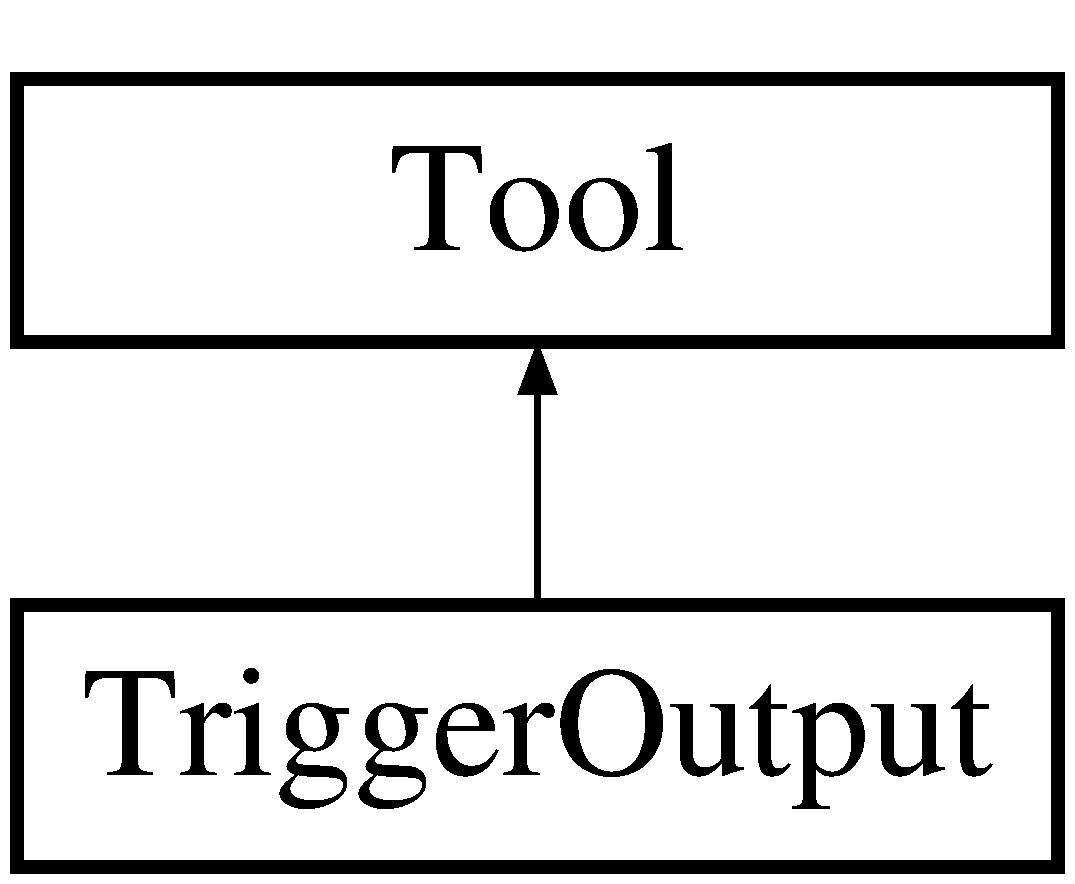
\includegraphics[height=2.000000cm]{classTriggerOutput}
\end{center}
\end{figure}
\subsection*{Public Member Functions}
\begin{DoxyCompactItemize}
\item 
\hypertarget{classTriggerOutput_a0f648ec8454242e53b16952c7639e4c6}{bool {\bfseries Initialise} (std\-::string configfile, \hyperlink{classDataModel}{Data\-Model} \&data)}\label{classTriggerOutput_a0f648ec8454242e53b16952c7639e4c6}

\item 
\hypertarget{classTriggerOutput_abb1e16e5c50df9db56d8e0e82e275b04}{bool {\bfseries Execute} ()}\label{classTriggerOutput_abb1e16e5c50df9db56d8e0e82e275b04}

\item 
\hypertarget{classTriggerOutput_a6fbc1d67082eda7453e9dbff7ba9b16e}{bool {\bfseries Finalise} ()}\label{classTriggerOutput_a6fbc1d67082eda7453e9dbff7ba9b16e}

\end{DoxyCompactItemize}


The documentation for this class was generated from the following files\-:\begin{DoxyCompactItemize}
\item 
User\-Tools/\-Trigger\-Output/Trigger\-Output.\-h\item 
User\-Tools/\-Trigger\-Output/Trigger\-Output.\-cpp\end{DoxyCompactItemize}

\hypertarget{classUtilities}{\section{Utilities Class Reference}
\label{classUtilities}\index{Utilities@{Utilities}}
}


{\ttfamily \#include $<$Utilities.\-h$>$}

\subsection*{Public Member Functions}
\begin{DoxyCompactItemize}
\item 
\hypertarget{classUtilities_a33c76f03fb859da0f0b65b80e631f0ec}{\hyperlink{classUtilities_a33c76f03fb859da0f0b65b80e631f0ec}{Utilities} (zmq\-::context\-\_\-t $\ast$zmqcontext)}\label{classUtilities_a33c76f03fb859da0f0b65b80e631f0ec}

\begin{DoxyCompactList}\small\item\em Simple constructor. \end{DoxyCompactList}\item 
\hypertarget{classUtilities_ab145803bd7737c99387c14658a292be2}{bool \hyperlink{classUtilities_ab145803bd7737c99387c14658a292be2}{Add\-Service} (std\-::string Service\-Name, unsigned int port, bool Status\-Query=false)}\label{classUtilities_ab145803bd7737c99387c14658a292be2}

\begin{DoxyCompactList}\small\item\em Broadcasts an available service (only in remote mode) \end{DoxyCompactList}\item 
\hypertarget{classUtilities_aacca3879a00425cf9aa93b0160d25b9f}{bool \hyperlink{classUtilities_aacca3879a00425cf9aa93b0160d25b9f}{Remove\-Service} (std\-::string Service\-Name)}\label{classUtilities_aacca3879a00425cf9aa93b0160d25b9f}

\begin{DoxyCompactList}\small\item\em Removes service broadcasts for a service. \end{DoxyCompactList}\item 
\hypertarget{classUtilities_acbad29ad93ad54b6feb6c9a4427ebafc}{int \hyperlink{classUtilities_acbad29ad93ad54b6feb6c9a4427ebafc}{Update\-Connections} (std\-::string Service\-Name, zmq\-::socket\-\_\-t $\ast$sock, std\-::map$<$ std\-::string, Store $\ast$ $>$ \&connections)}\label{classUtilities_acbad29ad93ad54b6feb6c9a4427ebafc}

\begin{DoxyCompactList}\small\item\em Dynamically connects a socket tp services broadcast with a specific name. \end{DoxyCompactList}\item 
\hypertarget{classUtilities_a09033997a8c4c99ebc588b3c09d45ae6}{\hyperlink{structThread__args}{Thread\-\_\-args} $\ast$ {\bfseries Create\-Thread} (std\-::string Thread\-Name, void($\ast$func)(std\-::string))}\label{classUtilities_a09033997a8c4c99ebc588b3c09d45ae6}

\item 
\hypertarget{classUtilities_ae52d1dd16b34518b2ef4de01660cb8b2}{\hyperlink{structThread__args}{Thread\-\_\-args} $\ast$ \hyperlink{classUtilities_ae52d1dd16b34518b2ef4de01660cb8b2}{Create\-Thread} (std\-::string Thread\-Name, void($\ast$func)(\hyperlink{structThread__args}{Thread\-\_\-args} $\ast$), \hyperlink{structThread__args}{Thread\-\_\-args} $\ast$args)}\label{classUtilities_ae52d1dd16b34518b2ef4de01660cb8b2}

\begin{DoxyCompactList}\small\item\em Create a thread with more complicated data exchange definned by arguments. \end{DoxyCompactList}\item 
\hypertarget{classUtilities_a3e2f8b04a35871f014628761c5e7e121}{bool \hyperlink{classUtilities_a3e2f8b04a35871f014628761c5e7e121}{Message\-Thread} (\hyperlink{structThread__args}{Thread\-\_\-args} $\ast$args, std\-::string Message, bool block=true)}\label{classUtilities_a3e2f8b04a35871f014628761c5e7e121}

\begin{DoxyCompactList}\small\item\em Send simple string to String thread. \end{DoxyCompactList}\item 
\hypertarget{classUtilities_a9aee7ba7f0e34b73b363133c8af74f92}{bool \hyperlink{classUtilities_a9aee7ba7f0e34b73b363133c8af74f92}{Message\-Thread} (std\-::string Thread\-Name, std\-::string Message, bool block=true)}\label{classUtilities_a9aee7ba7f0e34b73b363133c8af74f92}

\begin{DoxyCompactList}\small\item\em Send simple string to String thread. \end{DoxyCompactList}\item 
\hypertarget{classUtilities_a6f1c1d53b9ce59bb26c56a3bebdbb255}{bool \hyperlink{classUtilities_a6f1c1d53b9ce59bb26c56a3bebdbb255}{Kill\-Thread} (\hyperlink{structThread__args}{Thread\-\_\-args} $\ast$\&args)}\label{classUtilities_a6f1c1d53b9ce59bb26c56a3bebdbb255}

\begin{DoxyCompactList}\small\item\em Kill a thread assosiated to args. \end{DoxyCompactList}\item 
\hypertarget{classUtilities_a8c17a46ce33b0b647797f24bc859bd7a}{bool \hyperlink{classUtilities_a8c17a46ce33b0b647797f24bc859bd7a}{Kill\-Thread} (std\-::string Thread\-Name)}\label{classUtilities_a8c17a46ce33b0b647797f24bc859bd7a}

\begin{DoxyCompactList}\small\item\em Kill a thread by name. \end{DoxyCompactList}\item 
\hypertarget{classUtilities_af4091a68d8a27a3b806d029cc9b2135e}{{\footnotesize template$<$typename T $>$ }\\bool \hyperlink{classUtilities_af4091a68d8a27a3b806d029cc9b2135e}{Kill\-Thread} (T $\ast$pointer)}\label{classUtilities_af4091a68d8a27a3b806d029cc9b2135e}

\begin{DoxyCompactList}\small\item\em Kill a thread with args that inheirt form base \hyperlink{structThread__args}{Thread\-\_\-args}. \end{DoxyCompactList}\item 
\hypertarget{classUtilities_aacc51726adc504475acc998002e85136}{{\footnotesize template$<$typename T $>$ }\\bool \hyperlink{classUtilities_aacc51726adc504475acc998002e85136}{Send\-Pointer} (zmq\-::socket\-\_\-t $\ast$sock, T $\ast$pointer)}\label{classUtilities_aacc51726adc504475acc998002e85136}

\begin{DoxyCompactList}\small\item\em Send a pointer over a Z\-M\-Q socket. \end{DoxyCompactList}\item 
\hypertarget{classUtilities_ad1c8ab61a339e46afca99d5951aae713}{{\footnotesize template$<$typename T $>$ }\\bool \hyperlink{classUtilities_ad1c8ab61a339e46afca99d5951aae713}{Receive\-Pointer} (zmq\-::socket\-\_\-t $\ast$sock, T $\ast$\&pointer)}\label{classUtilities_ad1c8ab61a339e46afca99d5951aae713}

\begin{DoxyCompactList}\small\item\em Receive a pointer over a Z\-M\-Q socket. \end{DoxyCompactList}\end{DoxyCompactItemize}


\subsection{Detailed Description}
This class can be instansiated in a Tool and provides some helpful threading, dynamic socket descovery and promotion functionality

\begin{DoxyParagraph}{Author\-:}
B.\-Richards 
\end{DoxyParagraph}
\begin{DoxyParagraph}{Date\-:}
2019/05/26 18\-:34\-:00 
\end{DoxyParagraph}
Contact\-: \href{mailto:b.richards@qmul.ac.uk}{\tt b.\-richards@qmul.\-ac.\-uk} 

The documentation for this class was generated from the following files\-:\begin{DoxyCompactItemize}
\item 
Data\-Model/Utilities.\-h\item 
Data\-Model/Utilities.\-cpp\end{DoxyCompactItemize}

\hypertarget{classWCSimASCIReader}{\section{W\-C\-Sim\-A\-S\-C\-I\-Reader Class Reference}
\label{classWCSimASCIReader}\index{W\-C\-Sim\-A\-S\-C\-I\-Reader@{W\-C\-Sim\-A\-S\-C\-I\-Reader}}
}
Inheritance diagram for W\-C\-Sim\-A\-S\-C\-I\-Reader\-:\begin{figure}[H]
\begin{center}
\leavevmode
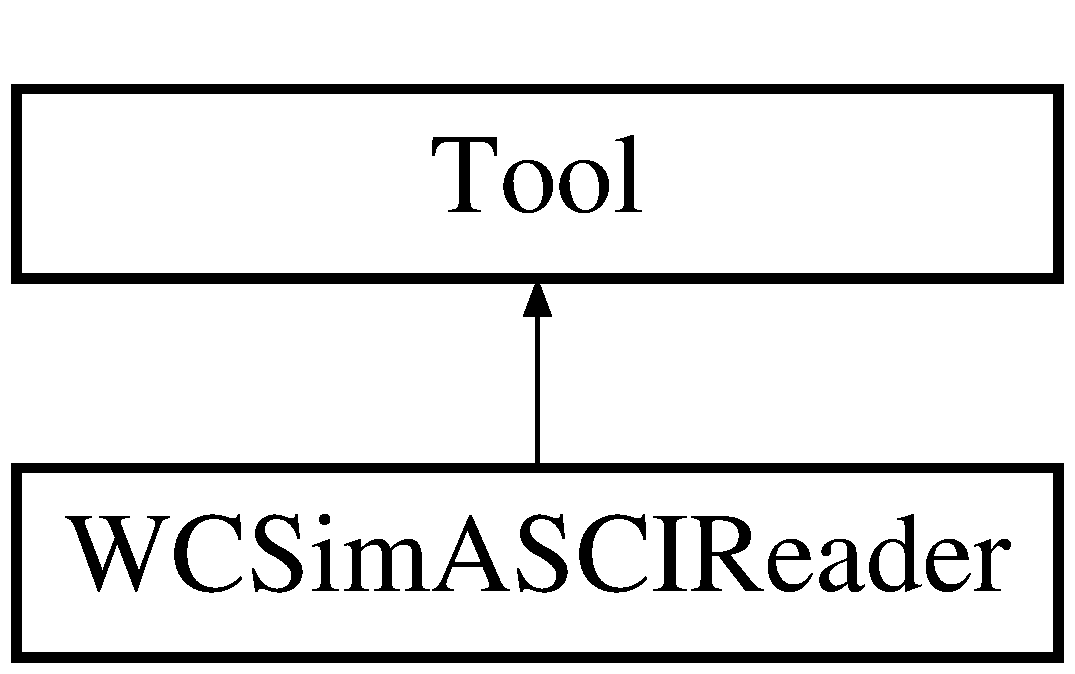
\includegraphics[height=2.000000cm]{classWCSimASCIReader}
\end{center}
\end{figure}
\subsection*{Public Member Functions}
\begin{DoxyCompactItemize}
\item 
\hypertarget{classWCSimASCIReader_a306f7247090985ac8347817dc3c8b316}{bool {\bfseries Initialise} (std\-::string configfile, \hyperlink{classDataModel}{Data\-Model} \&data)}\label{classWCSimASCIReader_a306f7247090985ac8347817dc3c8b316}

\item 
\hypertarget{classWCSimASCIReader_a149c2fc15239bb4e450456e41958cb72}{bool {\bfseries Execute} ()}\label{classWCSimASCIReader_a149c2fc15239bb4e450456e41958cb72}

\item 
\hypertarget{classWCSimASCIReader_a41815a094817b22741cd2dd984cdd52e}{bool {\bfseries Finalise} ()}\label{classWCSimASCIReader_a41815a094817b22741cd2dd984cdd52e}

\end{DoxyCompactItemize}


The documentation for this class was generated from the following files\-:\begin{DoxyCompactItemize}
\item 
User\-Tools/\-W\-C\-Sim\-A\-S\-C\-I\-Reader/W\-C\-Sim\-A\-S\-C\-I\-Reader.\-h\item 
User\-Tools/\-W\-C\-Sim\-A\-S\-C\-I\-Reader/W\-C\-Sim\-A\-S\-C\-I\-Reader.\-cpp\end{DoxyCompactItemize}

\hypertarget{classWCSimReader}{\section{W\-C\-Sim\-Reader Class Reference}
\label{classWCSimReader}\index{W\-C\-Sim\-Reader@{W\-C\-Sim\-Reader}}
}
Inheritance diagram for W\-C\-Sim\-Reader\-:\begin{figure}[H]
\begin{center}
\leavevmode
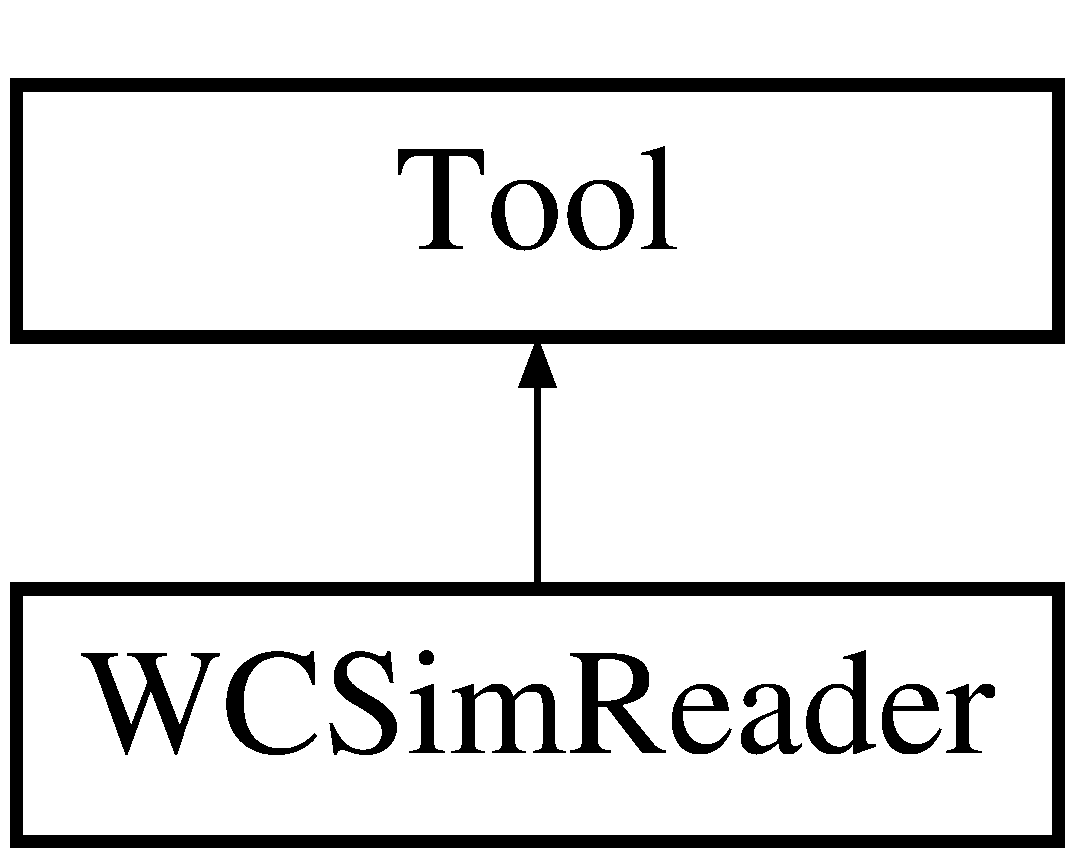
\includegraphics[height=2.000000cm]{classWCSimReader}
\end{center}
\end{figure}
\subsection*{Public Member Functions}
\begin{DoxyCompactItemize}
\item 
\hypertarget{classWCSimReader_a6b68e5354bd307f85345b776977943c9}{bool {\bfseries Initialise} (std\-::string configfile, \hyperlink{classDataModel}{Data\-Model} \&data)}\label{classWCSimReader_a6b68e5354bd307f85345b776977943c9}

\item 
\hypertarget{classWCSimReader_a846289c0eb870110a4961257832203c5}{bool {\bfseries Execute} ()}\label{classWCSimReader_a846289c0eb870110a4961257832203c5}

\item 
\hypertarget{classWCSimReader_a806d70ee9a5522b85feea663d34799ff}{bool {\bfseries Finalise} ()}\label{classWCSimReader_a806d70ee9a5522b85feea663d34799ff}

\end{DoxyCompactItemize}


The documentation for this class was generated from the following files\-:\begin{DoxyCompactItemize}
\item 
User\-Tools/\-W\-C\-Sim\-Reader/W\-C\-Sim\-Reader.\-h\item 
User\-Tools/\-W\-C\-Sim\-Reader/W\-C\-Sim\-Reader.\-cpp\end{DoxyCompactItemize}

\hypertarget{structutil_1_1Window}{\section{util\-:\-:Window Struct Reference}
\label{structutil_1_1Window}\index{util\-::\-Window@{util\-::\-Window}}
}


Contains the start and end of a time window, along with an I\-D (nominally trigger number)  




{\ttfamily \#include $<$Utilities.\-h$>$}

\subsection*{Public Member Functions}
\begin{DoxyCompactItemize}
\item 
\hypertarget{structutil_1_1Window_a8d07478c6ec86580a85651ff8aee7bbd}{{\bfseries Window} (int trigger\-\_\-num, \hyperlink{classTimeDelta}{Time\-Delta} start, \hyperlink{classTimeDelta}{Time\-Delta} end)}\label{structutil_1_1Window_a8d07478c6ec86580a85651ff8aee7bbd}

\end{DoxyCompactItemize}
\subsection*{Public Attributes}
\begin{DoxyCompactItemize}
\item 
\hypertarget{structutil_1_1Window_a0e08b9541333436563d90bedb5a05395}{int {\bfseries m\-\_\-trigger\-\_\-num}}\label{structutil_1_1Window_a0e08b9541333436563d90bedb5a05395}

\item 
\hypertarget{structutil_1_1Window_aa200771caef3a1a6bd46481a67739ca3}{\hyperlink{classTimeDelta}{Time\-Delta} {\bfseries m\-\_\-start}}\label{structutil_1_1Window_aa200771caef3a1a6bd46481a67739ca3}

\item 
\hypertarget{structutil_1_1Window_a396a04d14679767e54358145d933fc85}{\hyperlink{classTimeDelta}{Time\-Delta} {\bfseries m\-\_\-end}}\label{structutil_1_1Window_a396a04d14679767e54358145d933fc85}

\end{DoxyCompactItemize}


\subsection{Detailed Description}
Contains the start and end of a time window, along with an I\-D (nominally trigger number) 

The documentation for this struct was generated from the following file\-:\begin{DoxyCompactItemize}
\item 
Data\-Model/Utilities.\-h\end{DoxyCompactItemize}

\hypertarget{structZMQMyToolMultiThread__args}{\section{Z\-M\-Q\-My\-Tool\-Multi\-Thread\-\_\-args Struct Reference}
\label{structZMQMyToolMultiThread__args}\index{Z\-M\-Q\-My\-Tool\-Multi\-Thread\-\_\-args@{Z\-M\-Q\-My\-Tool\-Multi\-Thread\-\_\-args}}
}


{\ttfamily \#include $<$My\-Tool\-Z\-M\-Q\-Multi\-Thread.\-h$>$}



\subsection{Detailed Description}
This is a struct to place data you want your thread to acess or exchange with it. The idea is the datainside is only used by the threa\textbackslash{} d and so will be thread safe

\begin{DoxyParagraph}{Author\-:}
B.\-Richards 
\end{DoxyParagraph}
\begin{DoxyParagraph}{Date\-:}
2019/05/28 10\-:44\-:00 
\end{DoxyParagraph}
Contact\-: \href{mailto:b.richards@qmul.ac.uk}{\tt b.\-richards@qmul.\-ac.\-uk} 

The documentation for this struct was generated from the following file\-:\begin{DoxyCompactItemize}
\item 
User\-Tools/template/My\-Tool\-Z\-M\-Q\-Multi\-Thread.\-h\end{DoxyCompactItemize}

%--- End generated contents ---

% Index
\newpage
\phantomsection
\addcontentsline{toc}{part}{Index}
\printindex

\end{document}
